\documentclass[11pt]{aghdpl}
% \documentclass[en,11pt]{aghdpl}  % praca w języku angielskim

% Lista wszystkich języków stanowiących języki pozycji bibliograficznych użytych w pracy.
% (Zgodnie z zasadami tworzenia bibliografii każda pozycja powinna zostać utworzona zgodnie z zasadami języka, w którym dana publikacja została napisana.)
\usepackage[english,polish]{babel}

% Użyj polskiego łamania wyrazów (zamiast domyślnego angielskiego).
\usepackage{polski}

\usepackage[utf8]{inputenc}

% dodatkowe pakiety

\usepackage{mathtools}
\usepackage{amsfonts}
\usepackage{amsmath}
\usepackage{amsthm}
\usepackage{float}

% --- < bibliografia > ---

\usepackage[
style=numeric,
sorting=none,
%
% Zastosuj styl wpisu bibliograficznego właściwy językowi publikacji.
language=autobib,
autolang=other,
% Zapisuj datę dostępu do strony WWW w formacie RRRR-MM-DD.
urldate=iso8601,
% Nie dodawaj numerów stron, na których występuje cytowanie.
backref=false,
% Podawaj ISBN.
isbn=true,
% Nie podawaj URL-i, o ile nie jest to konieczne.
url=false,
%
% Ustawienia związane z polskimi normami dla bibliografii.
maxbibnames=3,
% Jeżeli używamy BibTeXa:
backend=bibtex
]{biblatex}

\usepackage{csquotes}
% Ponieważ `csquotes` nie posiada polskiego stylu, można skorzystać z mocno zbliżonego stylu chorwackiego.
\DeclareQuoteAlias{croatian}{polish}

\addbibresource{bibliografia.bib}

% Nie wyświetlaj wybranych pól.
%\AtEveryBibitem{\clearfield{note}}


% ------------------------
% --- < listingi > ---

% Użyj czcionki kroju Courier.
\usepackage{courier}

\usepackage{listings}
\lstloadlanguages{TeX}

\lstset{
	literate={ą}{{\k{a}}}1
	{ć}{{\'c}}1
	{ę}{{\k{e}}}1
	{ó}{{\'o}}1
	{ń}{{\'n}}1
	{ł}{{\l{}}}1
	{ś}{{\'s}}1
	{ź}{{\'z}}1
	{ż}{{\.z}}1
	{Ą}{{\k{A}}}1
	{Ć}{{\'C}}1
	{Ę}{{\k{E}}}1
	{Ó}{{\'O}}1
	{Ń}{{\'N}}1
	{Ł}{{\L{}}}1
	{Ś}{{\'S}}1
	{Ź}{{\'Z}}1
	{Ż}{{\.Z}}1,
	basicstyle=\footnotesize\ttfamily,
}

% ------------------------

\AtBeginDocument{
	\renewcommand{\tablename}{Tabela}
	\renewcommand{\figurename}{Rys.}
}

% ------------------------
% --- < tabele > ---

\usepackage{array}
\usepackage{tabularx}
\usepackage{multirow}
\usepackage{booktabs}
\usepackage{makecell}
\usepackage[flushleft]{threeparttable}

% defines the X column to use m (\parbox[c]) instead of p (`parbox[t]`)
\newcolumntype{C}[1]{>{\hsize=#1\hsize\centering\arraybackslash}X}


%---------------------------------------------------------------------------

\author{Filip Biernat}
\shortauthor{F. Biernat}

\titlePL{Metody mediacji wiedzy w systemach affective computing}
\titleEN{Methods for knowledge mediation in affective computing systems}


\shorttitlePL{Metody mediacji wiedzy w systemach affective computing}
\shorttitleEN{Methods for knowledge mediation in affective computing systems}

\thesistype{Praca dyplomowa magisterska}

\supervisor{dr inż. Szymon Bobek}

\degreeprogramme{Informatyka}

\date{2019}

\department{Katedra Informatyki Stosowanej}

\faculty{Wydział Elektrotechniki, Automatyki,\protect\\[-1mm] Informatyki i Inżynierii Biomedycznej}

\acknowledgements{}

\setlength{\cftsecnumwidth}{10mm}

%---------------------------------------------------------------------------
\setcounter{secnumdepth}{4}
\brokenpenalty=10000\relax

\begin{document}
	
	\titlepages
	
	% Ponowne zdefiniowanie stylu `plain`, aby usunąć numer strony z pierwszej strony spisu treści i poszczególnych rozdziałów.
	\fancypagestyle{plain}
	{
		% Usuń nagłówek i stopkę
		\fancyhf{}
		% Usuń linie.
		\renewcommand{\headrulewidth}{0pt}
		\renewcommand{\footrulewidth}{0pt}
	}
	
	\setcounter{tocdepth}{2}
	\tableofcontents
	\clearpage
	
	\chapter{Wprowadzenie}
\label{cha:wprowadzenie}

%---------------------------------------------------------------------------

\section{Cel pracy}
\label{sec:celPracy}

Celem pracy jest zaprojektowanie, implementacja i ewaluacja mechanizmu pozyskiwania wiedzy o  stanie emocjonalnym użytkownika w systemach \textit{affective computing}.

W szczególności w~ramach pracy przeprowadzona zostanie analiza istniejących rozwiązań, na bazie których opracowane zostało rozwiązanie pozwalające na odpytywanie użytkownika o stan emocjonalny w sposób możliwie nieintruzywny.  Na potrzeby pracy zaprojektowana i zaimplementowana zostanie aplikacja mobilna pozwalająca na uczynienie jawnej mediacji wiedzy możliwie nieintruzywną (poprzez wnioskowanie oparte na monitorowaniu czynników zewnętrznych) oraz na przeprowadzenie niejawnej mediacji (z wykorzystaniem aparatu fotograficznego telefonu) wykorzystując znajomość tzw. kontekstu czyli informacji o otoczeniu użytkownika i dysponując możliwością dynamicznego reagowania na zmiany kontekstu w czasie rzeczywistym.. 

Rozwiązanie zostanie poddane ewaluacji przeprowadzając badanie wśród grona użytkowników, którzy następnie zostaną przepytani, a wyniki kwestionariuszy zostaną opisane w niniejszej pracy.


%---------------------------------------------------------------------------

\section{Zastosowania wykrywania emocji}
\label{sec:zastosowaniaWykrywaniaEmocji}

Nasz świat powoli staje się światem, w którym maszyna potrafi rozpoznawać emocje. Wraz z rozwojem technologii pojawiają się i będą pojawiać kolejne systemy zdolne do wykrywania emocji użytkownika i wykorzystywania ich, aby lepiej spełniać swoje zadania:

\begin{itemize}	
	\item Już teraz pojawiają się pierwsze gry komputerowe wykorzystujące informacje o stanie emocjonalnym użytkownika. Przykładem może być \cite{nalepa2017affective}. Dla aplikacji budujących alternatywny świat, zwłaszcza w coraz popularniejszej wirtualnej czy rozszerzonej rzeczywistości, wiedza o stanie emocjonalnym użytkownika byłaby bezcenna.
	
	\item Na rynku pojawiają się też pierwsze systemy e-learningowe wykorzystujące dodatkowe informacje afektywne do lepszego dopasowania tempa i materiału. Przykładem może być \cite{feidakis2012design}.
	
	\item Praca \cite{hung2016predicting} opisuje zastosowanie wykrywania emocji w medycynie. Takie systemy mogą znaleźć zastosowanie na przykład w walce z depresją, którą już teraz nazywa się chorobą cywilizacyjną dwudziestego pierwszego wieku.
	
	\item Pojawiają się także specjalne systemy afektywne zaprojektowane z myślą o osobach starszych. Oprogramowanie takie jak \cite{yu2014emotion} może wezwać karetkę czy inną pomoc, a także świadczyć inne udogodnienia reagując w czasie rzeczywistym na informacje o stanie emocjonalnym.
	
	\item Naturalnym przykładem zastosowania wykrywania emocji są systemy rekomendacyjne. Platformy multimedialne i streamingowe takie jak Netflix, Spotify, Twitch czy Youtube mogłyby wykorzystywać dodatkowe informacje, aby jeszcze lepiej wybierać muzykę czy filmy.
	
	\item Systemy rekomendacji mają także olbrzymie znaczenie w sprzedaży. Propozycje systemów sprzedających takich jak Amazon, Allegro czy Aliexpress dysponując w przyszłości informacjami o emocjach mogłyby być znacznie dokładniejsze.
\end{itemize}

%---------------------------------------------------------------------------

\section{Gromadzenie danych}
\label{sec:gromadzenieDanych}

Telefon komórkowy potrafi odczytać położenie za pomocą żyroskopu, czy tekst za pomocą dotykowej klawiatury. Idea \textit{HowAreYou} -- aplikacji stworzonej na potrzeby niniejsze pracy -- polega na tym, żeby te ograniczone sygnały połączyć i za ich pomocą odczytać nastrój użytkownika. Smartfon może też zrobić zdjęcie kamerą -- za pomocą fotografii już teraz można całkiem dokładnie określić nastrój użytkownika. Można też wprost zapytać użytkownika telefonu –- jeżeli nie nadużyjemy tego rozwiązania, stwarza ono szeroki wachlarz możliwości.

Jednym z najważniejszych wyzwań związanych z projektowaniem aplikacji przetwarzajacych dane użytkwonika jest kwestia prywatności. Człowiek, co naturalne, lubi strzec swojej niezależności. Zrezygnuje z wykorzystywania przygotowanego rozwiązania, jeżeli będzie nieustannie niepokojony, albo poczuje, że traci kontrolę nad danymi, które trafiają do bazy. Konieczne jest zaprojektowanie takiego systemu, który da użytkownikowi możliwość wyboru i pewność, że treści, które udostępnia, są przez niego kontrolowane i całkowicie bezpieczne.
	\chapter{Mechanizmy mediacji wiedzy}
\label{cha:mechanizmyMediacjiWiedzy}

%---------------------------------------------------------------------------

\section{Obszary zastosowań}
\label{sec:obszaryZastosowan}

Z mechanizmami mediacji wiedzy spotykamy się na co dzień -- od prostych, analogowych form zebrania tzw. \textit{feedbacku} od użytkownika do bardziej zaawansowanych systemów cyfrowych.

Wiele instytucji publicznych (jak urzędy \cite{umkrakow}, szkoły, uczelnie \cite{wgigagh}) oraz prywatnych przedsiębiorstw gromadzi informacje od petentów czy klientów na przykład w formie dobrowolnych kwestionariuszy w~~celu podniesienia jakości świadczonych usług. W marketach popularność zyskują na przykład przyciski wformie emotikon, które klient może  nacisnąć przy wyjściu, przekazując czy jest zadowolony.

\begin{figure}[H]
	\centering
	\includegraphics[scale=0.8]{rozdzial2/Biedronka.jpg}
	\caption{Przykład prostego mechanizmu mediacji wiedzy w supermarketach sieci Biedronka. Użytkownik przekazuje informację o stanie afektywnym klikając w odpowiednią emotikonę.}
\end{figure}

	
Opinia osób jest szczególnie ważna w systemach tworzonych w sposób zorientowany na użytkownika (ang. \textit{user-centered design}). Na przykład w branży projektowania stron internetowych przy projektowaniu nowoczesnych, profesjonalnych rozwiązań, w fazie początkowych testów, a czasem również w~fazie regularnego funkcjonowania udostępnia się użytkownikowi kwestionariusz w celu poprawy jakości czy nawet buduje z grona użytkowników zespoły scrumowe odpowiedzialne, za przekazanie swoich odczuć związanych z designem \cite{uxdesign}.
	
Część systemów rekomendacji zaczęła już wykorzystywać mediację wiedzy. To rozwiązanie staje się coraz popularniejsze na przykład pośród platform zawodowo-biznesowych wykorzystywanych do poszukiwania pracy \cite{careerexplorer}.
	
Omawiane tu mechanizmy znajdują zastosowanie również w medycynie. Przykładem może być wspomniana już w poprzednim rozdziale aplikacja zaprojektowana w ramach pracy \cite{hung2016predicting} stanowiąca próbę walki z depresją.


%---------------------------------------------------------------------------

\section{Jawne metody mediacji wiedzy}
\label{sec:jawneMetodyMediacjiWiedzy}

Pierwszą z~kategorii metod mediacji wiedzy są metody jawne. Oznacza to, że w~proces mediacji zaangażowany jest sam użytkownik. To rozwiązanie ma swoje wady i zalety. Z pewnością największą zaletą jest skuteczność rozwiązania -- nikt nie wie więcej o stanie emocji niż sam użytkownik. Z kolei główną wadą jest fakt, że takie badanie może okazać się uciążliwe i irytujące, a na dłuższą metę zbytnio ingerujące w~życie człowieka, czy wręcz niemożliwe.

Przykładem jawnej metody może być praca \cite{EmiliaPieczonka}. W badaniach, jakie przeprowadziła, ''grupa użytkowników korzystajaca z~telefonu Android i aplikacji mobilnej, używała podczas codziennych czynności urządzenia sensorycznego na swoim nadgarstku i odpowiadała na pytania dotyczące ich samopoczucia''.

Warto również zwrócić uwagę na pracę \cite{ArkadiuszLis}. Zostało w~niej wybrane w~oparciu o literaturę naukową kilka najbardziej obiecujących sposobów mediacji wiedzy. Następnie zaimplementowano zestaw widgetów, z~pomocą których użytkownik ''powinien być w~stanie subiektywnie określić stan emocjonalny (...), a następnie przekazać tą informację do systemu''.

W pracy opisanej w~artykule \cite{hung2016predicting} naukowcy we współpracy z~psychiatrą stworzyli system, z~którego pomocą badany z~wykorzystaniem kolorowego suwaka może określić poziom swojego niepokoju czy gniewu. Badacze skupili się przede wszystkim nie na sensorach, ale na wzorcach korzystania z~telefonu udostępniach przez system operacyjnych takich jak wykonywanie połączeń, pisanie SMSów czy lokalizacja.

Mediacja nie musi odbywać się z~wykorzystaniem ekranu. Na rynku pojawiają się rozwiązania, w~których system głosowy taki jak Alexa, Asystent Google, Cortana czy Siri podczas rozmowy sam wypytuje użytkownika o nastrój.


%---------------------------------------------------------------------------

\section{Niejawne metody mediacji wiedzy}
\label{sec:niejawneMetodyMediacjiWiedzy}

Drugą kategorią metod mediacji wiedzy są metody niejawne. De facto sprowdza się to do braku bezpośredniego uczestnictwa człowieka w~przekazywaniu wiedzy. Oczywiście człowiek jest zaangażowany w~proces na przykład poprzez wykonywanie różnych czynności, ale nie zostanie nigdy zapytany wprost. Podobnie jak pierwsza kategoria, ta druga również ma swoje wady i zalety. Do zalet można zaliczyć wygodę -- korzystanie z~tych metod jest nieinwazyjne, nie ingeruje w~codzienną egzystencję. Minusem jest oczywiście mniejsza skuteczność.

Przykładem takiej mediacji może być praca \cite{zhang2011feature}, w~której naukowcy podejmują próby rozpoznania aktywności człowieka wykorzystując czujniki multimodalne. Do przetworzenia danych wykorzystywane są algorytmy wyboru cech.

Podobną metodą wykorzystali naukowcy w~pracy \cite{dai2010mobile} wykorzystując stworzony przez siebie model matematyczny w~celu określenia czy kierowca samochodu jest trzeźwy czy pijany.


%---------------------------------------------------------------------------

\section{Pozyskiwanie wiedzy o stanie emocjonalnym w~systemach \textit{affective computing}}
\label{sec:pozyskiwanieWiedzyOStanieEmocjonalnymWSystemachAffectiveComputing}

\textit{Affective computing} jest paradygmatem zaproponowanym przez Rosalind Picard z~Laboratorium Mediów MIT w~1997 roku\cite{picard1997affective}.

Wykorzystuje on rezultaty inżynierii biomedycznej, psychologii i sztucznej inteligencji. Celem jest pozwolenie systemom komputerowym wykrywać, wykorzystywać, a nawet wyrażać emocje\cite{nalepa2017affective}.

Przykładem pozyskiwania wiedzy może być gra wideo \textit{Bridge Scroll-runner} stworzona w~ramach pracy \cite{nalepa2017affective}. Naukowcy rozszerzyli możliwości gry wykorzystując czujniki tętna, temperatury skóry oraz reakcji galwanicznej skóry.

Rosaling Picard w~swojej pionierskiej pracy \cite{picard1997affective} jako przykład podaje komputerowy system uczący gry na pianinie. Taki system mógłby być znacznie skuteczniejszy od klasycznego systemu dysponując możliwością wyczuwania zainteresowania, przyjemności i smutku.

Wraz z rozwojem technologii metody pozyskiwania wiedzy o stanie emocjonalnym stają się coraz bardziej zaawansowane. Realizacja kolejnych technik jest dla twórców swego rodzaju wyzwaniem, ale stanowi okazję do przeprowadzenia coraz dokładniejszej analizy ludzkich emocji. Poniżej przedstawiono przegląd znanych metod pozyskiwanie wiedzy o stanie emocjonalnym w~systemach \textit{affective computing}:

\begin{itemize}	
	\item Najbardziej podstawowymi metodami są techniki analogowe. Kwestionariusz może być przeprowadzony w sposób całkowicie niewspomagany cyfrowo. Sposób polega na tym, że osobie badanej zostaje przedstawiony zestaw pytań. Mamy tutaj szeroki zakres możliwości. Pytania mogą być wypełniane przez uczestnika badania lub zadawane przez ankietera -- w tym drugim przypadku ankieter może próbować również skonstruować kolejne, bardziej dokładne pytania. Kwestionariusz może być wypełniony przez osobę jednorazowo lub wypełniany w sposób regularny -- te bardziej systematyczne z reguły dają lepsze rezutaty. Same pytania mogą dotyczyć stanu obecnego, mogą też dotyczyć stanów z przeszłości. W bardziej zaawansowanych wersjach dodatkowe pytania mogą pomóc zrozumieć nie tylko stan, ale także czynniki czy okoliczności, które przyczyniły się do jego zmiany. Jedną z zalet kwestionariuszy jest fakt, że można zdobyć info bez konieczności poświęcenia czasu i zasobów na projektowanie i implementacje bardziej zaawansowanego techologicznie rozwiązania. Przeprowadzony w sposób dokładny i regularny może dać zadowalające wyniki. Trzeba też pamiętać, że przez lata była to jedyna dość skuteczna metoda. Z kolei zedycowaną wadą jest fakt, że metoda ta może być bardzo obciążająca zarówno dla osoby badanej jak i badającej. Im bardziej szczegółowe badanie, z tym większą uciążliwością się to wiąże. Samo podejście może się okazać czasochłonne, a wyniki trudne do opracowania.
	
	\item Inną, nieco bardziej zaawansowaną metodą jest wykonywanie połączeń telefonicznych tak jak w~badaniu \cite{courvoisier2010psychometric}. W porównaniu do techniki analogowej jest to bardziej wymagające przede wszystkim logistycznie, a główną wadą może być znaczne obciążenie zarówno strony badającej jak i badanej.
	
	\item Odmienne podejście prezentują automatyczne techniki gromadzenia informacji o stanie emocjonalnym użytkownika. Mowa tu o systemach, które regularnie co jakiś czas przedstawiają osobie badanej pytanie i zapisują odpowiedź. W tym przypadku wyzwaniem jest wybór platformy i przede wszystkim stworzenie sytemu, ale zmiana podejścia daje duże zyski w postaci automatyzacji całego procesu.
	
	\item Bardziej zaawansowanym sposobem jest wybór zakresów godzinowych (czyli pór dnia) poprzez eksperta domenowego i tym samym ograniczenie odpytywania uczestnika badania tylko do określonych przedziałów. Technika mediacji o losowej porze, ale tylko wewnątrz ustalonego wcześniej zakresu została zastosowana m.in. w pracy \cite{bailon2019smartphone}. W tym przypadku zaletą jest nieznaczne obciążenie techniczne w stosunku do poprzedniej metody. Zmiana w postaci zawężenia okresów odpytywania niewielkim kosztem sprawia, że system jest bardziej przyjazny dla użytkownika.
	
	\item Ostatnią z przytoczonych tutaj metod jest odpytywanie użytkownika w czasie rzeczywistym w~oparciu o wnioskowanie na podstawie danych z otoczenia. System, który jest świadomy ,,kontekstu'' (ang. \textit{context-aware system}) jest w stanie zminimalizować uciążliwość dla użytkownika odpytując na przykład tylko w momentach, kiedy nie jest pewny stanu emocjonalnego (bo na przykład może go zbadać również w sposób niejawny), albo zaobserwował znaczącą zmianę jednego z czynników otoczenia. Właśnie taka zaawansowana aplikacja stworzona zostanie w ramach niniejszej pracy.
\end{itemize}

W pracy zastosowano zarówno metody jawne jak i niejawne. W celu pozyskania wiedzy o stanie emocjonalnym zdecydowano się na syntezę odpowiedzi użytkownika i działania automatycznego systemu. Odpowiedzi użytkownika mogą być realizowane wprost poprzez aktywność z~listą emocji (jak na powyższym diagramie) i emotikon do wyboru lub (bardziej psychologicznie) z~wykorzystaniem palety kolorów. Automatyczny system wykorzystuje zewnętrzne API, które zwraca wartości wykrytych emocji na podstawie fotografii, która została wcześniej wykonana. W przyszłości możliwe jest rozszerzenie aplikacji o system uczący się rozpoznawać emocje z~sensorów AWARE porównując duże ilości danych niezrozumiałych z~sensorów z~danymi otrzymanymi z~wykorzystaniem jawnych i niejawnych metod mediacji wiedzy.

\begin{figure}[H]
	\centering
	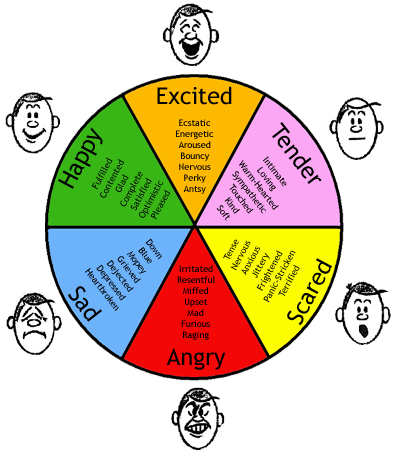
\includegraphics[scale=1]{rozdzial2/ModelEkmana.png}
	\caption{Koło podstawowych emocji (szczęście, podekscytowanie, rozczulenie, strach, gniew i smutek) i ich mimicznych ekspresji.}
\end{figure}


	\chapter{Architektura rozwiązania}
\label{cha:architekturaRozwiazania}

%---------------------------------------------------------------------------

\section{Zarys architektury}
\label{sec:zarysArchitektury}

Trzon rozwiązania stanowi plugin \textit{HowAreYou}. Plugin działa w ramach frameworka AWARE. Do wykorzystywania pluginu konieczna jest więc aplikacja kliencka \textit{AWARE}. Ponadto wewnątrz pluginu wkompilowana jest również biblioteka rdzeniowa \textit{AWARE-core}. Sam plugin działa więc jako niezależna aplikacja i jako osobna instancja \textit{AWARE}. Aplikacja kliencka służy jedynie do konfiguracji rozszerzenia.

\begin{figure}[H]
	\centering
	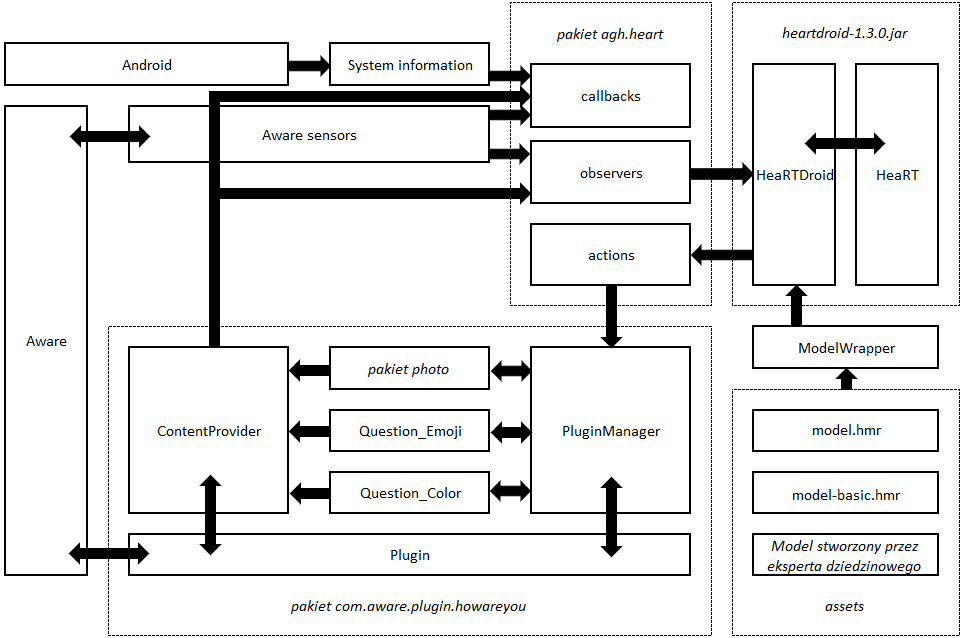
\includegraphics[scale=0.8]{rozdzial3/ArchitekturaSchemat.png}
	\caption{Schemat przedstawiający ogólną architekturę rozwiązania.}
\end{figure}

Wewnątrz pluginu wkompilowana jest również biblioteka silnika wnioskującego \textit{HeaRTDroid}. Zawarty wewnątrz pluginy pakiet \textit{agh.heart} (\textit{HeaRT-AWARE}) stanowi proxy pomiędzy zasadniczą częścią aplikacji a samym silnikiem. Plugin zawiera też kod \textit{XTT2} modeli wnioskujących dla silnika oraz implementuje rozwiązania, dzięki którym może komunikować się z użytkownikiem, gromadzić dane i przesyłać te dane do wspólnej bazy. 

Powyższy schemat prezentuje najważniejsze składowe rozwiązania i zależności między nimi. Poza opisanymi tutaj elementami użytkownik ma do dyspozycji jeszcze aktywność ustawień, gdzie można konfigurować działanie oraz monitorować stan aplikacji.


%---------------------------------------------------------------------------

\section{Silnik wnioskujący}
\label{sec:silnikWnioskujacy}

\textit{HeaRTDroid} jest opartym na regułach silnikiem wnioskującym stworzonym z myślą zarówno o urządzeniach mobilnych jak i rozwiązaniach desktopowych. Bazuje on na silniku wnioskującym HeaRT i jest rozpowszechniany na licencji GNU GPL. Najważniejszymi cechami tego rozwiązania są\cite{heartdroid}:

\begin{itemize}
	\item Wsparcie dla reprezentacji reguł \textit{XTT2} i dla języka HMR+, który je tekstowo reprezentuje.
	
	\item Implementacja w czystej Javie, co pozwala na integrację z dowolnym innym kodem Javy, włączając to aplikacje mobilne dla systemu Android.
	
	\item Integracja z frameworkiem \textit{AWARE} zrealizowana w formie rozszerzenia \textit{HeaRTDroid Plug-In}.
	
	\item Mechanizm tzw. \textit{callbacks} oparty na refleksji w języku Java, który pozwala na łatwą integrację z innymi systemami.
	
	\item Mechanizm zarządzania niepewnością oparty na algebrze współczynnikóW pewności i podejściu probabilistycznym.
	
	\item Różnorodne tryby wnioskowania i możliwość uruchomienia wnioskowania w czasie rzeczywistym.
	
	\item Oraz interaktywna powłoka linii komend \textit{HaQuNa}\cite{heartdroid}.
\end{itemize}

Na potrzeby pluginu \textit{HowAreYou} było potrzebne rozwiązanie, które pozwoli na: 
\begin{itemize}
	\item swobodne zmiany modelu wnioskowania,
	
	\item możliwość uruchamiania silnika bezpośrednio na urządzeniu mobilnym z systemem operacyjnym Android,
	
	\item łatwą współpracę z frameworkiem \textit{AWARE}, służącym jako tzw. \textit{middleware} do akwizycji danych,
	
	\item możliwość uruchamiania wnioskowania bezpośrednio, gdy zmieni się jeden z zewnętrznych czynników.
\end{itemize}

Stąd silnik \textit{HeaRTDroid} stał się oczywistym rozwiązaniem, jako że spełnia wszystkie powyższe założenia.

%---------------------------------------------------------------------------

\section{Model HMR}
\label{sec:modelHmr}

Plugin \textit{HowAreYou} został stworzony w ten sposób, że wszystkie reguły wnioskujące silnika \textit{HeaRTDroid} mieszczą się poza kodem źródłowym aplikacji. W strukturze projektu \textit{Android Studio} pliki dodatkowe umieszcza się zazwyczaj w katalogu \textit{assets} - tak jest rownież z plikiem \textit{model.hmr}, który zawiera szczegółowy opis reguł w języku zrozumiałym dla silnika wnioskującego.


%---------------------------------------------------------------------------

\section{Pakiet \textit{HeaRT-AWARE}}
\label{sec:pakietHeartAware}

Kolejną z kwestii, jakie trzeba było rozwiązać na etapie projektowania rozwiązania była kwestia zintegrowania ze sobą frameworka \textit{AWARE} i silnika wnioskującego \textit{HeaRTDroid}. Zdecydowano się tutaj skorzystać z istniejącego rozwiązania, jakim jest plugin \textit{HeaRT-AWARE}. Aplikacja była realizowana przez Marka Wawrzosa na Katedrze Informatyki Stosowanej, a kod źródłowy został udostępniony studentom w ramach AI WIKI\cite{heartaware}.

Struktura projektu opiera się tutaj na dwóch pakietach: \textit{agh.heart} -- realizującym interackcje pluginu z silnikiem wnioskującym i \textit{com.aware.plugin.template} -- realizującym standardową strukturę i standardowe zadania rozszerzenia \textit{AWARE}. W \textit{HowAreYou} zdecydowano się zrezygnować z tej drugiej części, jako, że dysponowano już innym pakietem \textit{com.aware.plugin.howareyou}. Za to kluczową rolę w realizacji aplikacji odegrał pakiet pierwszy, stanowiąc trzon proxy pomiędzy \textit{HeaRTDroid}em a \textit{AWARE}.

Na pakiet \textit{agh.heart} składają się następujące elementy:
\begin{itemize}
	\item \textit{actions} -- zestaw akcji, które mogą być podjęte (uruchomione) przez silnik regułowy (mogą być wynikiem wnioskowania).
	
	\item \textit{callbacks} -- zestaw wywołań, które pozwalają mechanizmom wnioskującym na dostęp parametrów zewnętrzym na przykład poprzez dostęp do baz danych pluginu, baz danych sensorów, czy informacji systemowych udostępnianych przez pakiety systemu Android.
	
	\item \textit{model} -- zestaw narzędzi pozwalających na wczytanie i obsługę modelu HMR. W pierwotnym rozwiązaniu model wczytywany był ze statycznego pola typu String.
	
	\item \textit{observers} -- zestaw tzw. \textit{BroadcastReceivers}, które odpowiadają za uruchomienie wnioskowania w chwili, gdy zostanie spełniony konkretny warunek.
	
	\item oraz klasa \textit{HeaRTService.java} odpowiedzialna za planowanie wnioskowania. Dzięki temu rozwiązaniu poszczególne zadania wnioskujące nie są uruchamiane równocześnie\cite{heartaware}.
\end{itemize}

Powyższe rozwiązanie zostało w ramach niniejszej pracy znacznie rozbudowane przede wszystkim poprzez zaimplementowanie dodatkowych \textit{actions}, \textit{callbacks} i \textit{observers}.

%---------------------------------------------------------------------------

\section{Framework \textit{AWARE}}
\label{sec:frameworkAware}

Framework \textit{AWARE} to zaawansowane narzędzie pozwalające na gromadzenie, współdzielenie i wykorzystywanie szeroko pojętego mobilnego kontekstu. Umożliwia odczyt danych z różnego rodzaju sensorów, filtrację i transfer do zdalnego serwera. Informacje kontekstowe przechowywane są w przejrzystej strukturze bazy banych SQLite. 

\textit{AWARE} stanowi skuteczne oprogramowanie pośredniczące (ang. middleware) umieszczone architektonicznie pomiędzy fizycznym sensorem a aplikacją użytkownika. Jednak jego głównym atutem jest możliwość realizacji pluginów - czyli rozszerzeń i dodatków tworzonych przez niezależnych twórców bez ingerencji w kod źródłowy klienta ani rdzenia aplikacji\cite{AwareFramework}. 


%---------------------------------------------------------------------------

\section{Pakiet \textit{HowAreYou}}
\label{sec:pakietHowAreYou}


\subsection{Plugin \textit{AWARE}}

Plugin \textit{AWARE} działa na takiej zasadzie jak sensor - gromadzi dane. Może to jednak robić w sposób bardziej inteligentny niż domyślnie zaimplementowane sensory - wykorzystując dodatkowe informacje z innych sensorów, filtrację informacji, akwizycję danych tylko w konkretnych momentach. Może też łączyć w sobie działanie wielu różnych źródeł informacji. Aby uniknąć nieoczekiwanych sytuacji, należy trzymać się schematu wyznaczonego przez deweloperów \textit{AWARE}:

\begin{itemize}
\item \textit{Syncadapter} -- Usługa odpowiedzialna za synchronizację lokalnej bazy SQLite ze zdalnym serwerem.

\item \textit{ContextCard} -- Widok pluginu w aplikacji klienta \textit{AWARE}. Pozwala użytkownikowi obserwować pracę pluginu.

\item \textit{Plugin} -- Klasa zarządzająca pozwoleniami systemu Android oraz wykorzystywanymi sensorami frameworka AWARE.

\item \textit{ContentProvider} -- Klasa zarządzająca bazami danych. Umożliwia tworzenie tablic i wypełnianie ich danymi.

\item \textit{Settings} -- Klasa ustawień charakterystycznych dla danego pluginu. Z jej pomocą użytkownik może spersonalizować działanie aplikacji.
\end{itemize}

Twórcy rdzenia frameworka proponują, by komunikacja pomiędzy poszczególnymi elementami aplikacji odbywała się w formie broadcastu. Realizacja pozostałych pakietów i klas pozostawiona jest w gestii deweloperów\cite{AwareFramework}. 


\subsection{Dialog z użytkownikiem}

Jednym z najrzetelniejszych źródeł wiedzy o użytkowniku urządzenia mobilnego jest on sam. Dlaczegoby więc nie wykozystać tej wiedzy i nie zapytać go "Jak się czujesz?". Należy tu jednak uważać, aby nie przekroczyć granicy, która jest bardzo cienka. Statystyczny Kowalski niemal natychmiast zrezygnuje z naszego oprogramowania, jeżeli zacznie ono mu się naprzykrzać. Stąd konieczność pytania jedynie w uzasadnionych przypadkach - na przykład kiedy inne źródła danych kontekstowych wskażą, że nastrój właściciela telefonu uległ w ostatnim czasie zmianie. W projekcie wykorzystany jest zestaw reguł do decydowania, kiedy należy pytać o emocje.

W pluginie zaimplementowano dwa sposoby odpytywania użytkownika o nastrój: oparty o emoji i oparty o kolory. W obecnej realizacji właściciel telefonu komórkowego w ustawieniach aplikacji ma możliwość wyboru żadnego, jednego lub obu sposobów.

W przypadku pytania o emocje zadaniem użytkownika po wyświetleniu ekranu jest kliknięcie odpowiedniej emotikony z napisem. Jeżeli żadna ikona nie zostanie wybrana, ekran zniknie po kilku sekundach.

Dodatkowo wprowadzono bardziej psychologiczne pytanie -- pytanie o kolory. W tym drugim przypadku zadaniem użytkownika po wyświetleniu ekranu jest wybór odpowiedniego koloru. W tym celu zaimplementowano mechanizm wyboru koloru. Jeżeli żaden kolor nie zostanie wybrany, ekran zniknie po kilku sekundach. Jeżeli zostanie wybrany, użytkownik może zatwierdzić wybór przyciskiem, zmienić wybór lub zaczekać - wówczas ekran zniknie i zostanie zapisana ostatnio wybrana odpowiedź.

\begin{figure}[H]
	\centering
	\begin{subfigure}{0.35\textwidth}
		\centering
		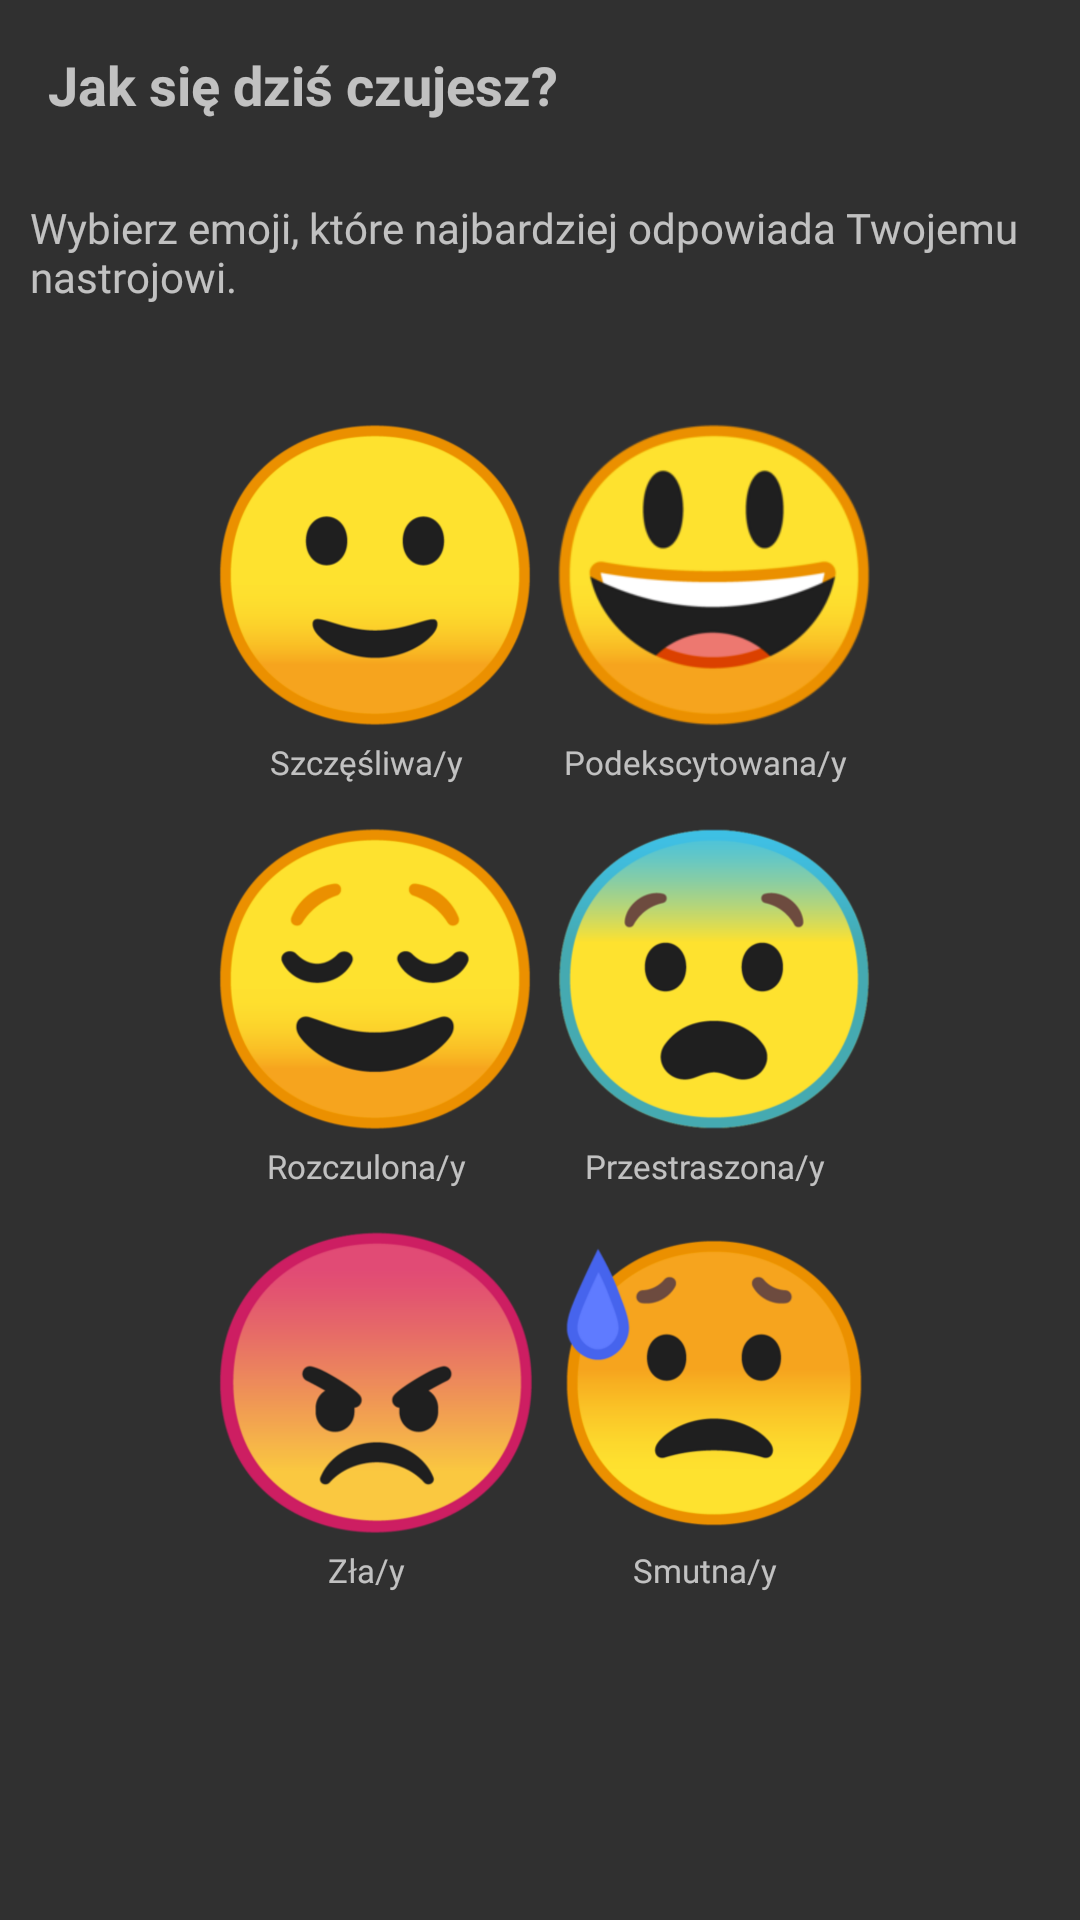
\includegraphics[scale=0.13]{rozdzial3/screen-emoji.png}
		\subcaption{\label{subfigure_a}}
	\end{subfigure}
	\begin{subfigure}{0.35\textwidth}
		\centering
		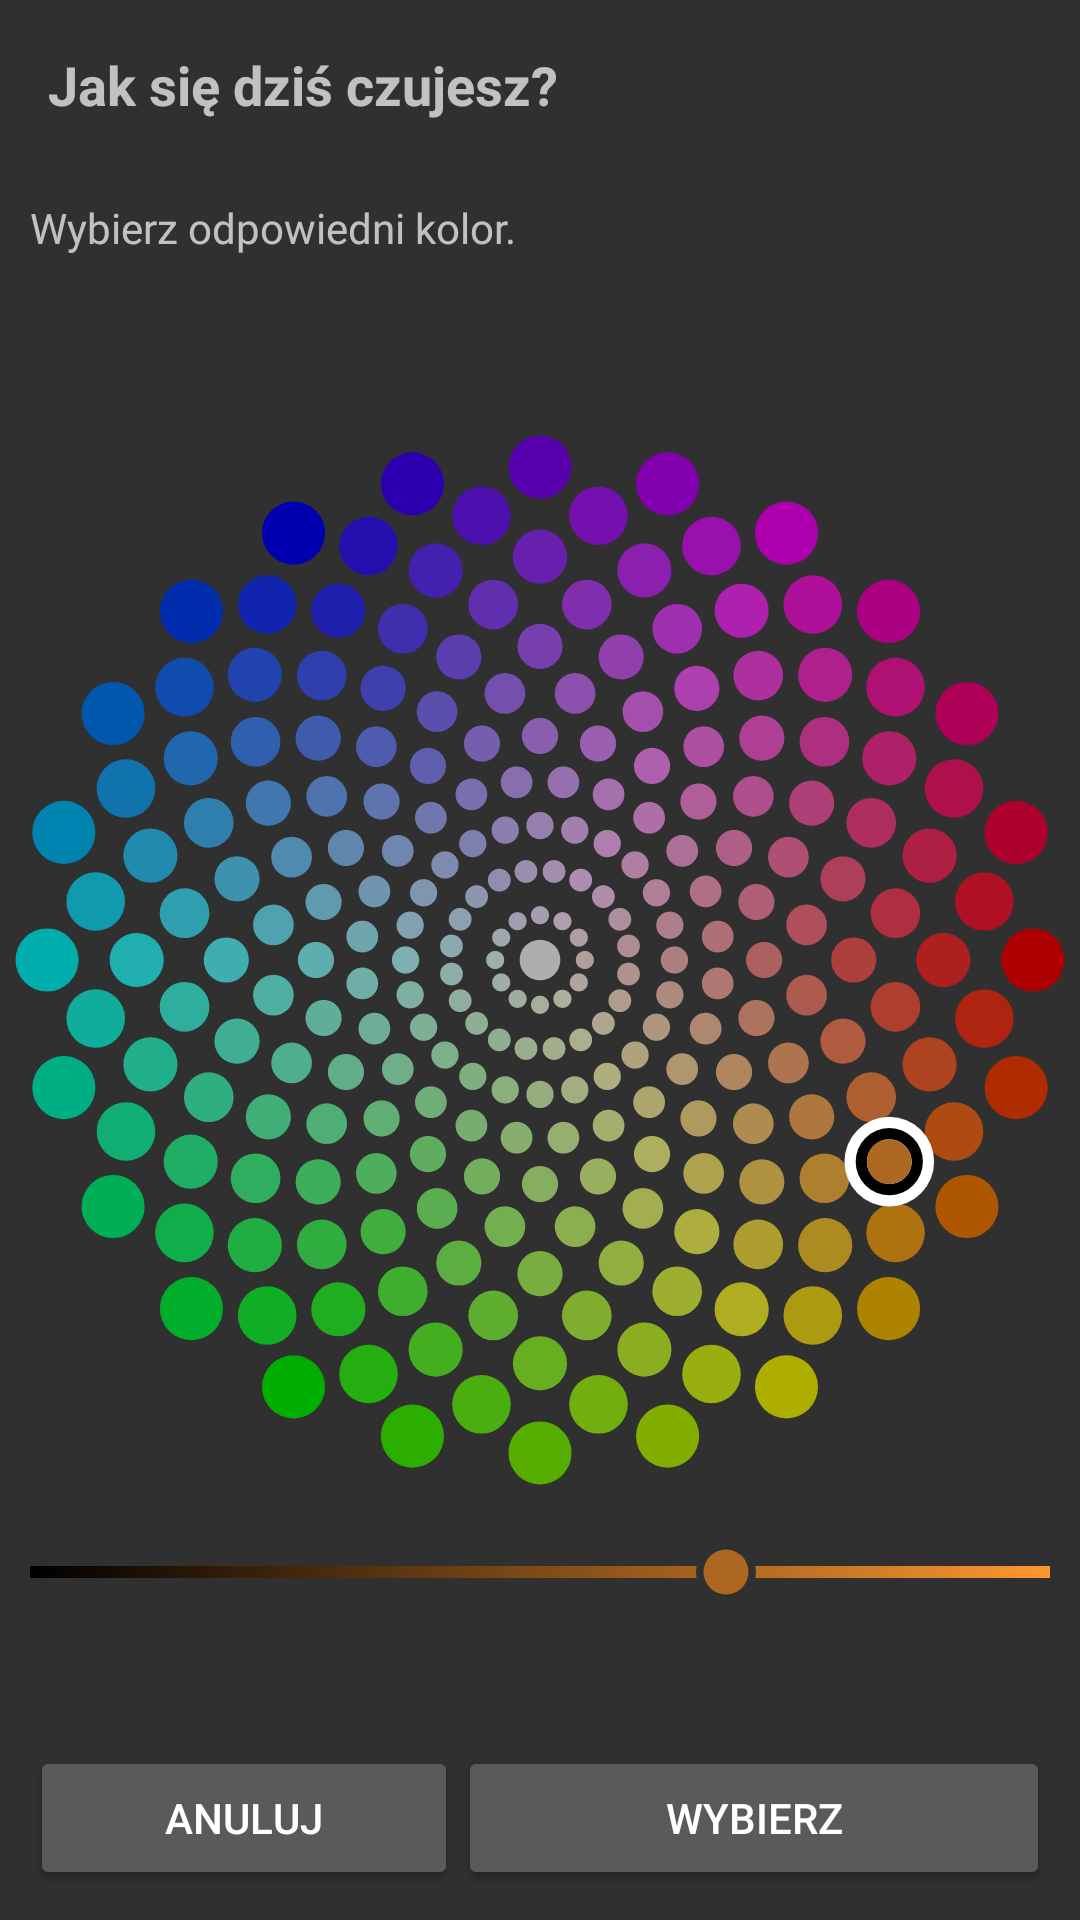
\includegraphics[scale=0.13]{rozdzial3/screen-color.png}
		\subcaption{\label{subfigure_b}}
	\end{subfigure}
	\caption{ Dialog z użytkownikiem w formie pytania o emocje (a) oraz pytania o kolory (b).}
\end{figure}


\subsection{Pakiet \textit{photo}}

W dwudziestym pierwszym wydaniu systemu Android, Google udostępniło deweloperom narzędzie, które pozwala kontrolować dostępne w smartfonie aparaty – \textit{android.hardware.camera2} API. Zaimplementowany w pluginie \textit{HowAreYou} pakiet \textit{photo} jest odpowiedzialny za wszytkie czynności potrzebne do wykonania zdjęcia „w tle”, to znaczy automatycznie, bez konieczności podglądu użytkownika, odpowiednim aparatem. Zdjęcia wykonywane są tylko i wyłącznie wtedy, gdy jest na to zgoda użytkownika.

\begin{figure}[H]
	\centering
	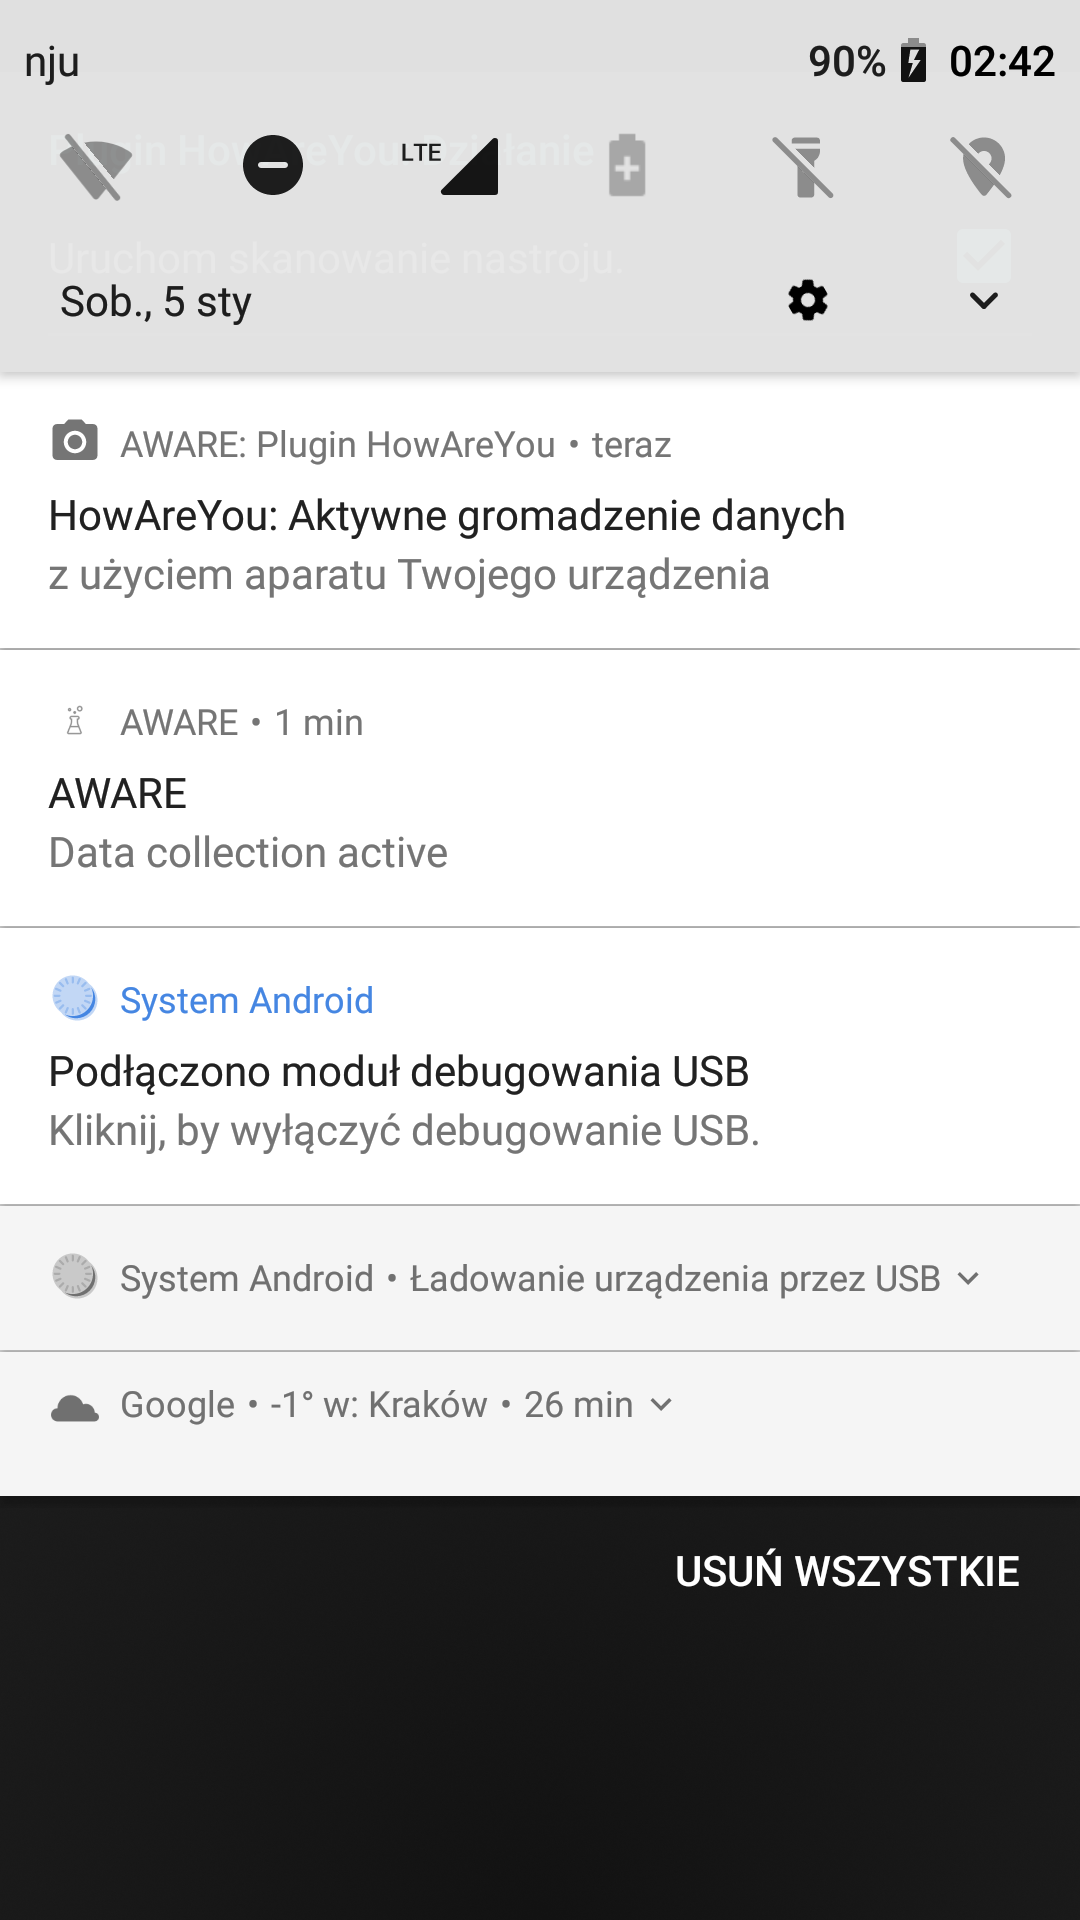
\includegraphics[scale=0.13]{rozdzial3/screen-background.png}
	\caption{Użytkownik może zdecydować, aby powiadomienie przypominało mu o możliwości rejestracji wizerunku.}
\end{figure}

Podobnie jak dialog z użytkownikiem, rozpoznawanie emocji z wykorzystaniem kamery telefonu zostało zrealizowane w pluginie od zera -- wykorzystując doświadczenie zdobyte w trakcie tworzenia aplikacji \textit{HowAreYou} i łącząc je z możliwościami frameworka \textit{AWARE}. Poprawiono wykorzystanie \textit{camera2 API}. Zdjęcia są teraz wyraźne i odpowiednio naświetlone. Fotografie robione są w tle, bez ingerencji w działanie użytkownika. W przypadku niepowodzenia wykrycia emocji proces może być powtórzony zadaną ilość razy w zadanym interwale.

Samo wykrywanie emocji składa się z dwóch etapów. W pierwszym etapie wykorzystywany jest \textit{FaceDetector} Google. Z jego pomocą plugin sprawdza obecność twarzy w kadrze zdjęciowym i dopiera najlepszą rotację zdjęcia dla dalszego procesowania. W dalszej części plik jest wysyłany do serwera \textit{MS face API} gdzie następuje rozpoznanie emocji. Informacja zwrotna zostaje zapisana w bazie \textit{SQLite}.


\subsection{Menu ustawień}


Aby uruchomic aktywność ustawień, w aplikacji klienckiej \textit{AWARE} w menu \textit{Plugins} należy wybrać \textit{HowAreYou}, a następnie \textit{Settings}. Po naciśnięciu przycisku oczom użytkownika ukaże się menu, za pomocą którego można konfigurować plugin. Z poziomu menu możliwe jest:

\begin{itemize}
	\item Całkowite wyłączenie i ponowne włączenie pluginu \textit{HowAreYou}.
	
	\item Włączenie/wyłączenie wykorzystania kamery. Ta opcja może być ważna dla osób, które cenią swoją prywatność. Dzięki niej mogą kontrolować, kiedy dokładnie wykonywane są fotografie.
	
	\item Włączenie/wyłączenie wyświetlania przypomnienia, gdy kamera jest aktywna. Jeżeli użytkownik bierze udział w krótkim badaniu, może nie być przyzwyczajony do tego, że jego kamera może być aktywna. Ikona aparatu na pasku powiadomień i powiadomienie po rozwinięciu górnego paska mogą mu o tym przypomnieć.
	
	\item Włączenie/wyłączenie odpytywania użytkownika z użyciem emotikon oraz kolorów. Odpytywanie można wyłączyć całkowicie. Można też zdecydować się na jedną z dwóch dostępnych opcji.
	
	\item Włączenie/wyłączenie trybu synchronizacji danych tylko przez wifi. Ilość danych do zsynchronizowania może być naprawdę niemała, dlatego taka opcja może być szczególnie przydatna dla osób, które nie dysponują dużym pakietem zbędnych gigabajtów.
	
	\item Wybranie między modelem A (zaawansowany model HMR, \textit{patrz: rozdział 4}), a modelem B (wersja uproszczona modelu). Przy instalacji wersji A (\textit{patrz: dodatek A}), domyślnie wybrany jest model A, przy wersji B - model B.
	
	\item Uruchomienie trybu debugowego. W trybie debugowym na ekranie urządzenia wyświetlają się w formie wiadomości \textit{Toast} lub okna dialogowego dodatkowe informacje dotyczące działania algorytmów w tle. Na dłuższą metę użytkowanie telefonu z \textit{HowAreYou} w trybie debugowym może być bardzo irytujące i dlatego jest niezalecane.
	
\end{itemize}

Z poziomu menu ustawień możemy też obserwować działanie aplikacji. Możliwe jest:

\begin{itemize}
	\item Uruchomienie logu z ostatniego wnioskowania. Taki log zawiera informacje, jakie zwraca silnik wnioskujący \textit{HeaRTDroid}. Dane są przetworzone z użyciem specjalnego parsera, aby można je było analizować w nieco bardziej przejrzystej formie.
	
	\item Uruchomie logu aplikacji. Użytkownik może śledzić kolejne akcje tak, jakby to robił patrząc w konsolę \textit{Logcat}. Widok umożliwia śledzenie aplikacji bez \textit{ADB}. Log samodzielnie się nie odświeża.
	
	\item Uruchomienie logu ostatnich akcji. Poza samą listą kolejnych akcji użytkownik ma do dyspozycji informację o znaku czasu ostatniej akcji każdego typu, o łącznej ilości akcji danego typu jaka została wykonana na urządzeniu, oraz o ilości akcji danego typu, która wykonała się w ciągu ostatnich 24 godzin.
\end{itemize}

Ostatnią z możliwości menu Ustawień jest opcja wymuszenia. Ręcznie można wymusić zapytanie o kolor, zapytanie o emocje, czy skanowanie emocji z wykorzystaniem kamery telefonu. Użytkownik może też wymusić synchronizację z zewnętrzną bazą danych. Mimo, że sama synchronizacja uruchamiana jest przez plugin regularnie, wzięto pod uwagę, że może pojawić się sytuacja, kiedy synchronizacja jest potrzebna natychmiast, na przykład podczas krótkiej chwili połączenia z siecią WiFi lub na zakończenie badania, aby nie stracić ostatnich wyników.

\begin{figure}[H]
	\centering
	\begin{subfigure}{0.35\textwidth}
		\centering
		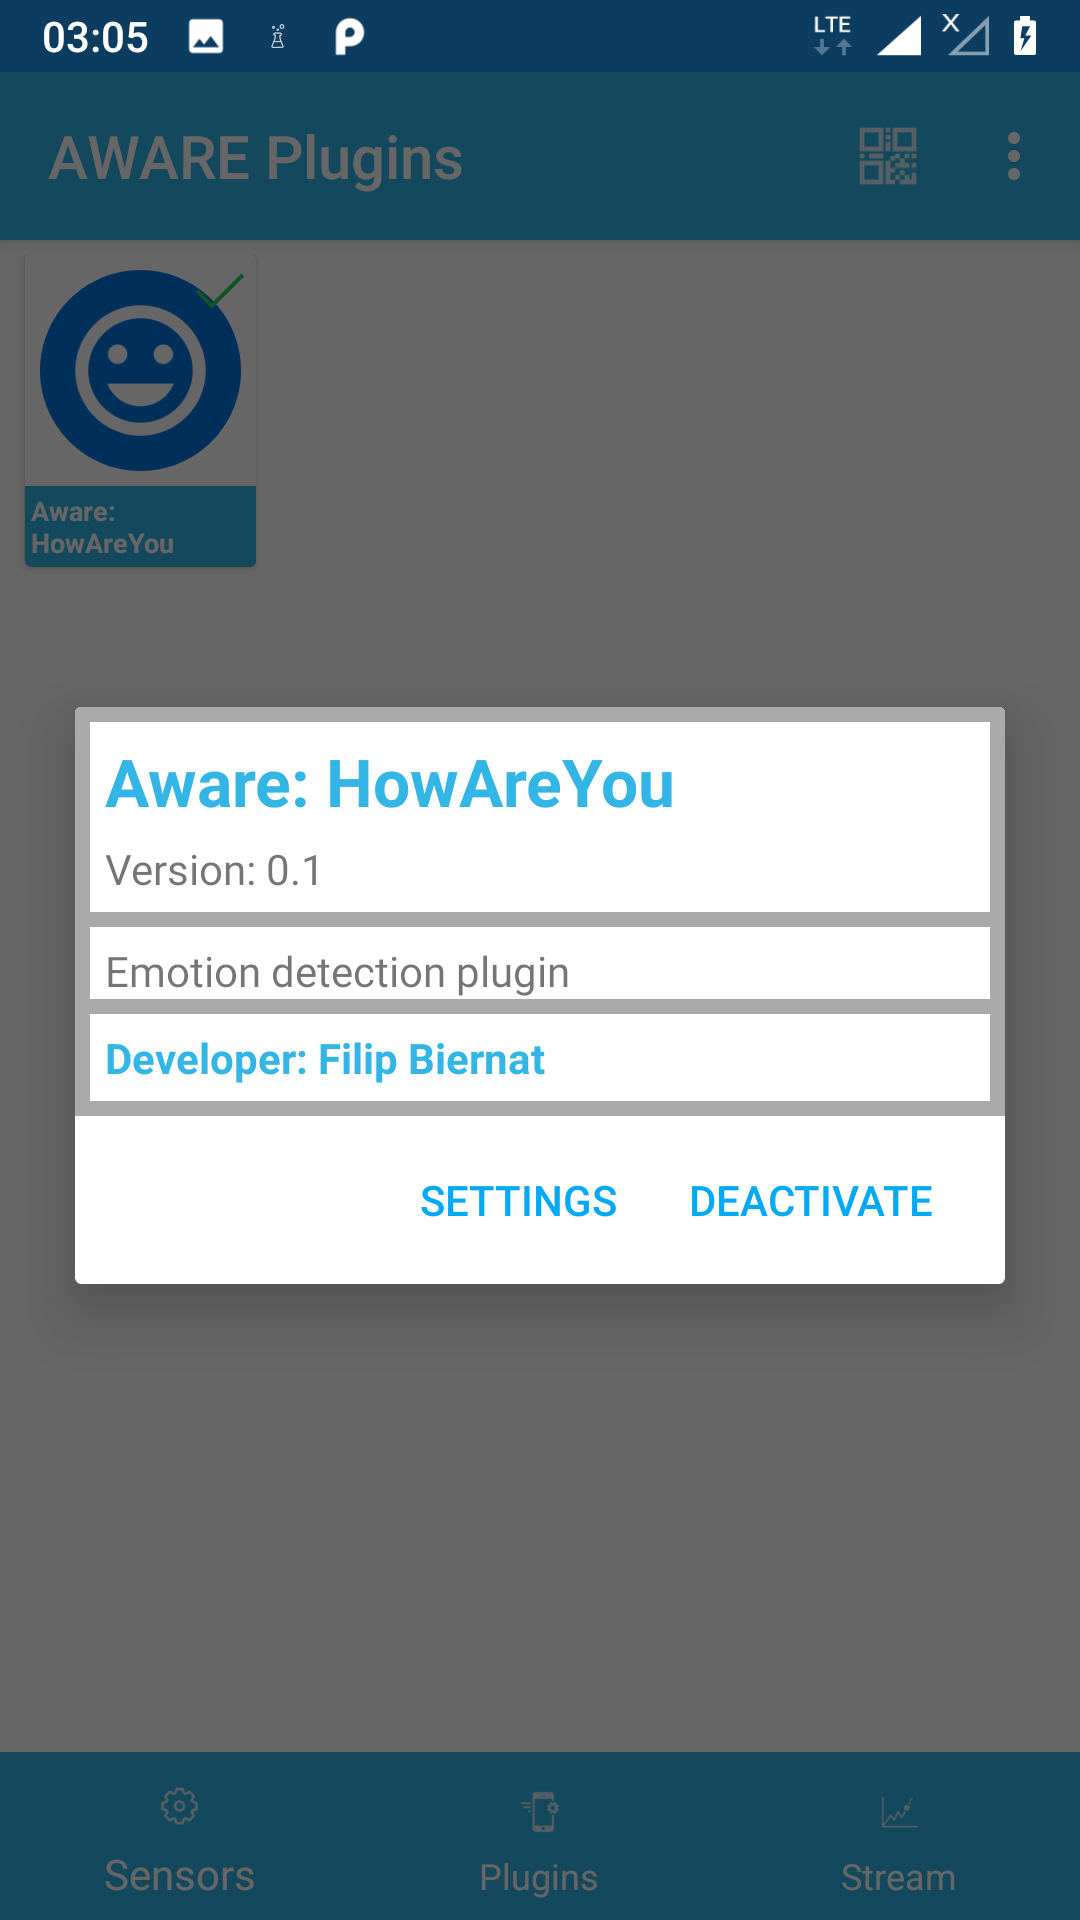
\includegraphics[scale=0.13]{rozdzial3/Ustawienia_uruchomienie.png}
		\subcaption{\label{subfigure_a}}
	\end{subfigure}
	\begin{subfigure}{0.35\textwidth}
		\centering
		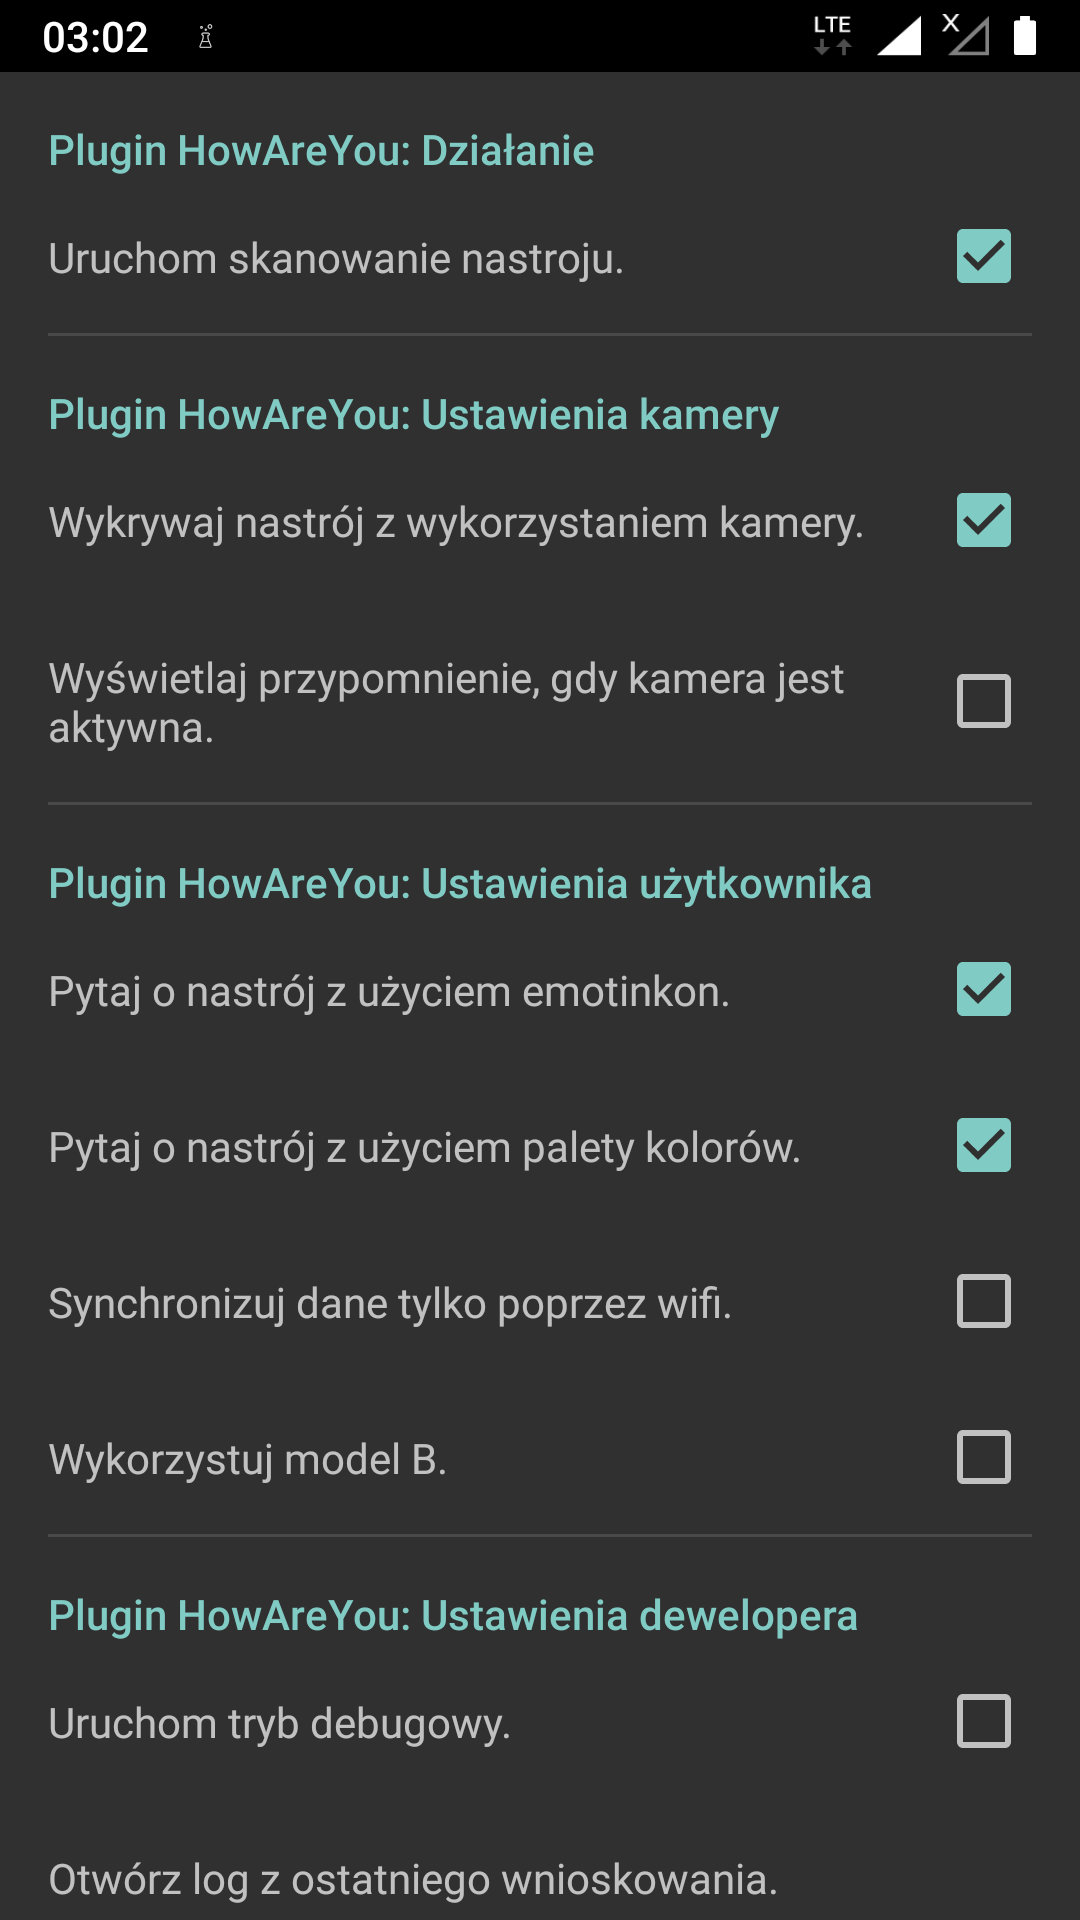
\includegraphics[scale=0.13]{rozdzial3/Ustawienia_cz1.png}
		\subcaption{\label{subfigure_b}}
	\end{subfigure}
	\caption{ Przejście do menu ustawień z aplikacji klienckiej (a) oraz widok aktywności ustawień (b).}
\end{figure}

\begin{figure}[H]
\centering
\begin{subfigure}{0.35\textwidth}
	\centering
	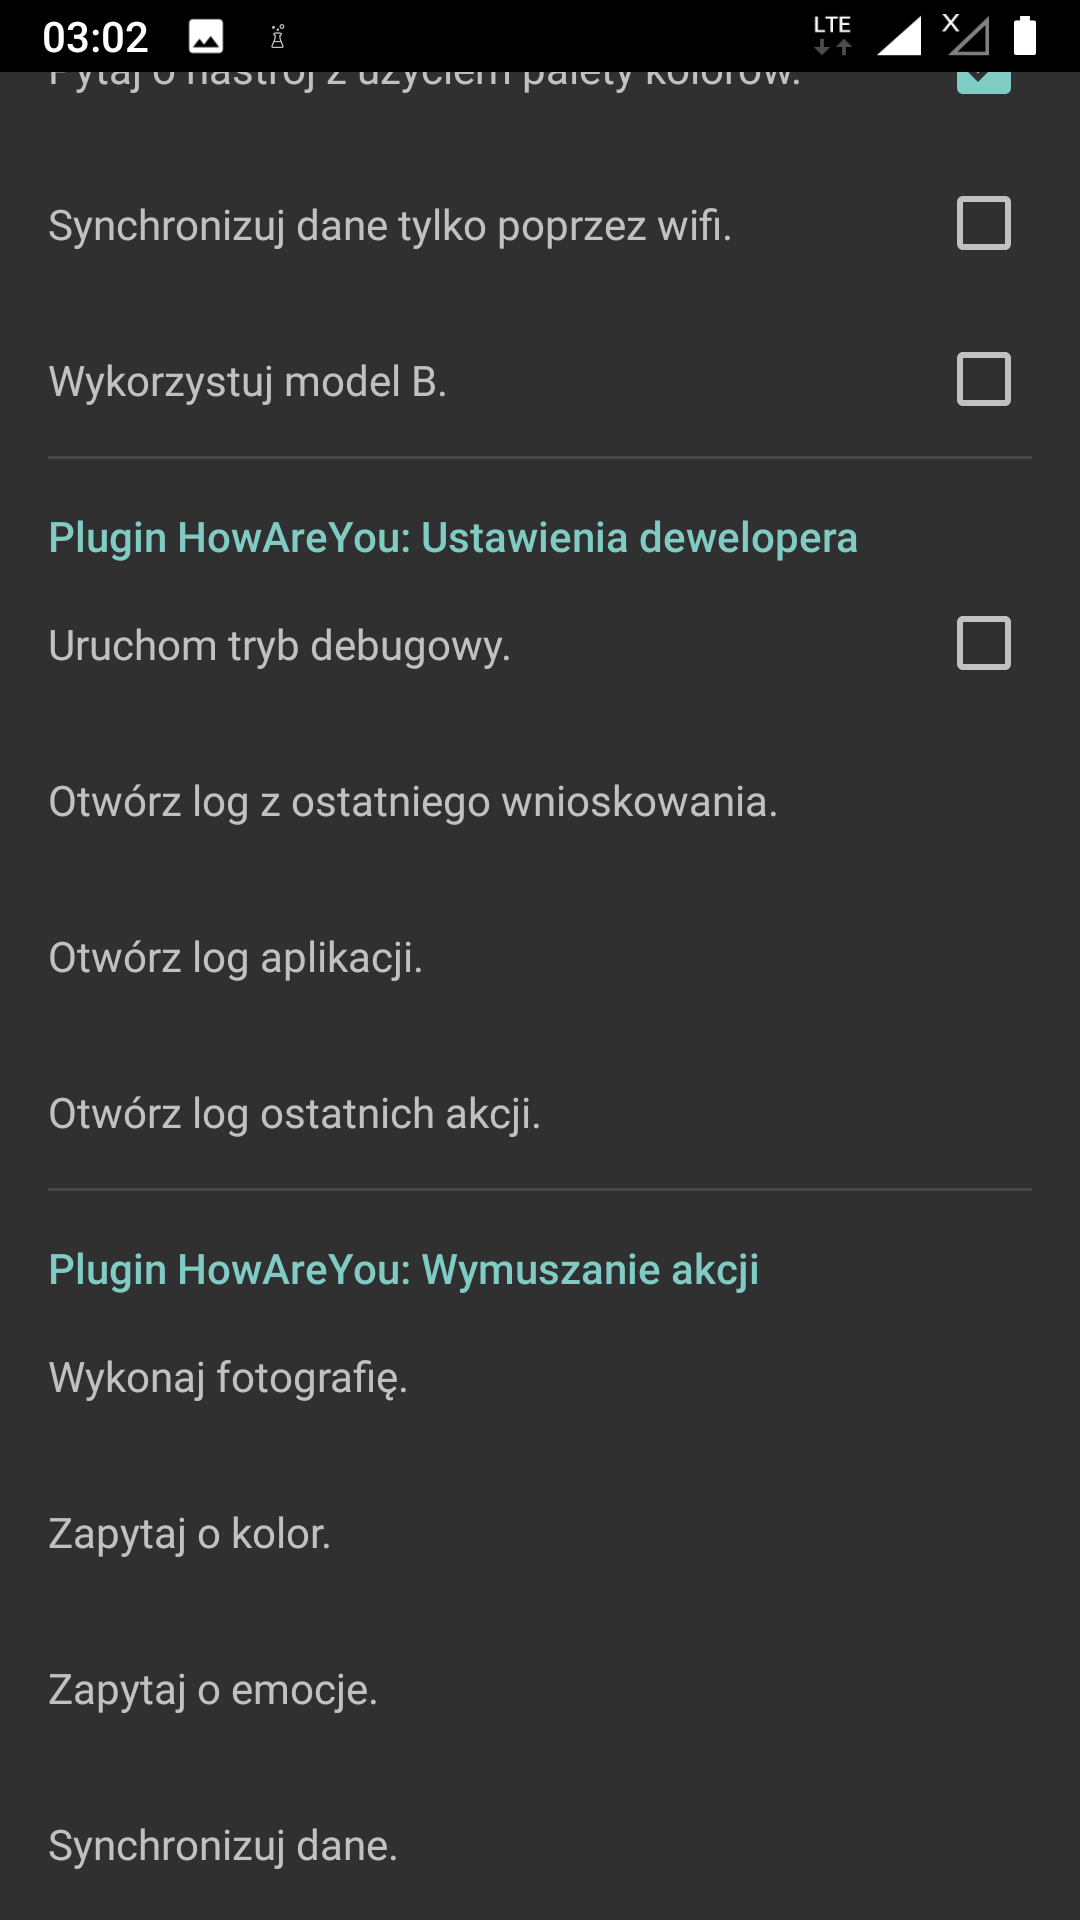
\includegraphics[scale=0.13]{rozdzial3/Ustawienia_cz2.png}
	\subcaption{\label{subfigure_a}}
\end{subfigure}
\begin{subfigure}{0.35\textwidth}
	\centering
	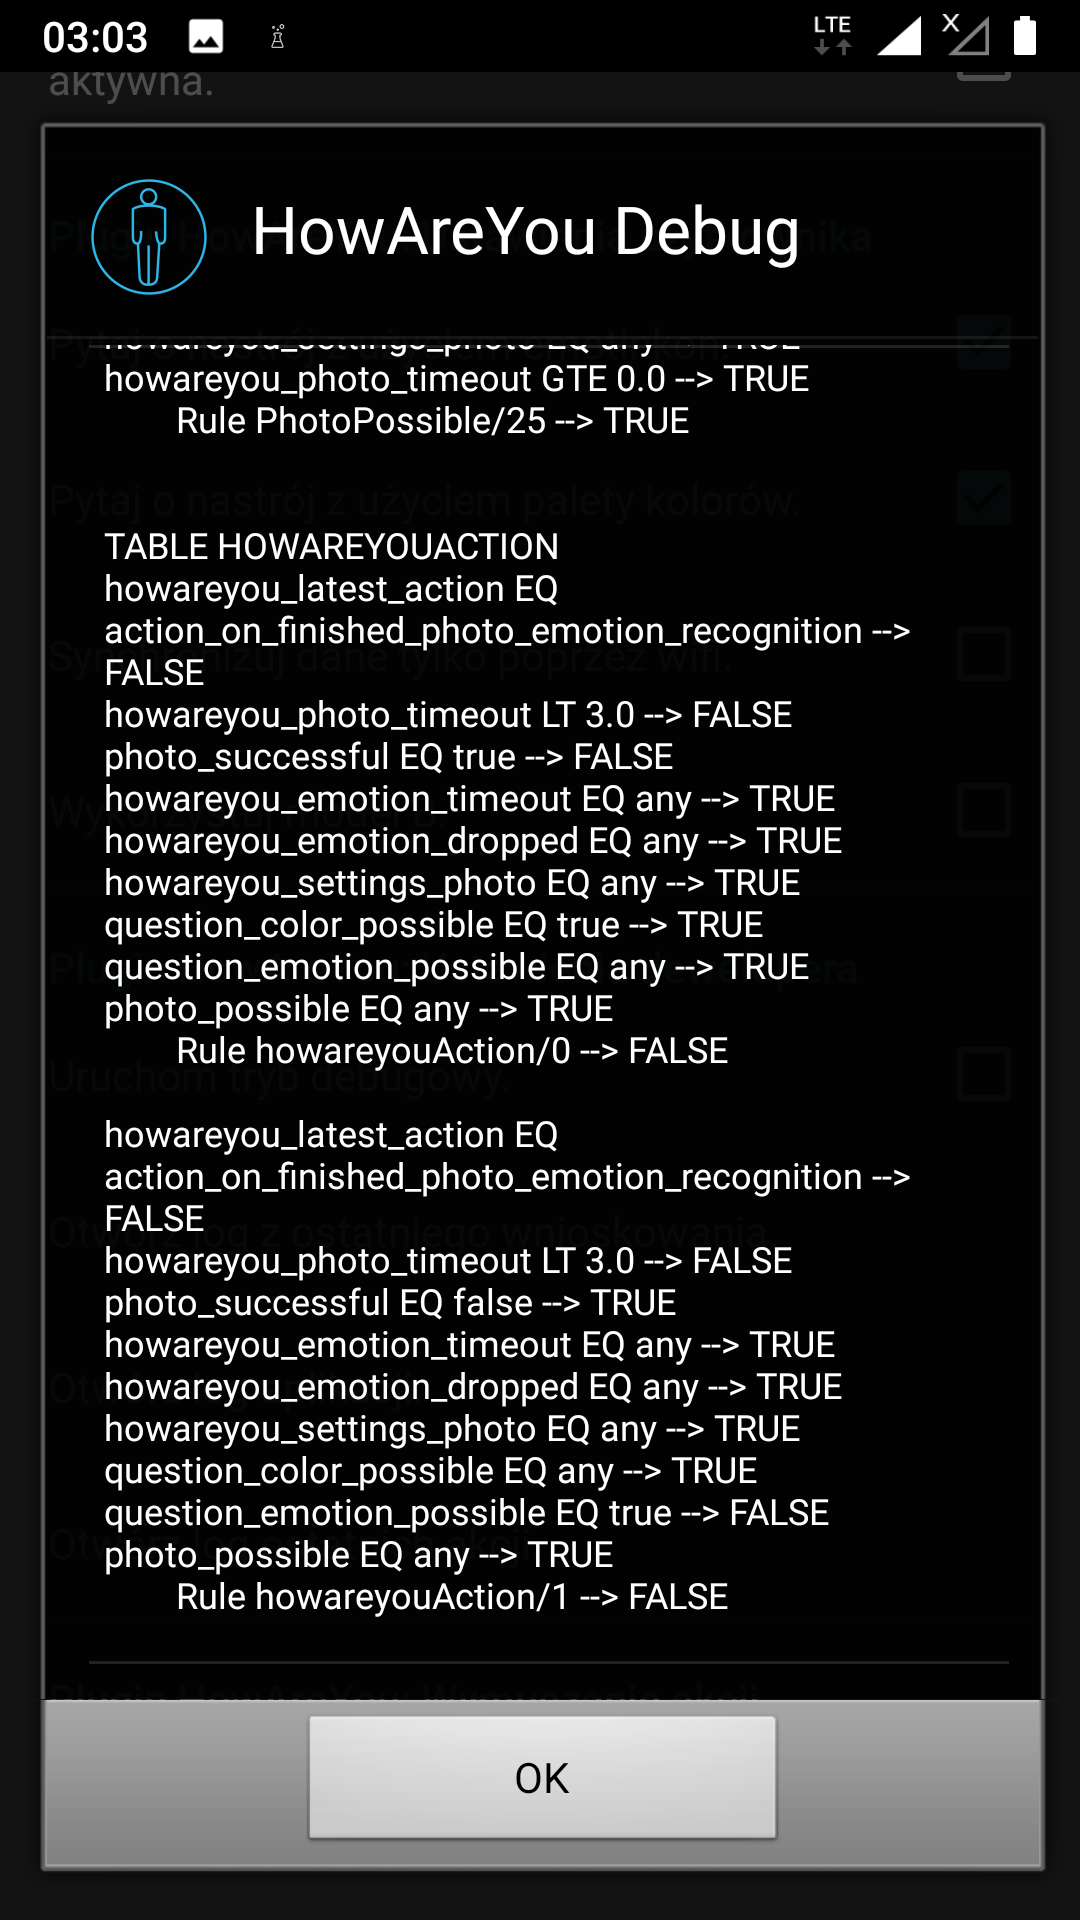
\includegraphics[scale=0.13]{rozdzial3/Ustawienia_logZWnioskowania.png}
	\subcaption{\label{subfigure_b}}
\end{subfigure}
\caption{ Widok dalszej części aktywności ustawień (a) oraz log z ostatniego wnioskowania (b).}
\end{figure}

\begin{figure}[H]
\centering
\begin{subfigure}{0.35\textwidth}
	\centering
	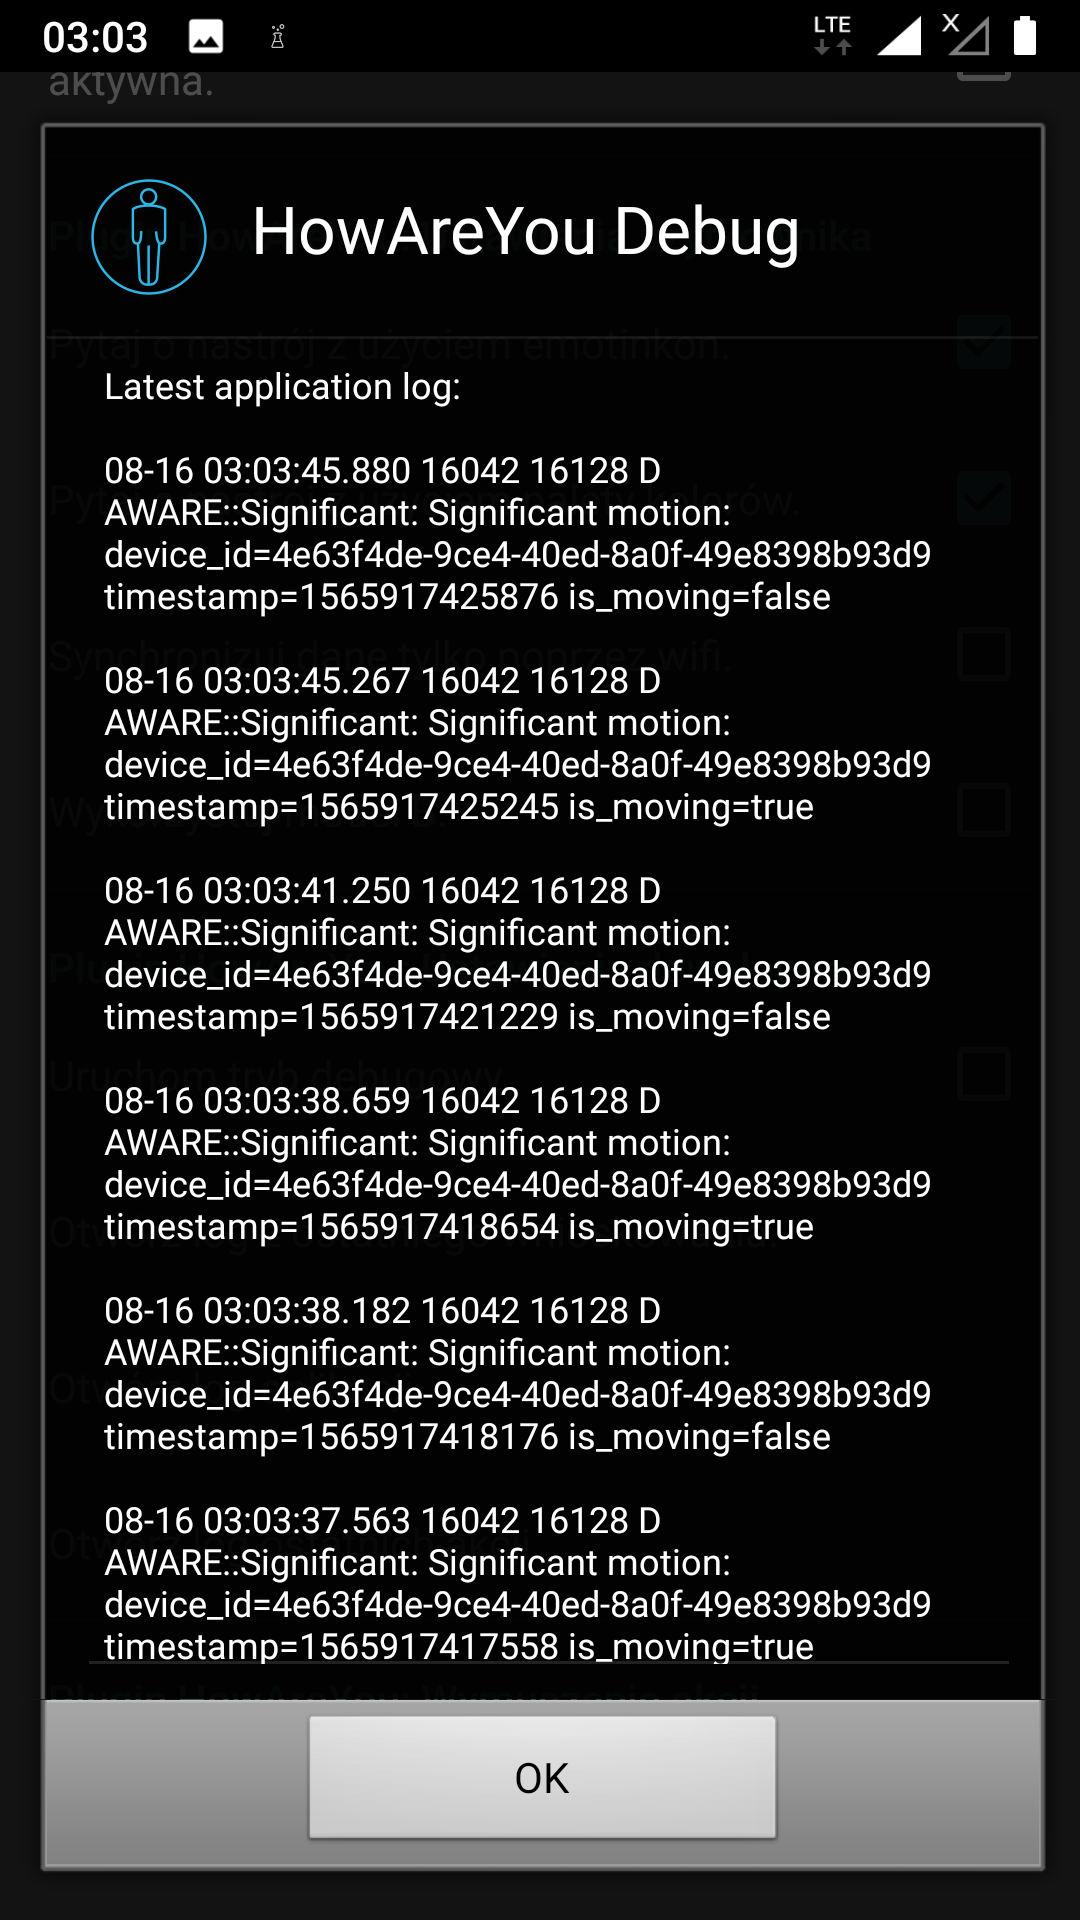
\includegraphics[scale=0.13]{rozdzial3/Ustawienia_logAplikacji.png}
	\subcaption{\label{subfigure_a}}
\end{subfigure}
\begin{subfigure}{0.35\textwidth}
	\centering
	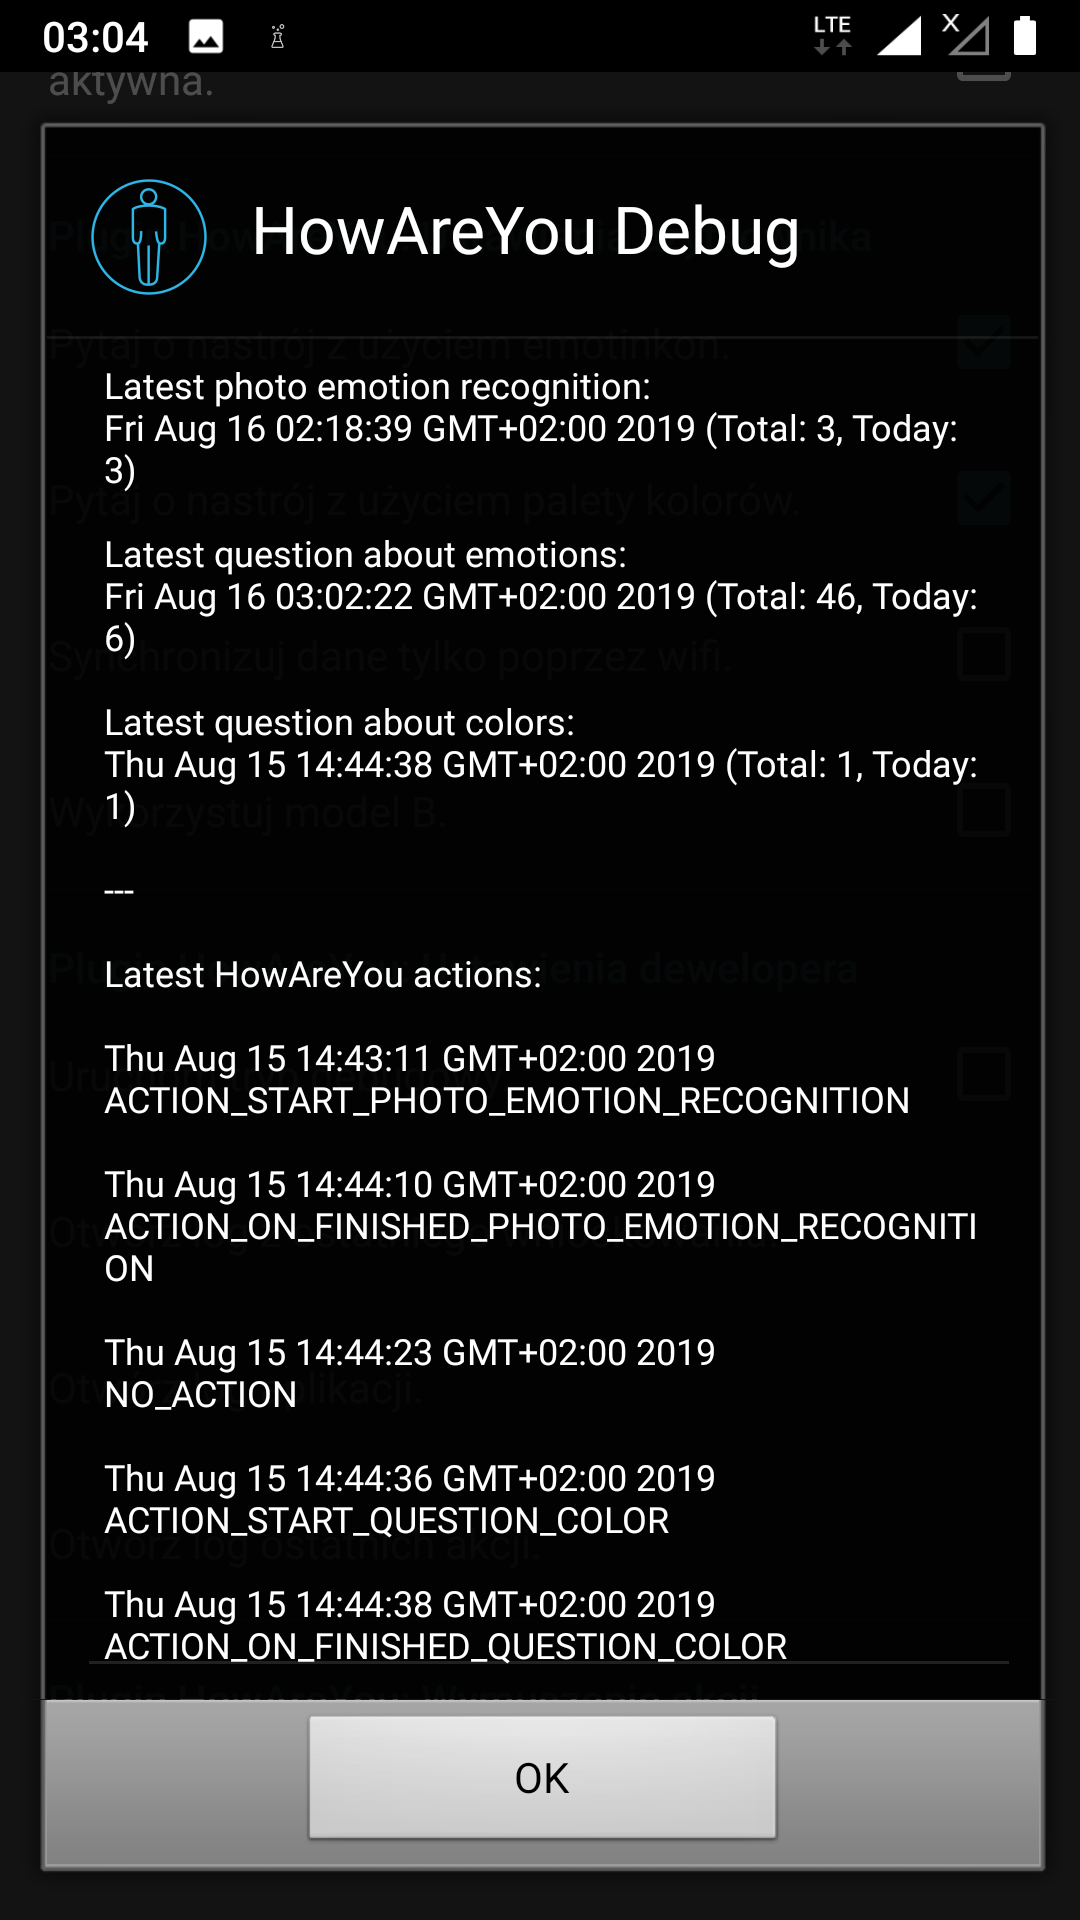
\includegraphics[scale=0.13]{rozdzial3/Ustawienia_logOstatnichAkcji.png}
	\subcaption{\label{subfigure_b}}
\end{subfigure}
\caption{ Log aplikacji \textit{HowAreYou} (a) oraz log ostatnich akcji (b).}
\end{figure}




	\chapter{Implementacja}
\label{cha:implementacja}

%---------------------------------------------------------------------------

\section{Wprowadzenie do implementacji}
\label{sec:wprowadzenieDoImplementacji}

Telefon komórkowy jest urządzeniem, które na co dzień mamy przy sobie. Z tego względu już na najwcześniejszym etapie projektowania rozwiązania wybór padł właśnie na to urządzenie. Jeżeli chodzi o systemy operacyjne, zdecydowano się na system Android. Jego główną zaletą jest fakt, że pozwala deweloperom aplikacji na szeroki dostęp do opcji systemowych, sensorów, itp. Jest to również najpopularniejszy system operacyjny dla urządzeń mobilnych.

Wraz z~potrzebą akwizycji dużej ilości różnego rodzaju danych z~sensorów urządzenia mobilnego pojawiła się konieczność realizacji tej akwizycji. Zdecydowano się pominąć własną implementację tego mechanizmu wykorzystując szeroki wachlarz możliwości jaki daje jeden z~otwartoźródłowych frameworków. Ostatecznie wybór padł na framework \textit{AWARE}. Rozwiązanie realizujące różne metody mediacji wiedzy zostało więc stworzone jako plugin \textit{HowAreYou} - nieoficjalne rozszerzenie \textit{AWARE}.

Implementacja pluginu została zrealizowana w~języku Java, rekomendowanym przez twórców frameworka \textit{AWARE}\cite{AwareFramework}. Najstarszą wersją systemu operacyjnego Android, jaką wspiera \textit{HowAreYuu} jest Lollipop (minimalne SKD zostało ustawione na 22). Środowiskiem wykorzystanym w~celu realizacji zadania było Android Studio. Do kontroli wersji wykorzystano narzędzie git, do przechowywania kodu źródłowego -- platformę github: \url{https://github.com/filipbiernat/HowAreYou_plugin}.

%---------------------------------------------------------------------------

\section{Model HMR}
\label{sec:modelHmr2}

\subsection{Konstruowanie modelu wnioskującego}

Do tworzenia pliku \textit{model.hmr} wykorzystana została aplikacja webowa \textit{HeaKatE Web Editor} (w~skrócie \textit{HWEd}). \textit{HWEd} jest edytorem online (stworzonym z~wykorzystaniem środowiska \textit{node.js}) służącym do tworzenia i edytowania modeli, które później wykorzystywane są przez silnik wnioskujący \textit{HeaRTDroid} \cite{heartdroid}. Zawarty w~nim parser przetwarza reguły \textit{XTT2} na czytelne dla użytkownika zestawy połączonych ze sobą tabel, a następnie po wybraniu opcji \textit{Export} przekształca tablice w~plik HMR z~regułami \textit{XTT2} \cite{heartdroid}.

Samo \textit{XTT2} jest formalizmem reprezentacji wiedzy stworzonym z~myślą o regułach. Służy algebraicznej i logicznej specyfikacji reguł pozwalając na zwięzły, przejrzysty i efektywny sposób wizualnej reprezentacji wiedzy. W odróżnieniu od tradycyjnych systemów pozwala wykorzystanie ,,płaskiego'' (jednoopoziomowego) zestawu reguł. Wprowadza tablice, wykorzystywane do reprezentowania zestawów reguł mających podobrą strukturę, oraz połączenia między tablicami. Struktura zestawów tabel przypomina drzewa decyzyjne \cite{AiWikiHekate}.

Podczas opracowywania modelu wykorzystane zostało również narzędzie \textit{HeaRTDroid Query Notation} (w skrócie \textit{HaQuNa}). \textit{HaQuNa} jest prostym językiem, który może być wykorzystywany w~interaktywnej powłoce. Zestaw poleceń linii komend umożliwia wczytywanie, modyfikację oraz uruchamianie modeli HMR\cite{heartdroid}. Przy implementacji \textit{HowAreYou} \textit{HaQuNa} była wykorzystywana do weryfikacji poprawności tworzonego modelu.

Należy jeszcze podkreślić, że model HMR został architektonicznie oddzielony od implementacji aplikacji. Dzięki zastosowaniu tego rozwiązania, plugin \textit{HowAreYou} nie musi być powiązany z~obecnie zaimplementowanym domyślnym modelem. Ekspert domenowy, który nie musi być nawet osobą techniczną, może bez trudu z~wykorzystaniem edytora online stworzyć nowy zestaw reguł \textit{XTT2} i zastąpić w~strukturze projektu plik \textit{model.hmr}.

\subsection{Zaawansowany model wnioskujący}

\subsubsection{Realizacja zaawansowanego modelu wnioskującego}

Celem realizacji zaawansowanego modelu wnioskującego było opracowanie modelu, z~pomocą którego zostaną wybrane jak najlepszy moment i sposób na zapytanie użytkownika o jego samopoczucie. Możliwe jest zapytanie niejawne poprzez wykonanie i przetworzenie fotografii lub zapytanie jawne - o kolor lub bezpośrednio o emocje.

W procesie wnioskowania brane są pod uwagę czynniki takie jak czas, który upłynął od ostatniego zapytania, korzystanie z~nawigacji samochodowej, wykonywanie połączenia telefonicznego, oglądanie filmów, czy wykonywanie ruchu. Uwzględniane są też wyniki analizy fotografii oraz wiedza, czy w~danej chwili użytkownik korzysta z~ekranu telefonu.

Poniższe obrazy przedstawiają widok modelu HMR w~edytorze \textit{HWEd}. Model został skonstruowany jako zestaw tabel, które zależąc od informacji z~aplikacji oraz od siebie nawzajem realizują reguły decyzyjne. Decyzja z~jednej tabeli ma bezpośreni wpływ na działanie kolejnej. Ostatecznie zgodnie z~wynikiem z~ostatniej tabeli \textit{howareyouAction} plugin \textit{HowAreYou} podejmuje określoną akcję. W kolejnej części rozdziału omawiane zostają krok po kroku zasady działania poszczególnych tabel poniższego modelu.

\begin{figure}[H]
	\centering
	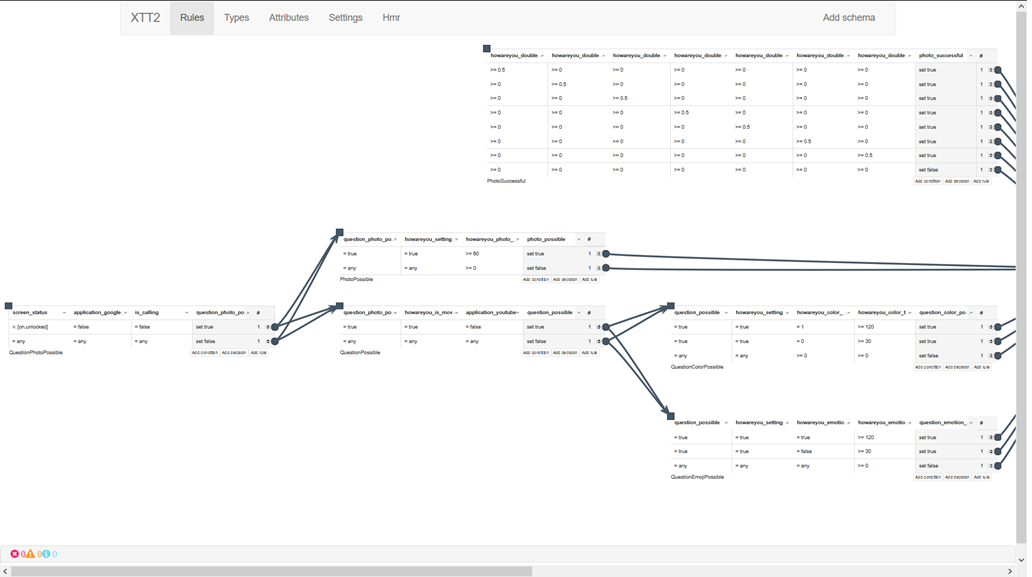
\includegraphics[scale=0.75]{rozdzial4/HMR_advancedModelPart1.png}
	\caption{Zaawansowany model wnioskujący: część 1.}
\end{figure}

\begin{figure}[H]
	\centering
	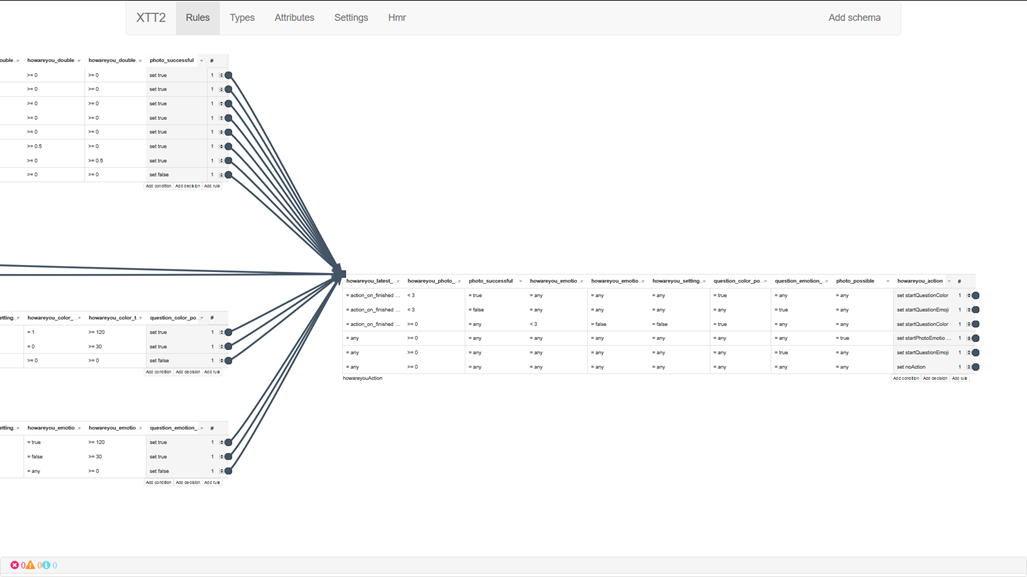
\includegraphics[scale=0.75]{rozdzial4/HMR_advancedModelPart2.png}
	\caption{Zaawansowany model wnioskujący: część 2.}
\end{figure}


\subsubsection{Tabela QuestionPhotoPossible}

Tabela zwraca prawdę, jeżeli spełnione są wspólne warunki konieczne do zapytania użytkownika lub wykonania zdjęcia.

Żeby uruchomić pytanie lub zrobić zdjęcie ekran telefonu musi być aktywny, telefon nie może prowadzić nawigacji, ani wykonywać połączenia.

\begin{figure}[H]
	\centering
	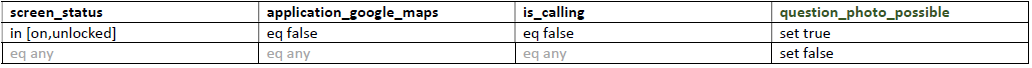
\includegraphics[scale=0.75]{rozdzial4/HMR_QuestionPhotoPossible.png}
	\caption{Zaawansowany model wnioskujący: tabela QuestionPhotoPossible.}
\end{figure}


\subsubsection{Tabela PhotoPossible}

Tabela zwraca prawdę, jeżeli spełnione są warunki konieczne do wykonania zdjęcia.

Żeby zrobić zdjęcie telefon musi spełniać warunki konieczne wspólne dla zdjęcia i pytania. Dodatkowo opcja wykonywania zdjęć musi być uruchomiona i czas, jaki upłynął od ostatniego zdjęcia, musi być większy lub równy 60 minut.

\begin{figure}[H]
	\centering
	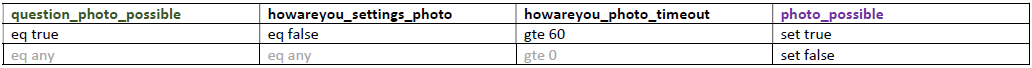
\includegraphics[scale=0.75]{rozdzial4/HMR_PhotoPossible.png}
	\caption{Zaawansowany model wnioskujący: tabela PhotoPossible.}
\end{figure}


\subsubsection{Tabela QuestionPossible}

Tabela zwraca prawdę, jeżeli spełnione są warunki konieczne do zapytania użytkownika.

Żeby uruchomić pytanie telefon musi spełniać warunki konieczne wspólne dla zdjęcia i pytania. Dodatkowo musi znajdować się w~ruchu (jeżeli jest w~bezruchu, najprawdopodobniej jest odłożony) i nie może być uruchomiona aplikacja do oglądania filmów. 

\begin{figure}[H]
	\centering
	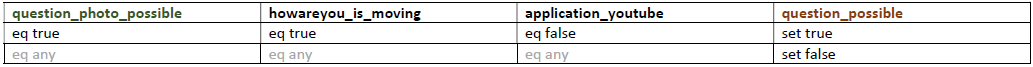
\includegraphics[scale=0.75]{rozdzial4/HMR_QuestionPossible.png}
	\caption{Zaawansowany model wnioskujący: tabela QuestionPossible.}
\end{figure}


\subsubsection{Tabela QuestionColorPossible}

Tabela zwraca prawdę, jeżeli spełnione są warunki konieczne do zapytania użytkownika o kolor.

Żeby uruchomić pytanie o kolor telefon musi spełniać warunki konieczne do zadania pytania. Dodatkowo ustawienia pluginu muszą pozwalać zapytać o kolor. Jeżeli ostatnie pytanie o kolor było odrzucone, kolejne pytanie może być zadane po 120 minutach. Jeżeli nie było odrzucone – po 30 minutach.

\begin{figure}[H]
	\centering
	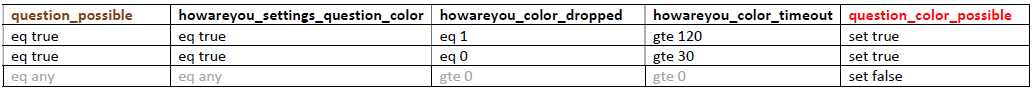
\includegraphics[scale=0.75]{rozdzial4/HMR_QuestionColorPossible.png}
	\caption{Zaawansowany model wnioskujący: tabela QuestionColorPossible.}
\end{figure}


\subsubsection{Tabela QuestionEmojiPossible}

Tabela zwraca prawdę, jeżeli spełnione są warunki konieczne do zapytania użytkownika o emocje.

Żeby uruchomić pytanie o emocje telefon musi spełniać warunki konieczne do zadania pytania. Dodatkowo ustawienia pluginu muszą pozwalać zapytać o emocje. Jeżeli ostatnie pytanie o emocje było odrzucone, kolejne pytanie może być zadane po 120 minutach. Jeżeli nie było odrzucone – po 30 minutach.

\begin{figure}[H]
	\centering
	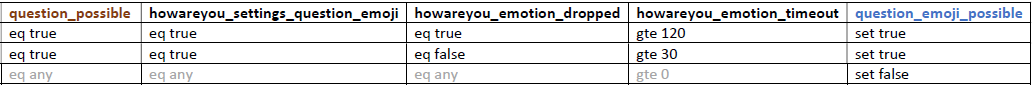
\includegraphics[scale=0.75]{rozdzial4/HMR_QuestionEmojiPossible.png}
	\caption{Zaawansowany model wnioskujący: tabela QuestionEmojiPossible.}
\end{figure}


\subsubsection{Tabela PhotoSuccessful}

Tabela zwraca prawdę, jeżeli najnowsze zdjęcie w~bazie danych uznaje się za udane.

Żeby uznać zdjęcie za udane wystarczy, że wartość prawdopodobieństwa jednej z~wykrytych emocji (za wyjątkiem emocji \textit{neutral}) jest większa niż próg (który obecnie wynosi 50 procent pewności).

\begin{figure}[H]
	\centering
	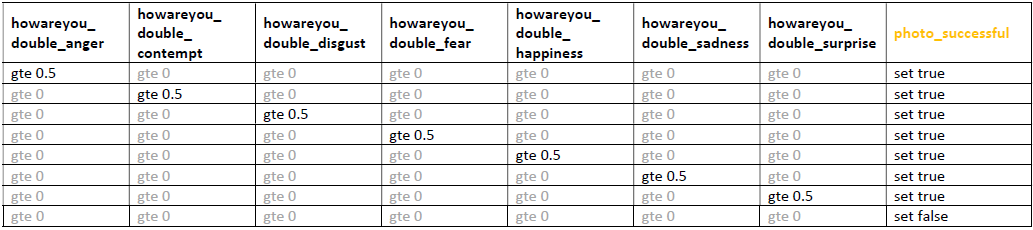
\includegraphics[scale=0.75]{rozdzial4/HMR_PhotoSuccessful.png}
	\caption{Zaawansowany model wnioskujący: tabela PhotoSuccessful.}
\end{figure}


\subsubsection{Tabela howareyouAction}

Tabela zwraca prawdę, jeżeli najnowsze zdjęcie w~bazie danych uznaje się za udane. 
\begin{enumerate}
	\item Jeżeli ostatnią akcją jaką plugin wykonał było zdjęcie i to zdjęcie było niedawno (mniej niż 3 minuty temu) i to zdjęcie było udane, to telefon zapyta o kolor, jeżeli spełnione są warunki do zapytania o kolor.
	\item Jeżeli ostatnią akcją jaką plugin wykonał było zdjęcie i to zdjęcie było niedawno (mniej niż 3 minuty temu), ale nie było udane, to telefon zapyta o emocje, jeżeli spełnione są warunki do zapytania o emocje.
	\item Jeżeli ostatnią akcją jaką plugin wykonał było pytanie o emocje i to pytanie o emocje było niedawno (mniej niż 3 minuty temu) i użytkownik odpowiedział na to pytanie, to telefon zapyta o kolor, jeżeli spełnione są warunki do zapytania o kolor. Ta reguła (de facto dwa pytania jedno po drugim) wykona się tylko wtedy, gdy użytkownik w~ustawieniach wyłączył wykonywanie zdjęć. 
	\item Jeżeli jest możliwe zrobienie zdjęcia, to telefon wykona zdjęcie. 
	\item Jeżeli nie jest możliwe zrobienie zdjęcia, to telefon zapyta o emocje, jeżeli spełnione są warunki do zapytania o emocje.
	\item Jeżeli żadna z~akcji nie jest możliwa, telefon nie wykona akcji.
\end{enumerate}

\begin{figure}[H]
	\centering
	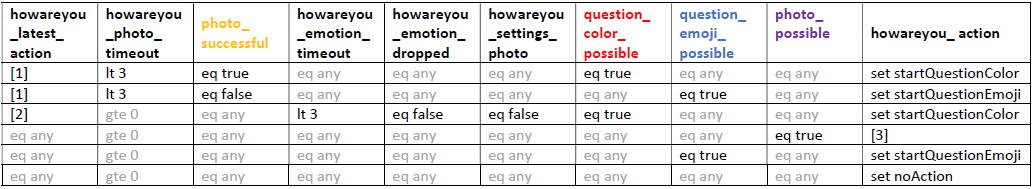
\includegraphics[scale=0.75]{rozdzial4/HMR_howareyouAction.png}
	\caption{Zaawansowany model wnioskujący: tabela howareyouAction.}
\end{figure}


\subsubsection{Obserwowanie reguł wnioskujących}

Działanie systemu wnioskującego wykorzystującego zaawansowany model wnioskujący można obserwować na bieżąco z~wykorzystaniem trybu debugowego. Po wybraniu opcji \textit{Otwórz log z~ostatniego wnioskowania} w~ustawieniach pluginu \textit{HowAreYou}, oczom użytkownika ukaże się okno ze szczegółowym opisem elementów wnioskowania: tabel, reguł i decyzji, jakie zostały podjęte.

\begin{figure}[H]
	\centering
	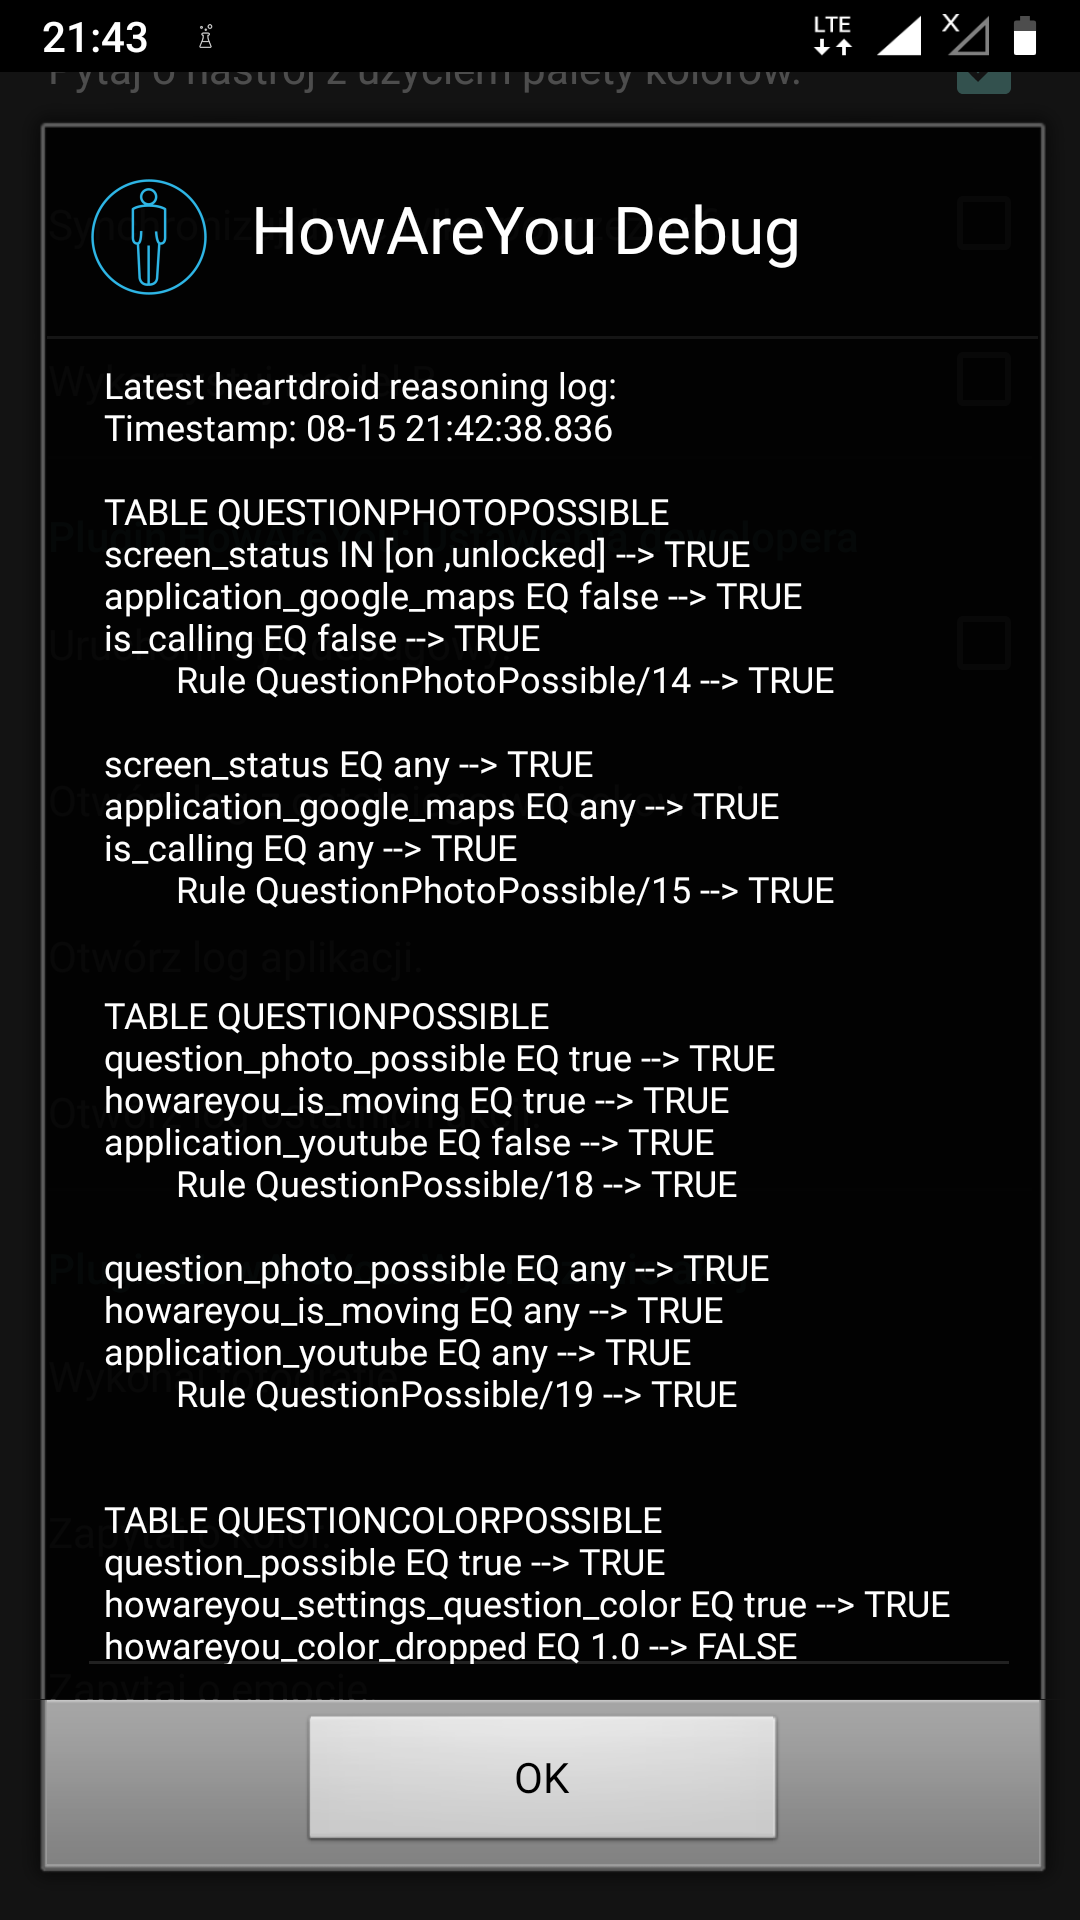
\includegraphics[scale=0.15]{rozdzial4/HMR_screenshots_A.png}
	\caption{Tryb debugowy: widok z~fragmentem loga z~wnioskowania HMR.}
\end{figure}



\subsection{Uproszczony model wnioskujący}


\subsubsection{Realizacja uproszczonego modelu wnioskującego}

W celach badawczych został stworzony również model uproszczony. Dzięki niemu osoba przeprowadzająca badanie jest w~stanie porównać, jaki wpływ na odbieranie przez uczestnika uciążliwości badania ma złożoność samego modelu. Model prosty został stworzony w~kontraście do pierwszego modelu. Sam model wykorzystuje tylko 2 czynniki: wiedzę czy ekran jest urządzenia włączony oraz czas od ostatniego zapytania. Model  symuluje prosty i toporny system odpytywania użytkownika. 

Zdecydowaną zaletą \textit{HowAreYou} jest fakt, iż w~celach porównawczych nie było niezbędne tworzenie dodatkowej aplikacji, która odpytywałaby użytkownika w~sposób uproszczony, ani nawet modyfikacja kodu źródłowego aplikacji. Jedyną potrzebną czynnością była zmiana samego modelu HMR. Model uproszczony można aktywować w~ustawieniach aplikacji. Można również zainstalować plugin \textit{HowAreYou} bezpośrednio z~modelem uproszczonym. Podczas pobierania pliku instalatora należy wybrać wersję B (\textit{patrz: dodatek A}).


\subsubsection{Tabela howareyouAction}

Tabela zwraca prawdę, jeżeli najnowsze zdjęcie w~bazie danych uznaje się za udane. 
\begin{enumerate}
	\item Jeżeli ekran urządzenia jest aktywny i od ostatniego zapytania minęło co najmniej 60 minut, aplikacja zapyta użytkownika o emocje.
	\item Jeżeli któryś z~powyższych warunków nie jest spełniony, telefon nie wykona żanej akcji.
\end{enumerate}

\begin{figure}[H]
	\centering
	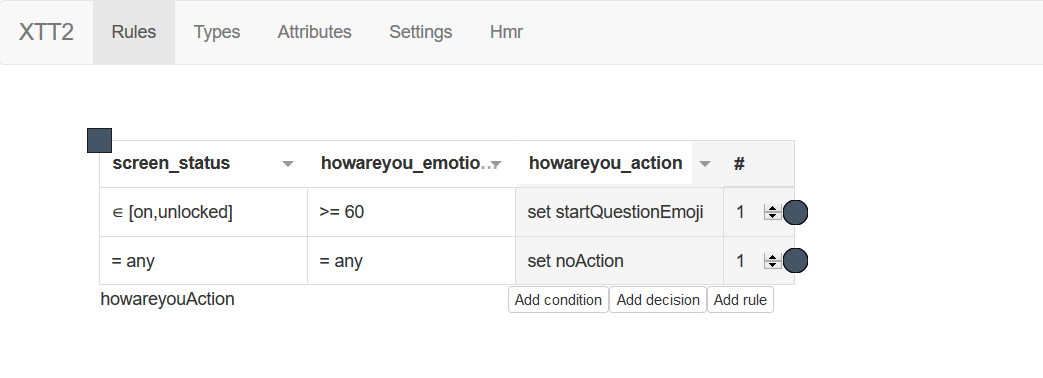
\includegraphics[scale=0.8]{rozdzial4/HMR_basic.png}
	\caption{Uproszczony model wnioskujący: tabela howareyouAction.}
\end{figure}

\subsubsection{Obserwowanie reguł wnioskujących}

Podobnie jak w~przypadku zaawansowanego modelu, działanie systemu wnioskującego wykorzystującego uproszczony model można obserwować na bieżąco z~wykorzystaniem trybu debugowego. Tutaj jednak log z~wnioskowania jest znacznie krótszy - do tego stopnia, że obejmuje tylko jedną tabelę i tylko dwie reguły.

\begin{figure}[H]
	\centering
	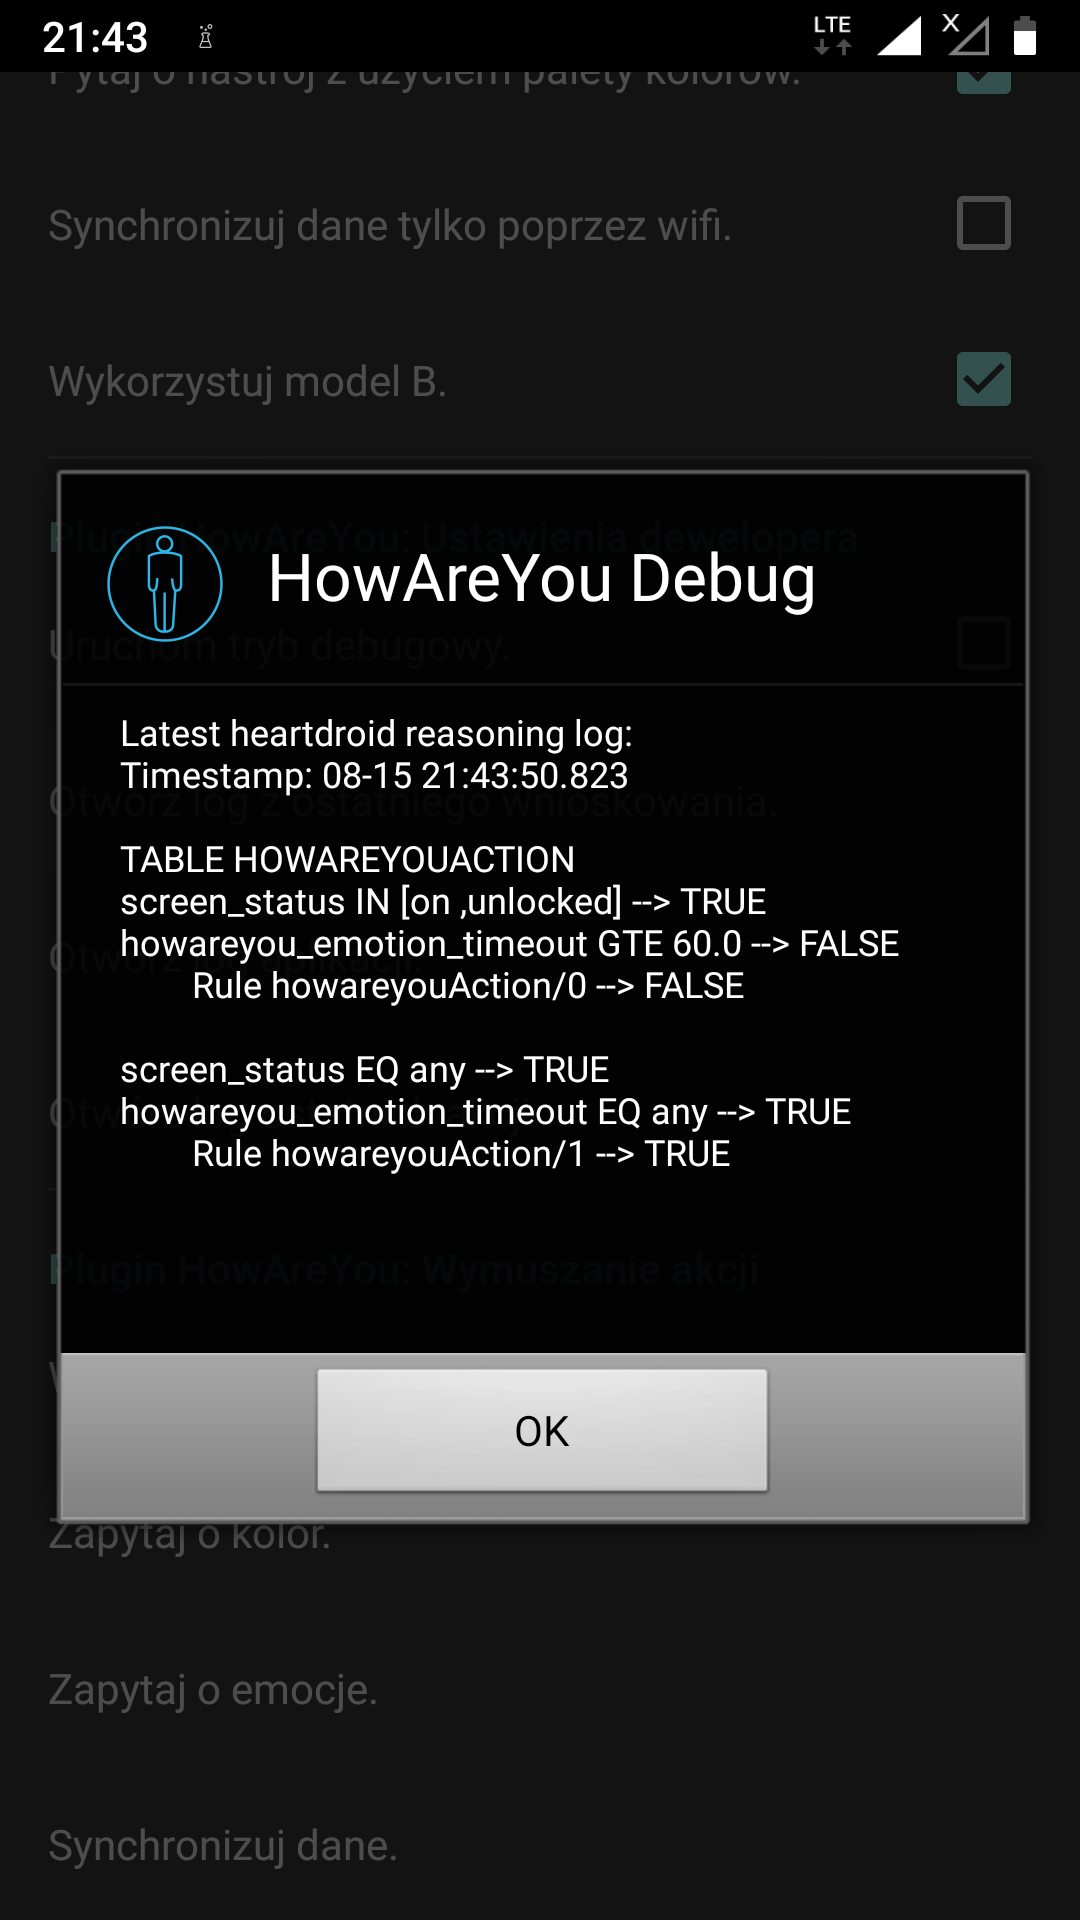
\includegraphics[scale=0.15]{rozdzial4/HMR_screenshots_B.png}
	\caption{Tryb debugowy: widok z~loga z~wnioskowania HMR z~modelem uproszczonym.}
\end{figure}

%---------------------------------------------------------------------------

\section{Pakiet \textit{HeaRT-AWARE}}
\label{sec:pakietHeartAware2}

Jak już wspomniano w~poprzednim rozdziale, zadaniem pakietu \textit{agh.heart} było zintegrowanie ze sobą frameworka \textit{AWARE} i silnika wnioskującego \textit{HeaRTDroid}. Zostało ono zaprojektowane przez autora pakietu w~formie trzech pomniejszych specjalistycznych pakietów: \textit{actions}, \textit{observers} i \textit{callbacks}\cite{heartaware}.

\subsection{Pakiet \textit{agh.heart.actions}}

W pluginie \textit{HowAreYou} zrezygnowano z~dostępnych początkowo w~pakiecie akcji \textit{DisableBlueTooth} (ang. wyłącz Bluetooth) i \textit{EnableBlueTooth} (ang. włącz Bluetooth). Przy realizacji aplikacji monitorującej nastrój użytkownika nie było potrzeby wykorzystywania tego typu akcji. W zamian zaimplementowano akcje związane ze specyfiką zadania:

\begin{itemize}
	\item \textit{HowAreYou\_StartPhotoEmotionRecognition} -- uruchom usługę odpowiedzialną za rozpoznawanie emocji użytkownika na podstawie fotografii.
	\item \textit{HowAreYou\_StartQuestionEmoji} -- uruchom aktywność odpowiedzialną za zapytanie użytkownika o nastrój z~wykorzystaniem widoku emotikon.
	\item \textit{HowAreYou\_StartQuestionColor} -- uruchom aktywność odpowiedzialną za zapytanie użytkownika o nastrój z~wykorzystaniem widoku kolorów.
\end{itemize}

Każda z~powyższych akcji przesyła wiadomość broadcastową do PluginManagera w~pakiecie \textit{com.aware.plugin.howareyou}. PluginManager uruchamia następnie zaplanowaną aktywność lub usługę. 

Aby uprościć rozwiązanie, zaimplementowano również klasę bazową \textit{HowAreYou\_Action}, z~której korzystają powyższe klasy. Dzięki takiemu rozwiązaniu, jeżeli w~przyszłości pojawiłaby się potrzeba uwzględnienia w~modelu nowej akcji dołączonej do PluginManagera, dołączenie jej do zbioru \textit{actions} powinno być bardzo proste.


\subsection{Pakiet \textit{agh.heart.observers}}

W swojej początkowej formie Pakiet \textit{HeaRT-AWARE} dostarczał użytkownikowi trzy różne klasy obserwatora: \textit{Accelerometer}, \textit{Location} i \textit{Screen}. 

Na potrzeby niniejszej pracy zaimplementowano jeszcze jedną dodatkową klasę \textit{HowAreYou}. Pozwala ona silnikowi wnioskującemu reagować na sytuacje, kiedy użytkownik udzieli odpowiedzi na pytanie (lub odrzuci pytanie wybierając opcję \textit{Nie teraz}), czy też na sytuację, kiedy zostanie wykonana fotografia i zewnętrzne API zwróci wyniki rozpoznawania emocji. W tym przypadku silnik wnioskujący może na bieżąco reagować na te wyniki podejmując decyzję, czy na przykład zapytać dodatkowo o kolor (jeżeli wiemy, co obecnie czuje użytkownik) lub o emocje (jeżeli nie udało ich się rozpoznać automatycznie). 

Nowa klasa ma postać \textit{BroadcastReceivera}, który reaguje na akcje:
\begin{itemize}
	\item \textit{ACTION\_ON\_FINISHED\_QUESTION\_COLOR} -- zakończono zapytanie użytkownika o kolor,
	\item \textit{ACTION\_ON\_FINISHED\_QUESTION\_EMOJI} -- zakończono zapytanie użytkownika bezpośrednio o emocje,
	\item \textit{ACTION\_ON\_FINISHED\_PHOTO\_EMOTION\_RECOGNITION} -- zakończono (z powodzeniem lub nie) proces rozpoznawania emocji użytkownika z~wykorzystaniem kamery telefonu.
\end{itemize}

W modelu HMR dostępnym w~ramach \textit{HowAreYou} zrezygnowano z~wykorzystywania \textit{observers}: \textit{Accelerometer} oraz \textit{Location}. Pozostałe dwa wystarczająco dobrze radzą sobie z~uruchamianiem wnioskowania. Kluczowy jest tutaj obserwator ekranu, który daje znać, czy użytkownik korzysta z~telefonu. Wspomaga go nowy obserwator z~akcjami specyficznymi dla bieżącego rozszerzenia. 

Jeżeli chodzi o dane z~akcelerometru, kłopotliwe może okazać się ich przetwarzanie i filtrowanie -- mamy tutaj do czynienia z~ogromną ilością ,,surowych'' danych. W przypadku danych z~lokalizacji, ciężko wyobrazić sobie dla nich zastosowanie jako dla czynnika uruchamiającego wnioskowanie w~tym konkretnym przypadku. W innym przypadku wiązałoby się to pewnie ze stworzeniem złożonych map obszarów, gdzie po przekroczeniu pewnej granicy, wnioskowanie może zostać uruchomione. Nic nie stoi jednak na przeszkodzie, żeby w~dalszych pracach nad \textit{HowAreYou} powrócić do obecnie pominiętych \textit{observers}.


\subsection{Pakiet \textit{agh.heart.callbacks}}

Ostatnim z~kluczowych elementów przy wnioskowaniu są tzw. \textit{callbacks}, czyli wywołania, które pozwalają mechanizmom wnioskującym na dostęp do parametrów zewnętrzych. Początkowo dysponowaliśmy trzema takimi wywołaniami -- dla żyroskopu (\textit{Gyroscope}), lokalizacji (\textit{Location}) i ekranu urządzenia (\textit{Screen}). Konieczne było jednak opracowanie kolejnych \textit{callbacks}. Im większa ich liczba -- tym dokładniejszy model HMR można skonstruować. 

W pierwszej kolejności zaimplementowano nowe klasy bazowe upraszczające strukturę pakietu. Dzięki zastosowaniu takich ogólnych \textit{callbacks}, uzyskano znacznie łatwiejszą możliwość rozbudowy o kolejne czynniki zewnętrzne.
\begin{itemize}
	\item \textit{GenericDbCallback} -- klasa opakowuje wszystkie funkcjonalności, jakie potrzebne są do pozyskania odpowiednich informacji z~bazy danych. Klasa dziedzicząca po \textit{GenericDbCallback} musi jedynie wyspecyfikować parametry dostępu do bazy danych SQLite takie jak URI i lista kolumn.
	
	\item \textit{Application\_Generic} -- wykorzystuje sensor \textit{AWARE} \textit{Applications\_Foreground}. Po pobraniu informacji z~bazy danych sensora porównuje nazwę zdefiniowanego pakietu z~zapisanym w~podklasie pakietem konkretnej aplikacji. Zwraca 1, jeżeli aktualnie wykorzystywaną aplikacją jest ta zdefiniowana w~podklasie, w~przeciwnym przypadku zwraca 0.
	
	\item \textit{HowAreYou\_Generic} -- początkowo klasa została stworzona z~myślą o wywołaniach charakterystycznych dla konkretnego pluginu. Z czasem znalazła zastosowanie również dla wykorzystywania klasycznych tablic frameworka \textit{AWARE}. Cechą charakterystyczną jest dodatkowa kolumna "\textit{*\_timeout}". Dzięki niej silnik wnioskujący otrzymuje informację jak dawno miało miejsce wydarzenie, do którego się odwołuje. \textit{Timeout} mierzony jest jako różnica pomiędzy bieżącym czasem systemowym oraz czasem zdarzenia zapisanym w~bazie danych (w kolumnie \textit{timestamp}) i jest wyrażony w~minutach.
\end{itemize}

Lista nowo-dodanych wywołań ma się następująco: 

\begin{itemize}
	\item \textit{Application\_Facebook} -- informuje silnik czy aktualnie uruchomiona jest aplikacja \textit{Facebook}.
	
	\item \textit{Application\_GoogleMaps} -- informuje silnik czy aktualnie uruchomiona jest nawigacja.
	
	\item \textit{Application\_YouTube} -- informuje silnik czy użytkownik ogląda filmy w~aplikacji \textit{YouTube}.
	
	\item \textit{Communication} -- informuje silnik czy obecnie trwa połączenie telefoniczne. Wywołanie nie wykorzystuje bazy danych, w~zamian na obiekcie \textit{CommunicationObserver} uruchamiana jest metoda \textit{isCalling}. W ten sposób wykorzystany jest sensor \textit{Communication} frameworka \textit{AWARE}.
	
	\item \textit{HowAreYou\_Color} -- przekazuje do silnika składowe RGB ostatnio wybranego przez użytkownika koloru. Przesyła także informację, czy użytkownik nie odrzucił ostatniego zapytania.
	
	\item \textit{HowAreYou\_Emotion} -- przekazuje do silnika informacje: o ostatnio wybranej przez użytkownika ikonie emocji oraz czy użytkownik nie odrzucił ostatniego zapytania.
	
	\item \textit{HowAreYou\_IsMoving} -- informuje silnik czy urządzenie aktualnie jest w~ruchu. Wykorzystywany jest tutaj sensor \textit{Significant} frameworka \textit{AWARE}.
	
	\item \textit{HowAreYou\_LatestAction} -- informuje silnik o ostatniej akcji, jaka została wywołana w~PluginManagerze. Dzięki temu model HMR jest w~stanie zareagować odpowiednio na konretną akcję, na przykład poprzez sprawdzenie wyników rozpoznawania zdjęć, czy zapytania użytkownika.
	
	\item \textit{HowAreYou\_Photo} -- przekazuje do silnika 8 współczynników emocji rozpoznanych przez \textit{MS Face API} (\textit{ANGER, CONTEMPT, DISGUST, FEAR, HAPPINESS, NEUTRAL, SADNESS, SURPRISE}).
	
	\item \textit{HowAreYou\_Settings} -- informuje silnik o trybie w~jakim działa obecnie aplikacja. Model HMR musi mieć możliwość rozróżnienia trybu pracy, aby podejmować odpowiednie decyzje, przykładowo nie zlecać wykonania fotografii, jeżeli użytkownik nie wyraża zgody na wykorzystywanie kamery. Ustawienia, do jakich dostęp ma model to:
	\begin{itemize}
		\item \textit{SETTINGS\_PLUGIN\_HOWAREYOU} -- informacja czy skanowanie nastroju jest aktywne, 		 
		
		\item \textit{SETTINGS\_PHOTO} -- informacja czy użytkownik wyraził zgodę na wykorzystywanie kamery,
		
		\item \textit{SETTINGS\_QUESTION\_EMOJI} -- informacja czy użytkownik wyraził zgodę na odpytywanie o nastrój z~wykorzystaniem aktywności z~emotikonami emocji,
		
		\item \textit{SETTINGS\_QUESTION\_COLOR} -- informacja czy użytkownik wyraził zgodę na odpytywanie o nastrój z~wykorzystaniem aktywności z~paletą kolorów,
		
		\item \textit{SETTINGS\_PHOTO\_NOTIFICATION} -- informacja czy użytkownik życzy sobie pokazywać przypomnienie o fakcie, że uruchomione jest skanowanie nastroju z~wykorzystaniem kamery telefonu.
	\end{itemize}
\end{itemize}

%---------------------------------------------------------------------------

\section{Pakiet \textit{HowAreYou}}
\label{sec:pakietHowAreYou}


\subsection{Plugin \textit{AWARE}}

Twórcy frameworka \textit{AWARE} zalecają, aby jednym z~głównych zadań klasy Plugin w~każdym z~rozszerzeń, była poprawna inicjalizacja wszystkich zależności\cite{AwareFramework}. W \textit{HowAreYou} większość odpowiedziałności tej klasy to właśnie poprawne uruchomienie i skonfigurowanie poszczególnych elementów.

\begin{enumerate}
	\item W celu zapewnienia bezpieczeństwa system Android wymaga od użytkownika przynajmniej jednorazowego wyrażenia zgody na wykorzystywanie wrażliwych składowych systemu takich jak dostęp do: pamięci wewnętrznej, kontaktów, czy Internetu. Na twórcach aplikacji spoczywa odpowiedzialność za upewnienie się, że użytkownik wyraził odpowiednie zgody. Właśnie w~klasie Plugin realizowane jest takie zapytanie o zgody. Zazwyczaj ma ono miejsce tylko przy pierwszym uruchomieniu. Przy uruchomieniu aplikacja sprawdza w~systemie czy zgody zostały już wcześniej udzielone, jeżeli nie -- formułuje zapytanie.
	
	\item W przypadku jeżeli zostały wyrażone zgody wymagane przez funkcjonalności pluginu i poszczególnych sensorów, egzekucja może przejść o krok dalej. W pierwszej kolejności sprawdzane są bazy danych. Jeżeli ich brak - odpowiednie tablice są inicjalizowane. 
	
	\item Następnie następuje stworzenie i rejestracja tzw. \textit{observers} z~pakietu \textit{agh.heart}. Przypomnijmy, że dzięki tym klasom stale nasłuchującym wiadomości broadcastowych, silnik wnioskujący jest w~stanie szybko reagować na zmieniające się otoczenie. 
	
	\item W dalszej części inicjalizowane są ustawienia: część zawsze (na przykład ustawienia ogólne dotyczące choćby parametrów synchronizacji danych, częstotliwości czyszczenia danych, czy możliwości wykorzystywania transferu danych), a część tylko przy pierwszym uruchomieniu.
	
	\item Kolejną czynnością jest sprawdzenie czy użytkownik jest już uczestnikiem \textit{Study}. Jest to ważne zwłaszcza przy pierwszym uruchomieniu lub przy jednym z~kolejnych, jeżeli przy wcześniejszych nie udało się nawiązać połączenia internetowego. \textit{Study} (ang. badanie) jest dostarczanym przez framework \textit{AWARE} zestawem narzędzi umożliwiającym przeprowadzenie badania. Zespół badawczy może korzystać z~bezpłatnych przestrzeni baz danych, z~możliwości wizualizacji danych oraz z~możliwości komunikowania się z~uczestnikami badania. W przypadku niniejszej pracy, dołączenie do study jest realizowane automatycznie przez plugin. Adres badania to: \url{https://api.awareframework.com/index.php/webservice/index/2415/4a13qF3BHs8y}. Nie są gromadzone dane wrażliwe jak na przykład fotografie, a jedynie ,,suche'' liczby w~tabelach dotyczących emocji, koloru, czy fotografii.
	
	\item Klasa Plugin podczas uruchamiania aplikacji inicjalizuje też niezależną instancję frameworka \textit{Aware}, która działa wewnątrz pluginu, i niektóre jej sensory.
	
	\item Ostatnim etapem jest uruchomienie ikony powiadomienia o wykorzystaniu kamery telefonu, jeżeli taka opcja została wybrana przez użytkownika w~menu ustawień.
\end{enumerate}

Kolejną ważną klasą w~pakiecie \textit{com.aware.plugin.howareyou} jest PluginManager. Jest BroadcastReceiverem, gdzie spotykają się wszystkie najważniejsze wiadomości. Reaguje na decyzje silnika wnioskującego \textit{HeaRT-AWARE} po wywołaniu akcji, a także na wymuszenie wywołania akcji (rozpoczęcie procedury skanowania nastroju z~użyciem fotografii, pytanie o kolory lub pytanie o emocje) z~menu ustawień. PluginManager odpowiada również za stworzenie logu ostatnich akcji, który może zostać wyświetlony użytkownikowi po wybraniu odpowiedniej opcji w~aktywności ustawień. Ponadto klasa zapisuje ostatnio wykonaną akcję i przekazuje ją dalej do mechanizmu wnioskującego.

Ostanim z~elementów, na które warto zwrócić uwagę jest ContentProvider. Jego odpowiedzialnością jest komunikacja z~bazą danych SQLite. ContentProvider inicjalizuje w~pamięci wewnętrznej telefonu plik ,,plugin\_howareyou.db'', a następnie wypełnia go trzeba tabelami: ,,photo\_data'', ,,color\_data'' i ,,emotion\_data''.

\begin{enumerate}
	\item Pierwsza z~tablic została stworzona z~myślą o przechowywaniu wyników działania usługi rozpoznawania emocji z~wykorzystaniem telefonu komórkowego. Poza standardowymi kolumnami jakimi są ID oraz znak czasu (ang. \textit{timestamp}) mamy tutaj do czynienia z: ,,double\_anger'', ,,double\_contempt'', ,,double\_disgust'', ,,double\_fear'', ,,double\_happiness'', ,,double\_neutral'', ,,double\_sadness'', ,,double\_surprise''. Nazwy i charakter tych tablic są ściśle powiązane z~właściwościami \textit{MS Face APi}, które zwraca rezultat rozpoznawania twarzy właśnie jako sumę siedmiu emocji: złości, pogardy, niesmaku, strachu, szczęścia, obojętności, smutku i zaskoczenia. Poszczególne współczynniki zawsze sumują się do jedności, stąd zdecydowano się na zmiennoprzecinkowy typ reprezentacji danych.
	
	\item Zadaniem drugiej tablicy jest przechowywanie informacji o wynikach zapytań użytkownika z~wykorzystaniem mapy kolorów. Po wybraniu koloru, jego wartość zostaje rozbita na trzy składowe i wpisana do kolumn ,,color\_red", ,,color\_green'' i ,,color\_blue'' reprezentujących składowe RGB. Dodatkowa kolumna ,,color\_dropped'' zapisuje informację o tym, czy udało się zrealizować pytanie o kolor. Po wyświetleniu się pytania użytkownik ma zazwyczaj kilka sekund na odpowiedź. Jeżeli pytanie pozostaje bez odpowiedzi, zostaje to również odnotowanie. Ponadto użytkownik ma do dyspozycji opcję ,,Nie teraz''. Przesuwając szybko palcem w~bok może odrzucić pytanie, jeżeli jest na przykład irytujące. To również zostaje odnotowane. Kolumny tabeli zawierają tylko liczby całkowite.
	
	\item Ostatnia z~tablic przechowuje informacje o wynikach zapytań użytkownika z~wykorzystaniem emotikon. Wybierając emotikony zdecydowano się na 6 podstawowych emocji: ,,emotion\_happy'', ,,emotion\_excited'', ,,emotion\_tender'', ,,emotion\_scared'', ,,emotion\_angry'', ''emotion\_sad'' opisujących: szczęście, podekscytowanie, rozczulenie, strach, gniew i smutek. Podobnie jak powyżej, wprowadzono również kolumnę dropped. Kolumny tabeli zawierają tylko liczby całkowite.
\end{enumerate}


\subsection{Dialog z~użytkownikiem}

Najważniejszą metodą mediacji wiedzy w~niniejszej pracy jest pytanie w~prost o emocje. Takie zapytanie daje nam największą pewność, co do tego co czuje użytkownik aplikacji. Niestety nadużywane może okazać się irytujące, stąd aby je udoskonalić dołączono stosowanie silników wnioskujących, aby pytać możliwie w~jak najlepszych momentach. 

Samo odpytywanie realizowane jest poprzez uruchomienie aktywności Question\_Emoji. Na widok aktywności składa się 6 przycisków -- każdy z~nich zrealizowany poprzez połączenie emotikony (grafiki dostarczanej na wolnej licencji przez Google) oraz podpisu. Użytkownik może przekazać, że jest szczęśliwy, podekscytowany, rozczulony, przestraszony, zdenerwowany lub smutny.

Klasa Question\_Emoji dziedziczy po SlidableActivity -- funkcjonalności rozpowszechnianej na wolnej licencji Apache i udostępnionej społeczności przez stronę \url{https://github.com/r0adkll/Slidr}. Szybkie przesunięcie palcem w~bok po ekranie pozwala odrzucić pytanie o emocje. W ten sposób można przekazać sygnał, że w~danej chwili zapytanie jest niepożądane -- jest to tak zwana opcja ,,Nie teraz". Może się okazać szczególnie przydatna w~przyszłości, jeżeli w~grę wejdzie samodzielne odkrywanie reguł.

Równocześnie z~aktywnością uruchamia się zadanie asynchroniczne. W tle realizowane jest odliczanie 10 sekund. Jeżeli w~tym czasie nie zostanie udzielona odpowiedź, aktywność znika po prostu z~ekranu. Próba dialogu zostaje oczywiście odnotowana.

Wybór opcji, czy to emocji, czy opcji ,,Nie Teraz", czy też wygaśnięcia timera jest przekazywany do ContentProvidera, a następnie zapisywany w~bazie danych. Do Plugin Managera zostaje przesłana informacja, że zapytanie zostało zakończone.

Dodatkową jawną metodą mediacji wiedzy jest pytanie o kolor. Bez zebrania dużej ilości danych ciężko przewidzieć jak odczytywać takie odpowiedzi. Odpowiedź z~wykorzystaniem mapy kolorów można odnosić na przykład do niejawnej metody mediacji, jaką jest rozpoznanie emocji z~wykorzystaniem kamery. Dopiero łącząc te wyniki, można wysnuć wnioski. Ta forma badania ma raczej format psychologiczny a nie inżynierski. 

Pytanie o kolor jest zrealizowane w~postaci aktywności Question\_Color. Czołowe miejsce w~układzie tej aktywności zajmuje dwuwymiarowa mapa kolorów Color Picker -- funkcjonalność oparta na wolnej licencji Apache i udostępniona społeczności przez stronę \url{https://github.com/QuadFlask/colorpicker}. Poza mapą Color Picker dostarcza również pasek jasności koloru, z~którego można skorzystać. 

Dodatkowo na ekranie pojawiają się dwa przyciski. Pierwszym jest przycisk zatwierdzenia koloru. Jeżeli popatrzylibyśmy na wcześniej omówioną aktywność, nie zastosowano tam takiego rozwiązania. Przy wyborze koloru jest po prostu wiele różnych możliwości i na przykład przesunięcie po mapie może być wygodniejsze dla użytkownika, niż pojedyncze kliknięcie. Przycisk Anuluj działa tak jak szybkie przesunięcie palcem w~bok.

Sama opcja przesunięcia (''Nie teraz") omówiona wcześniej w~tej sekcji jest również dostępna w~tej aktywności. Podobnie jak funkcjonalność, która po 10 sekundach powoduje zniknięcie aktywności i powrót do wcześniejszego stanu. Dodatkowo wprowadzono też zadanie asynchroniczne, które uruchamia licznik po wybraniu palcem jakiegoś koloru. Po trzech sekundach bezruchu aplikacja uznaje ten kolor za wybrany i zatwierdza w~ten sam sposób, jakby kliknięto przycisk Wybierz.

Po zamknięciu aktywności trzy składowe RGB przekazywane są do ContentProvidera, a następnie trafiają do bazy danych SQLite. Podobnie jak wcześniej, do bazy trafia również informacja, czy pytanie zostało zignorowane lub odrzucone.


\subsection{Pakiet \textit{photo}}

Kiedy silnik wnioskujący podejmie decyzję, że przyszedł czas na wykonanie fotografii (lub czynność ta zostanie wymuszona z~poziomu ustawień) PluginManager uruchamia usługę EmotionRecognitionService odpowiedzialną za rozpoznawianie emocji. Usługa zostaje uruchomiona w~tle, w~osobnym wątku tak, aby nie wpływać w~żaden sposób na działanie aplikacji. Celem usługi jest wykonanie zdjęcia, a następnie nawiązanie łączności z~zewnętrznym API, które zwróci wynik w~postaci szeregu współczynników. Jeżeli na którymkolwiek etapie rozpoznawanie się nie powiedzie, cała procedura zostaje uruchomiona ponownie po określonej liczbie sekund. I tak czynność powtarzana jest określoną ilość razy.

Najważniejszym zadaniem EmotionRecognitionService jest konfiguracja \textit{camera2 API} i wykonanie zdjęcia ,,w tle'', czyli bez ingerencji w~to, co robi użytkownik na ekranie telefonu. Wykonanie takiego zdjęcia znacząco różni się od tego, co znamy z~aplikacji \textit{Aparat}. Samo wywołanie czynności ,,zrób zdjęcie'' nie przyniesie nam pożądanego efektu. Konieczne jest przeprowadzenie całego procesu wyboru, uruchomienia i konfiguracji urządzenia. 

Po skonfigurowaniu kamery uruchamiany jest w~tle obiekt słuchacza EmotionRecognitionPhotoProcessor, który implementuje funkcjonalność ImageReader.OnImageAvailableListener dostarczaną przez jeden z~pakietów systemu Android. Zasada działania słuchacza sprowadza się do tego, że w~momencie, gdy kamera aparatu wykona zdjęcie, zostanie wywołana metoda onImageAvailable(). Implementacja samej metody sprowadza się do przetwarzania wykonanego zdjęcia do odpowiednich formatów tak, aby mogło być wykorzystane do dalszych operacji.

W pierwszej kolejności wywoływana jest metoda detect() na obiekcie FaceDetector z~pakietu \textit{com.google.android.gms.vision.face} dostarczanego przez system Android. Takie wykrycie twarzy dokonuje się lokalnie na naszym urządzeniu. Na tym etapie nie jest potrzebne wysłanie grafiki i przetworzenie jej zdalnie na zewnętrzym serwerze. Dopiero kiedy mamy pewność, że obraz, jaki wykonaliśmy, zawiera całą twarz pojedynczej osoby, egzekucja przechodzi do wykrywania emocji z~użyciem zewnętrznego API.

Firma Microsoft w~ramach Usług Kognitywnych platformy Azure dostarcza usługę Rozpoznawanie twarzy. Pozwala ona zewnętrzym aplikacjom na weryfikację twarzy, wykrywanie twarzy i rozpoznawanie emocji. Bezpłatny pakiet limituje funkcjonalność do 20 zapytań na minutę i 30 tysięcy zapytań miesięcznie. Po przekroczeniu tego limitu dalsze korzystanie z~API staje się niemożliwe do momentu wygaśnięcia ograniczeń lub wykupienia płatnej funkcjonalności. Jak na potrzeby niniejszej pracy pakiet bezpłatny jest wystarczającym rozwiązaniem. Firma Microsoft definiuje funkcjonalność rozpoznawania emocji w~następujący sposób: ,,Interfejs API rozpoznawania twarzy zawiera teraz funkcje rozpoznawania emocji, które zwracają poziom pewności dla zestawu emocji, takich jak gniew, pogarda, odraza, strach, zadowolenie, smutek i zaskoczenie, oraz braku emocji w~przypadku każdej twarzy widocznej na obrazie. Te emocje są rozumiane jako międzykulturowe i komunikowane przez określoną uniwersalną mimikę twarzy''\cite{azure}.

W celu komunikacji z~zewnętrzym serwerem zaimplementowano specjalne zadanie asynchroniczne EmotionRecognitionTask. Dostarczany przez firmę Microsoft obiekt FaceServiceClient komunikuje się z~chmurą z~wykorzystaniem REST API. Aby ograniczyć transfer danych, skonfigurowany jest jedynie do przesyłania informacji o samych emocjach użytkownika. Po odebraniu rezultatów, wyniki przesyłane są z~powrotem do EmotionRecognitionPhotoProcessor i wpisywane do bazy danych. Każda z~emocji ma w~bazie danych odpowiadającą sobie kolumnę w~typie zmiennoprzecinkowym. Z jednego obrazu może być wykryte kilka emocji, ale współczynniki zwracane przez \textit{MS Face API} sumują się zawsze do jedności.



	\chapter{Ewaluacja}
\label{cha:ewaluacja}

%---------------------------------------------------------------------------

\section{Na czym polega ewaluacja?}
\label{sec:naCzymPolegaEwaluacja}

Kolejnym etapem, po zaprojektowaniu i zaimplementowaniu aplikacji była ewaluacja zapopononowanego rozwiązania, czyli zebranie opinii o wartości działania programu poprzez przeprowadzenie badania wśród użytkowników. 

Należy przypomnieć, że celem pracy było zaprojektowanie, implementacja i ewaluacja mechanizmu pozyskiwania wiedzy o  stanie emocjonalnym użytkownika w systemach \textit{affective computing}. Na potrzeby pracy zaprojektowana i zaimplementowana została aplikacja mobilna pozwalająca na uczynienie jawnej mediacji wiedzy możliwie nieintruzywną (poprzez wnioskowanie oparte na monitorowaniu czynników zewnętrznych) oraz na przeprowadzenie niejawnej mediacji (z wykorzystaniem aparatu fotograficznego telefonu). 

Ewaluację przeprowadzono w formie badania. Zebrano grupę osób, po czym na ich telefonach komórkowych zainstalowano aplikację wykorzystującą różne metody mediacji wiedzy. Po zakończeniu kilkudniowego etapu 
testowania aplikacji, każdy z uczestników otrzymał listę pytań, na które należało udzielić odpowiedzi. Pytania (opisane w sekcji trzeciej niniejszego rozdziału) skostruowano w ten sposób, aby potwierdzić 
założenia pracy i obserwacje wysnute podczas etapów projektowania i implementacji. Jeżeli odpowiedzi na pytania potwierdzą te hipotezy, będzie to oznaczało, że rozwiązanie w formie aplikacji mobilnej \textit{HowAreYou} spełnia swoje podstawowe zadania.

%---------------------------------------------------------------------------

\section{Sposób przeprowadzenia badania}
\label{sec:sposobPrzeprowadzeniaBadania}

Badanie przeprowadzono na grupie mężczyzn i kobiet w wieku 22-27 lat uruchamiając na ich telefonach aplikację \textit{AWARE} wraz z pluginem \textit{HowAreYou}. Zadaniem osób badanych było korzystanie z~telefonu tak, jak to czynią na co dzień. Należy jednak podkreślić, że uruchomiona w tle aplikacja przeprowadzała badanie nastroju wchodząc w interakcję z użytkownikiem poprzez pytanie o emocje, o kolor i wykonywanie fotografii.

Dziewięciorgu uczestnikom zaproponowano korzystanie z zaawansowanej wersji aplikacji (wzbogaconej o inteligentne wnioskowanie w oparciu o większą liczbę tzw. \textit{callbacks}). W ich przypadku plugin połączony został ze \textit{study}, a zebrane dane zgromadzone zostały w bazie danych MySQL. W bazie nie gromadzono fotografii, a jedynie anonimowe dane o stanie emocjonalnyn i informacje, które były wykorzystywane przez silnik wnioskujący.

Dla porównania kolejnym czworgu uczestnikom zapropono wykorzystanie wersji uproszczonej (pytającej o nastrój w regularnych odstępach).

Następnie skonstruowano formularze kwestionariuszy użytkownika, także w dwóch wersjach. Co naturalane, formularz dla osób z pierwszej grupy zawierał dodatkowe pytania, które pozwoliły ocenić działanie wersji rozszerzonej.

Odpowiedzi mogły być udzielone na jednakowej, pięciopunktowej skali:
\begin{itemize}
	\item zdecydowanie się nie zgadzam, 
	\item raczej się nie zgadzam,
	\item nie mam zdania,
	\item raczej się zgadzam,
	\item zdecydowanie się zgadzam.
\end{itemize}

Każda z powyższych wartości miała przypisaną wartość całkowitą: od -2 do +2.

Odpowiedzi na każde z pytań poddano prostej analizie statystycznej -- dla każdego obliczono wartość średnią, wariancję i medianę. Wyniki zaokrąglono matematycznie do dwóch miejsc po przecinku.

Dla każdego z pytań dane przedstawiono na wykresie pudełkowym (ang. boxplot). Na płaszczyźnie umieszczono niebieski prostokąt, którego dolny bok jest wyznaczony przez pierwszy kwartyl, a prawy bok przez trzeci kwartyl. Dodatkowe ,,wąsy'' poza prostokątem wskazują najmniejszą i największą wartość w zbiorze. Czerwona pionowa linia wewnątrz prostokąta określa wartość mediany.

%---------------------------------------------------------------------------

\section{Konstrukcja kwestionariuszy i ewaluacja wyników badania}
\label{sec:konstrukcjaKwestionariuszyIEwaluacjaWynikowBadania}

W celu przeprowadzenia badania, przygotowano kwestionariusz zawierający następujące pytania:

\subsection{Czy system był wygodny w użyciu?}

	\subsubsection{Cel pytania:}
	
	Celem pytania była ogólna ocena zachowania aplikacji.
	\clearpage
	
	\subsubsection{Uzyskane wyniki:}
	
	\begin{table}[!h]
		\caption{Ewaluacja: pytanie 1 -- uzyskane wyniki.}
		\centering
		\begin{tabular}{|c|c|c|c|c|c|c|c|c|c|c|c|c|c|}
			\hline
			Wersja &  \multicolumn{9}{c|}{Zaawansowana} & \multicolumn{4}{c|}{Uproszczona}\\ \hline
			Identyfikator użytkownika             & 1 & 2 & 3 & 4 & 5 & 6 & 7 & 8 & 9 
			                                      & 10 & 11 & 12 & 13 \\ \hline
			Odpowiedzi poszczególnych uczestników & 2 & 1 & 2 & 2 & 2 & 1 & 1 & 0 & 2 
			                                      & 0 & 1 & 2 & 1     \\ \hline
		\end{tabular}
	\end{table}

	\begin{table}[!h]
		\caption{Ewaluacja: pytanie 1 -- prosta analiza statystyczna.}
		\centering
		\begin{tabular}{|c|c|c|}
			\hline
			Wersja          & Zaawansowana & Uproszczona \\ \hline
			Wartość średnia & 1.44         & 1.00        \\ \hline
			Wariancja       & 0.53         & 0.67        \\ \hline
			Mediana         & 2.00         & 1.00        \\ \hline
		\end{tabular}
	\end{table}

	\begin{figure}[H]
		\centering
		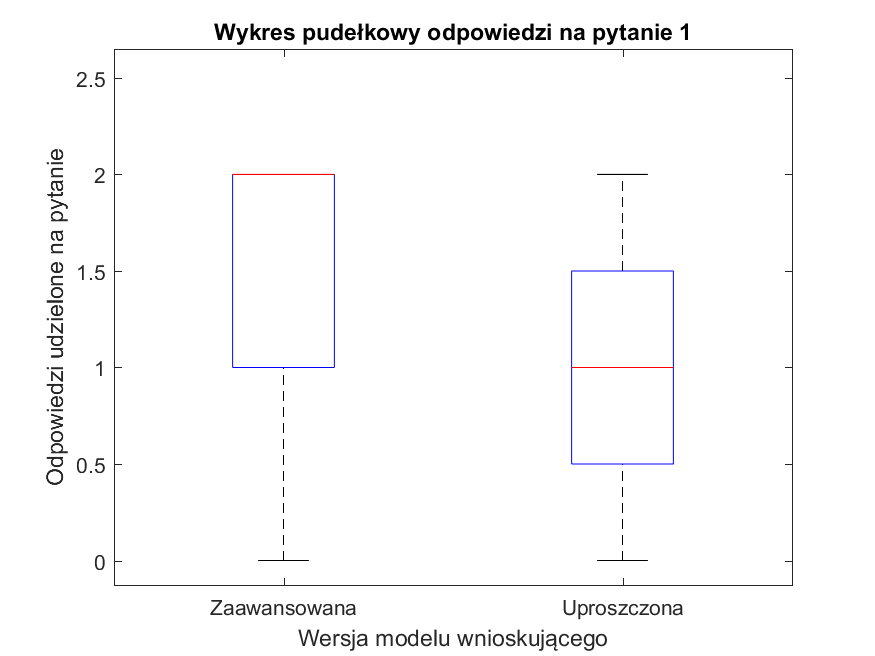
\includegraphics[scale=0.8]{rozdzial5/Ewaluacja1.png}
		\caption{Ewaluacja: pytanie 1 -- wykres pudełkowy.}
	\end{figure}
	
	\subsubsection{Obserwacje i wnioski:}
	
	Statystycznie nieco bardziej z całokształtu zadowoleni byli użytkownicy wersji zaawansowanej, stanowiącej podstawę niniejszczego badania. Całokształt ogólnego zachowania aplikacji został oceniony przez użytkowników dobrze -- z medianą 2 dla wersji zaawansowanej.


\subsection{Czy system pytał mnie o nastrój w nieodpowiednich momentach?}

	\subsubsection{Cel pytania:}
	
	Odpytywanie użytkownika musiało być najbardziej uciążliwą czynnością. Wszystkie inne działania pluginu \textit{HowAreYou} były wykonywane w tle. Celem zaawansowanej wersji było zmniejszenie tej uciążliwości.
	
	\subsubsection{Uzyskane wyniki:}
	
	\begin{table}[!h]
		\caption{Ewaluacja: pytanie 2 -- uzyskane wyniki.}
		\centering
		\begin{tabular}{|c|c|c|c|c|c|c|c|c|c|c|c|c|c|}
			\hline
			Wersja &  \multicolumn{9}{c|}{Zaawansowana} & \multicolumn{4}{c|}{Uproszczona}\\ \hline
			Identyfikator użytkownika             & 1 & 2 & 3 & 4 & 5 & 6 & 7 & 8 & 9 
			& 10 & 11 & 12 & 13 \\ \hline
			Odpowiedzi poszczególnych uczestników & -1 & -2 & 0 & 1 & -1 & -1 & 1 & 2 & 0
			& 2 & 1 & 2 & 1     \\ \hline
		\end{tabular}
	\end{table}
	
	\begin{table}[!h]
		\caption{Ewaluacja: pytanie 2 -- prosta analiza statystyczna.}
		\centering
		\begin{tabular}{|c|c|c|}
			\hline
			Wersja          & Zaawansowana & Uproszczona \\ \hline
			Wartość średnia & -0.11        & 1.50        \\ \hline
			Wariancja       &  1.61        & 0.33        \\ \hline
			Mediana         &  0.00        & 1.50        \\ \hline
		\end{tabular}
	\end{table}
	
	\begin{figure}[H]
		\centering
		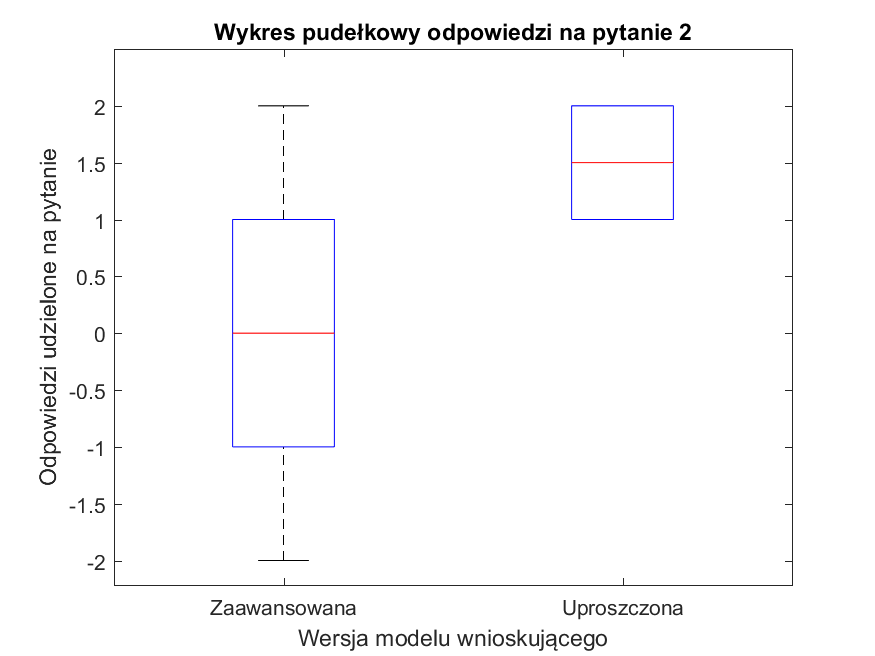
\includegraphics[scale=0.8]{rozdzial5/Ewaluacja2.png}
		\caption{Ewaluacja: pytanie 2 -- wykres pudełkowy.}
	\end{figure}
	
	\subsubsection{Obserwacje i wnioski:}
	
	Wyniki dla użytkowników podstawowej wersji aplikacji okazały się być bardzo zróżnicowane. Część badanych wskazała, że odpytywanie o nastrój im nie przeszkadzało. Pojawiły się też niestety głosy, że było to jednak irytujące. Inaczej sytuacja wygląda, jeżeli chodzi o odpowiedzi osób, wykorzystujących wersję klasyczną (z regularnym odpytywaniem) -- tutaj wszyscy użytkownicy wskazali, że byli pytani w nieodpowiednich momentach. Dzięki wykorzystaniu silnika wnioskującego i sensorów udało się więc ograniczyć w znaczący sposób uciążliwość odpytywania użytkownika.
	
	
	\subsection{Czy miałem wątpliwości jak odpowiadać na pytania o odczuwane przez siebie emocje?}
	
	\subsubsection{Cel pytania:}
	
	W tym pytaniu chodziło o sprawdzenie, jak użytkownicy odbierają wygląd i sposób działania aktywności z widokiem emotikon. Warto podkreślić, że widok emotikon został zachowany w sposób identyczny w~wersji B.
	
	\subsubsection{Uzyskane wyniki:}
	
	\begin{table}[!h]
		\caption{Ewaluacja: pytanie 3 -- uzyskane wyniki.}
		\centering
		\begin{tabular}{|c|c|c|c|c|c|c|c|c|c|c|c|c|c|}
			\hline
			Wersja &  \multicolumn{9}{c|}{Zaawansowana} & \multicolumn{4}{c|}{Uproszczona}\\ \hline
			Identyfikator użytkownika             & 1 & 2 & 3 & 4 & 5 & 6 & 7 & 8 & 9 
			& 10 & 11 & 12 & 13 \\ \hline
			Odpowiedzi poszczególnych uczestników & -2 & -1 & -1 & -1 & 0 & -2 & -1 & -2 & -1
			& -1 & 0 & -2 & -1  \\ \hline
		\end{tabular}
	\end{table}
	
	\begin{table}[!h]
		\caption{Ewaluacja: pytanie 3 -- prosta analiza statystyczna.}
		\centering
		\begin{tabular}{|c|c|c|}
			\hline
			Wersja          & Zaawansowana & Uproszczona \\ \hline
			Wartość średnia & -1.22        & -1.00       \\ \hline
			Wariancja       &  0.44        &  0.67       \\ \hline
			Mediana         & -1.00        & -1.00       \\ \hline
		\end{tabular}
	\end{table}
	\clearpage
	
	\begin{figure}[H]
		\centering
		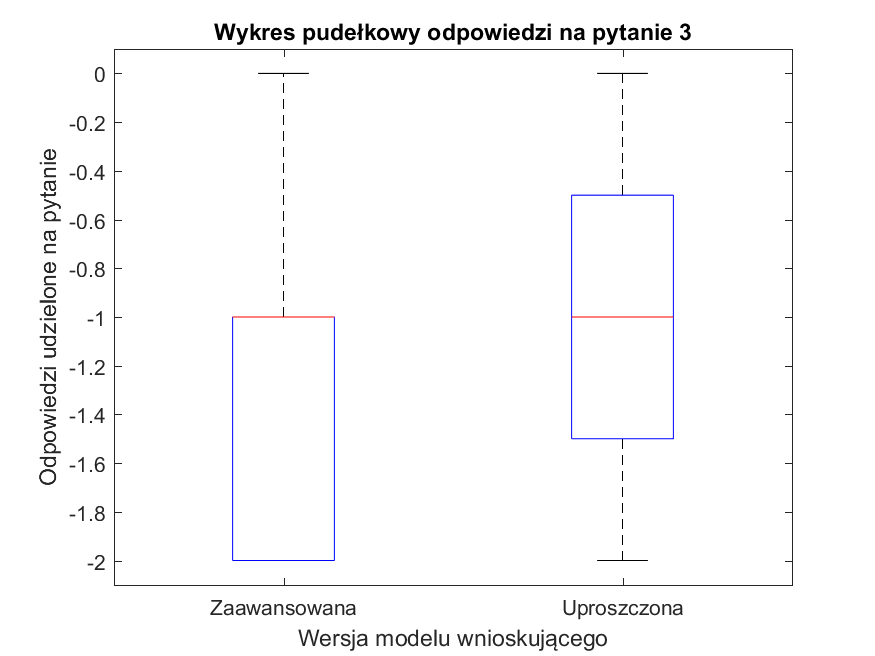
\includegraphics[scale=0.8]{rozdzial5/Ewaluacja3.png}
		\caption{Ewaluacja: pytanie 3 -- wykres pudełkowy.}
	\end{figure}
	
	\subsubsection{Obserwacje i wnioski:}
	
	Użytkownikom przypadło do gustu odpytywanie z wykorzystaniem widoku emotikon. Badani z obydwu grup wskazali w przeważającej większości, że nie mieli wątpliwości, jak odpowiadać na zadane pytania.
	
	
	\subsection{Czy miałem wątpliwości jak odpowiadać na pytania systemu o kolor odpowiadający temu, jak się czuję?}
	
	\subsubsection{Cel pytania:}
	
	W tym pytaniu chodziło o sprawdzenie, jak użytkownicy odbierają wygląd i sposób działania aktywności z widokiem mapy kolorów. Pytanie nie zostało zadane użytkownikom wersji B.
	
	\subsubsection{Uzyskane wyniki:}
	
	\begin{table}[!h]
		\caption{Ewaluacja: pytanie 4 -- uzyskane wyniki.}
		\centering
		\begin{tabular}{|c|c|c|c|c|c|c|c|c|c|c|c|c|c|}
			\hline
			Wersja &  \multicolumn{9}{c|}{Zaawansowana} & \multicolumn{4}{c|}{Uproszczona}\\ \hline
			Identyfikator użytkownika             & 1 & 2 & 3 & 4 & 5 & 6 & 7 & 8 & 9 
			& 10 & 11 & 12 & 13 \\ \hline
			Odpowiedzi poszczególnych uczestników & 2 & -2 & 1 & 1 & 2 & -2 & 1 & 2 & 0
			& --  & -- & -- & --     \\ \hline
		\end{tabular}
	\end{table}
	
	\begin{table}[!h]
		\caption{Ewaluacja: pytanie 4 -- prosta analiza statystyczna.}
		\centering
		\begin{tabular}{|c|c|c|}
			\hline
			Wersja          & Zaawansowana & Uproszczona \\ \hline
			Wartość średnia & 0.56         & --          \\ \hline
			Wariancja       & 2.53         & --          \\ \hline
			Mediana         & 1.00         & --          \\ \hline
		\end{tabular}
	\end{table}
	
	\begin{figure}[H]
		\centering
		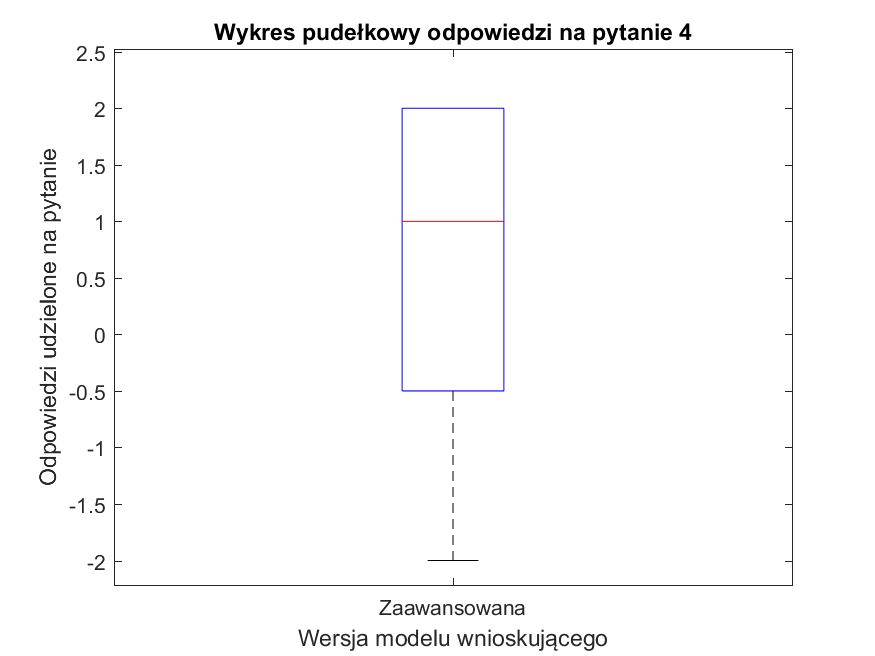
\includegraphics[scale=0.8]{rozdzial5/Ewaluacja4.png}
		\caption{Ewaluacja: pytanie 4 -- wykres pudełkowy.}
	\end{figure}
	
	\subsubsection{Obserwacje i wnioski:}
	
	Zdecydowana większość użytkowników wskazała, że miała problem przy odpowiadaniu na pytania dotyczące koloru. Może to oznaczać, że pytanie ludzi o kolor nie jest dobrym pomysłem. Istnieje ryzyko, że część spośród udzielonych odpowiedzi mogła być losowa -- spowodowana prostym kliknięciem w ekran, aby ,,pozbyć się'' uciążliwego pytania. Całkiem prawdopodobne, że potrzeba bardzo dużo danych, aby z wyników pytania o kolor wysnuć jakieś wnioski. Warto również podkreślić, że odpowiedzi znacznie różnią się miedzy sobą -- u części osób na przykład zdecydowanie wątpliwości się nie pojawiły.



\subsection{Czy określił(a) bym siebie jako umysł ścisły (inżynierski, itp.)?}

	\subsubsection{Cel pytania:}
	
	Pytanie zadano jako uzupełnienie poprzedniego. Chodziło o to, aby zdobyć chociaż namiastkę zrozumienia, jak charakter i osobowość człowieka wpływa na udzielane przez niego odpowiedzi. 
	
	\subsubsection{Uzyskane wyniki:}
	
	\begin{table}[!h]
		\caption{Ewaluacja: pytanie 5 -- uzyskane wyniki.}
		\centering
		\begin{tabular}{|c|c|c|c|c|c|c|c|c|c|c|c|c|c|}
			\hline
			Wersja &  \multicolumn{9}{c|}{Zaawansowana} & \multicolumn{4}{c|}{Uproszczona}\\ \hline
			Identyfikator użytkownika             & 1 & 2 & 3 & 4 & 5 & 6 & 7 & 8 & 9 
			& 10 & 11 & 12 & 13 \\ \hline
			Odpowiedzi poszczególnych uczestników & 1 & -2 & 2 & 2 & 0 & -2 & 2 & 2 & -1
			& --  & -- & -- & --    \\ \hline
			Odpowiedzi na poprzednie pytanie      & 2 & -2 & 1 & 1 & 2 & -2 & 1 & 2 & 0
			& --  & -- & -- & --    \\ \hline
		\end{tabular}
	\end{table}
	
	\begin{table}[!h]
		\caption{Ewaluacja: pytanie 5 -- prosta analiza statystyczna.}
		\centering
		\begin{tabular}{|c|c|c|}
			\hline
			Wersja          & Zaawansowana & Uproszczona \\ \hline
			Wartość średnia & 0.44         & --          \\ \hline
			Wariancja       & 3.03         & --          \\ \hline
			Mediana         & 1.00         & --          \\ \hline
		\end{tabular}
	\end{table}
	
	\begin{figure}[H]
		\centering
		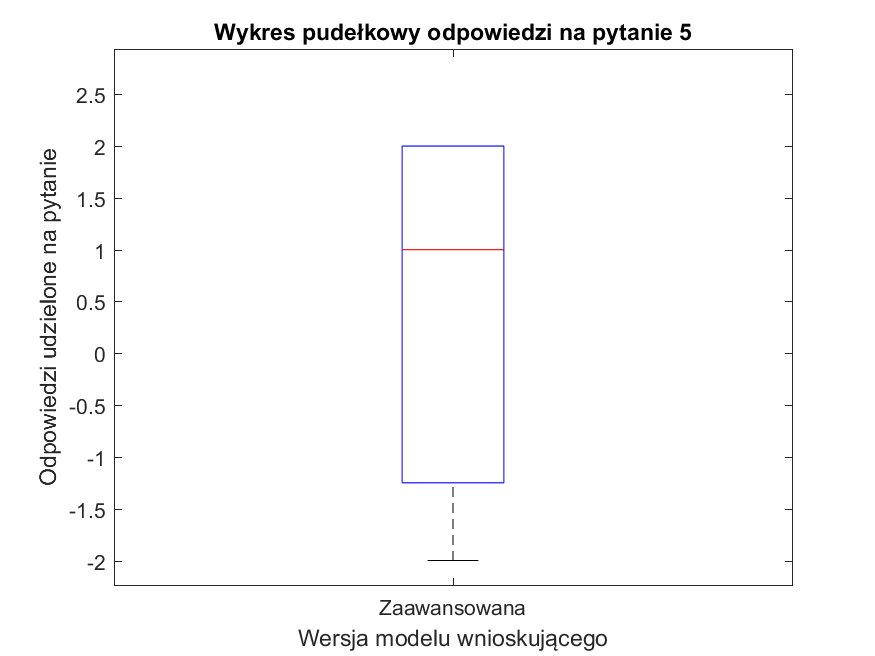
\includegraphics[scale=0.8]{rozdzial5/Ewaluacja5.png}
		\caption{Ewaluacja: pytanie 5 -- wykres pudełkowy.}
	\end{figure}
	
	\subsubsection{Obserwacje i wnioski:}
	
	Większość uczestników testu to inżynierowie. Prawdopodobnie naturalnie więc określili oni siebie jako umysły ścisłe. W teście wzięły też udział osoby o innych zainteresowaniach -- na przykład absolwentka ASP czy studentka medycyny. Pojawiły się więc również odpowiedzi negatywne. Co kluczowe przy tym pytaniu, tak jak przypuszczano, pomimo małej próbki można dostrzec nieznaczną korelację -- osobom określającym siebie jako umysł ścisły większą trudność sprawiło odpowiadanie na pytania dotyczące kolorów. Dobrym pomysłem, było więc pozwolenie użytkownikom pluginu na wybór sposobu, w jaki chcą odpowiadać na pytania dotyczące emocji -- czy to z wykorzystaniem widoku emotikon, czy to za pomocą mapy kolorów, czy poprzez rozpoznawanie emocji na podstawie fotografii. Domyślnie wszystkie opcje są aktywne. Można wybrać również zero, jedną, czy dwie z nich.
	
	
\subsection{Czy system NIE przeszkadzał mi w korzystaniu z telefonu?}
	
	\subsubsection{Cel pytania:}
	
	Jednym z celów rozszerzenia \textit{HowAreYou} było zmniejszenie uciążliwości odpytywania użytkownika, między innymi przez stworzenie prostego, intuicyjnego i jak najbardziej nieinwazyjnego interfejsu. Pytanie weryfikuje tę funkcjonalność.
	
	W podobnych ankietach ludzie często pomijają słowo nie, dlatego zostało ono dodatkowo wyróżnione.
	
	\subsubsection{Uzyskane wyniki:}
	
	\begin{table}[!h]
		\caption{Ewaluacja: pytanie 6 -- uzyskane wyniki.}
		\centering
		\begin{tabular}{|c|c|c|c|c|c|c|c|c|c|c|c|c|c|}
			\hline
			Wersja &  \multicolumn{9}{c|}{Zaawansowana} & \multicolumn{4}{c|}{Uproszczona}\\ \hline
			Identyfikator użytkownika             & 1 & 2 & 3 & 4 & 5 & 6 & 7 & 8 & 9 
			& 10 & 11 & 12 & 13 \\ \hline
			Odpowiedzi poszczególnych uczestników & -1 & -2 & -2 & 1 & 0 & 1 & 2 & -1 & 1
			& -2 & 1 & -1 & 0     \\ \hline
		\end{tabular}
	\end{table}
	
	\begin{table}[!h]
		\caption{Ewaluacja: pytanie 6 -- prosta analiza statystyczna.}
		\centering
		\begin{tabular}{|c|c|c|}
			\hline
			Wersja          & Zaawansowana & Uproszczona \\ \hline
			Wartość średnia & -0.11        & -0.50       \\ \hline
			Wariancja       &  2.11        &  1.67       \\ \hline
			Mediana         &  0.00        & -0.50       \\ \hline
		\end{tabular}
	\end{table}
	\clearpage
	
	\begin{figure}[H]
		\centering
		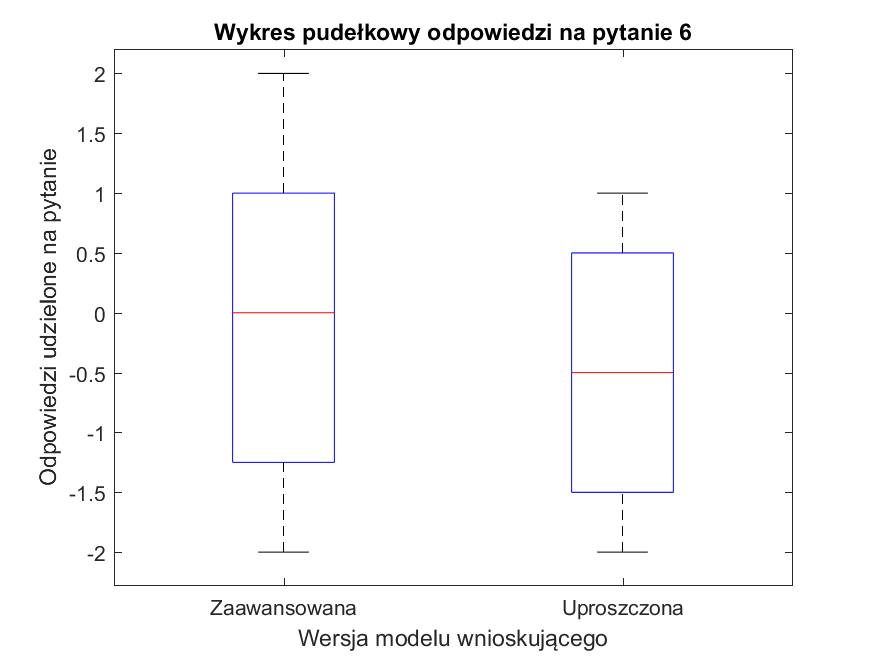
\includegraphics[scale=0.8]{rozdzial5/Ewaluacja6.png}
		\caption{Ewaluacja: pytanie 6 -- wykres pudełkowy.}
	\end{figure}
	
	\subsubsection{Obserwacje i wnioski:}
	
	Zarówno niniejsze pytanie, jak i to o nieodpowiednich momentach, wskazują, że system owszem był delikatnie uciążliwy, bo każde przerywanie i zadawanie pytań jest uciążliwe. Z drugiej jednak strony generalnie oceny użytkowników są raczej wysokie, więc plugin w wersji zaawansowanej został przygotowany jako przyjazny dla użytkowników. Należy też odnotować, że system okazał się bardziej uciążliwy dla użytkowników wersji prostej.
	
	
	
\subsection{Czy system NIE zabierał mi zbyt dużo czasu?}
	
	\subsubsection{Cel pytania:}
	
	Jednym z celów rozszerzenia \textit{HowAreYou} było zmniejszenie uciążliwości odpytywania użytkownika, między innymi przez stworzenie prostego, intuicyjnego i jak najbardziej nieinwazyjnego interfejsu. Pytanie weryfikuje tę funkcjonalność.
	
	W podobnych ankietach często ludzie pomijają słowo nie, dlatego zostało ono dodatkowo wyróżnione.
	
	\subsubsection{Uzyskane wyniki:}
	
	\begin{table}[!h]
		\caption{Ewaluacja: pytanie 7 -- uzyskane wyniki.}
		\centering
		\begin{tabular}{|c|c|c|c|c|c|c|c|c|c|c|c|c|c|}
			\hline
			Wersja &  \multicolumn{9}{c|}{Zaawansowana} & \multicolumn{4}{c|}{Uproszczona}\\ \hline
			Identyfikator użytkownika             & 1 & 2 & 3 & 4 & 5 & 6 & 7 & 8 & 9 
			& 10 & 11 & 12 & 13 \\ \hline
			Odpowiedzi poszczególnych uczestników & -2 & -1 & -1 & 0 & 1 & -1 & 1 & 0 & -1
			& -1 & 0 & 1 & -2     \\ \hline
		\end{tabular}
	\end{table}
	
	\begin{table}[!h]
		\caption{Ewaluacja: pytanie 7 -- prosta analiza statystyczna.}
		\centering
		\begin{tabular}{|c|c|c|}
			\hline
			Wersja          & Zaawansowana & Uproszczona \\ \hline
			Wartość średnia & -0.44        & -0.50       \\ \hline
			Wariancja       &  1.03        &  1.67       \\ \hline
			Mediana         & -1.00        & -0.50       \\ \hline
		\end{tabular}
	\end{table}
	
	\begin{figure}[H]
		\centering
		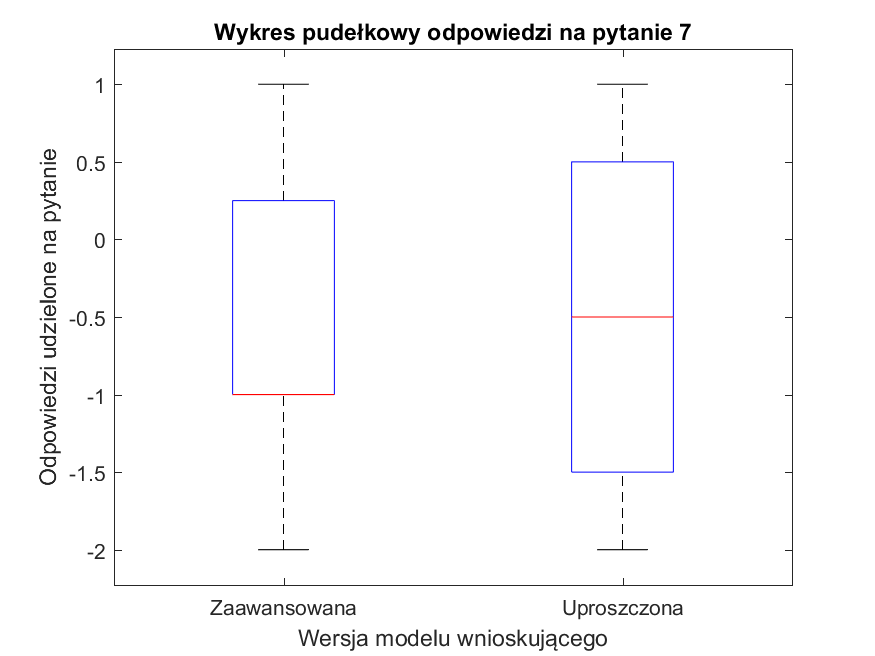
\includegraphics[scale=0.8]{rozdzial5/Ewaluacja7.png}
		\caption{Ewaluacja: pytanie 7 -- wykres pudełkowy.}
	\end{figure}
	
	\subsubsection{Obserwacje i wnioski:}
	
	Pomimo tego, że w jednym z poprzednich pytań spora część użytkowników wskazała, że była pytana w nieodpowiednich momentach, czy też że system przeszkadzał im w korzystaniu z telefonu, w tej kwestii użytkownicy byli raczej zgodni -- w większości określili system jako nieczasochłonny.
	
	
	
\subsection{Czy skanowanie nastroju z wykorzystaniem kamery telefonu było dla mnie zauważalne?}
	
	\subsubsection{Cel pytania:}
	
	Celem analizowania nastroju poprzez wykonywanie fotografii było ograniczenie uciążliwości działania systemu poprzez przeniesienie części odpowiedzialności z jawnego odpytywania na niejawne skanowanie. W teorii -- skanowanie nie powinno być zauważalne dla użytkownika. Pytanie dodano, aby tę hipotezę potwierdzić. Zadano je tylko tym uczestnikom badania, którzy wykorzystywali funkcjonalność kamery w wersji rozszerzonej.
	
	\subsubsection{Uzyskane wyniki:}
	
	\begin{table}[!h]
		\caption{Ewaluacja: pytanie 8 -- uzyskane wyniki.}
		\centering
		\begin{tabular}{|c|c|c|c|c|c|c|c|c|c|c|c|c|c|}
			\hline
			Wersja &  \multicolumn{9}{c|}{Zaawansowana} & \multicolumn{4}{c|}{Uproszczona}\\ \hline
			Identyfikator użytkownika             & 1 & 2 & 3 & 4 & 5 & 6 & 7 & 8 & 9 
			& 10 & 11 & 12 & 13 \\ \hline
			Odpowiedzi poszczególnych uczestników & -1 & -2 & 0 & 0 & -1 & -2 & -1 & 1 & -1
			& --  & -- & -- & -- \\ \hline
		\end{tabular}
	\end{table}
	
	\begin{table}[!h]
		\caption{Ewaluacja: pytanie 8 -- prosta analiza statystyczna.}
		\centering
		\begin{tabular}{|c|c|c|}
			\hline
			Wersja          & Zaawansowana & Uproszczona \\ \hline
			Wartość średnia & -0.78        & --          \\ \hline
			Wariancja       &  0.94        & --          \\ \hline
			Mediana         & -1.00        & --          \\ \hline
		\end{tabular}
	\end{table}
	\clearpage
	
	\begin{figure}[H]
		\centering
		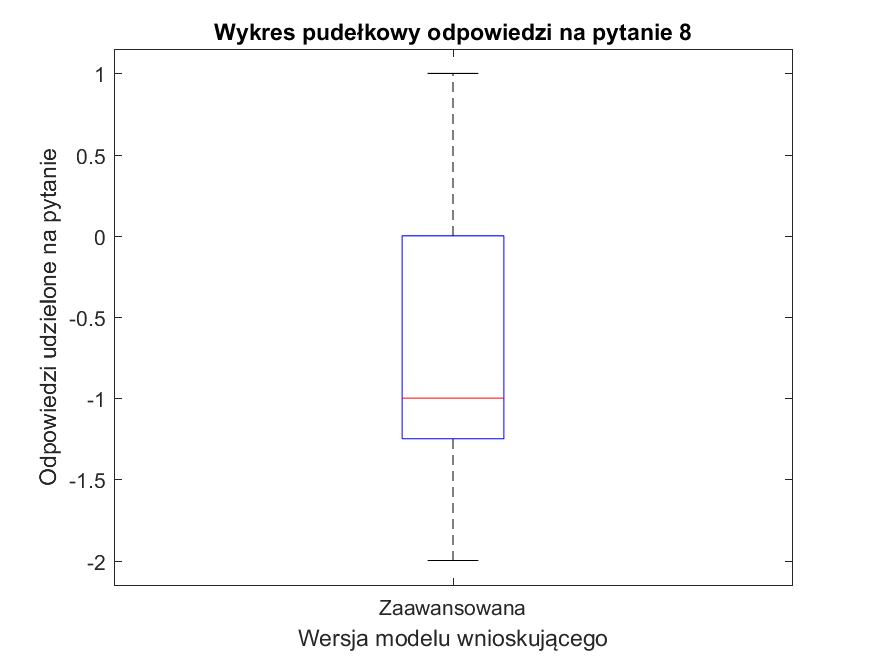
\includegraphics[scale=0.8]{rozdzial5/Ewaluacja8.png}
		\caption{Ewaluacja: pytanie 8 -- wykres pudełkowy.}
	\end{figure}
	
	\subsubsection{Uzyskane wyniki -- wersja uproszczona:}
	
	Nie dotyczy.
	
	\subsubsection{Obserwacje i wnioski:}
	
	Większość użytkowników wskazała, że podczas kilkudniowego badania wykorzystywanie kamery telefonu nie było dla nich zauważalne. 
	
	
	
\subsection{Czy skanowanie nastroju z wykorzystaniem kamery telefonu wpływało na moje codzienne zachowanie? Czy mogłoby być na dłuższą metę uciążliwe?}
	
	\subsubsection{Cel pytania:}
	
	Celem pytania było zbadanie, jak świadomość bycia fotografowanym wpływa na uczestnika badania. Chodziło także o zestawienie tego pytania z poprzednim -- o zauważalność skanowania.
	
	\subsubsection{Uzyskane wyniki:}
	
	\begin{table}[!h]
		\caption{Ewaluacja: pytanie 9 -- uzyskane wyniki.}
		\centering
		\begin{tabular}{|c|c|c|c|c|c|c|c|c|c|c|c|c|c|}
			\hline
			Wersja &  \multicolumn{9}{c|}{Zaawansowana} & \multicolumn{4}{c|}{Uproszczona}\\ \hline
			Identyfikator użytkownika             & 1 & 2 & 3 & 4 & 5 & 6 & 7 & 8 & 9 
			& 10 & 11 & 12 & 13 \\ \hline
			Odpowiedzi poszczególnych uczestników & 1 & 2 & 1 & 1 & 0 & 1 & -1 & -1 & 1
			& -- & -- & -- & --     \\ \hline
		\end{tabular}
	\end{table}
	
	\begin{table}[!h]
		\caption{Ewaluacja: pytanie 9 -- prosta analiza statystyczna.}
		\centering
		\begin{tabular}{|c|c|c|}
			\hline
			Wersja          & Zaawansowana & Uproszczona \\ \hline
			Wartość średnia & 0.56         & --          \\ \hline
			Wariancja       & 1.03         & --          \\ \hline
			Mediana         & 1.00         & --          \\ \hline
		\end{tabular}
	\end{table}
	
	\begin{figure}[H]
		\centering
		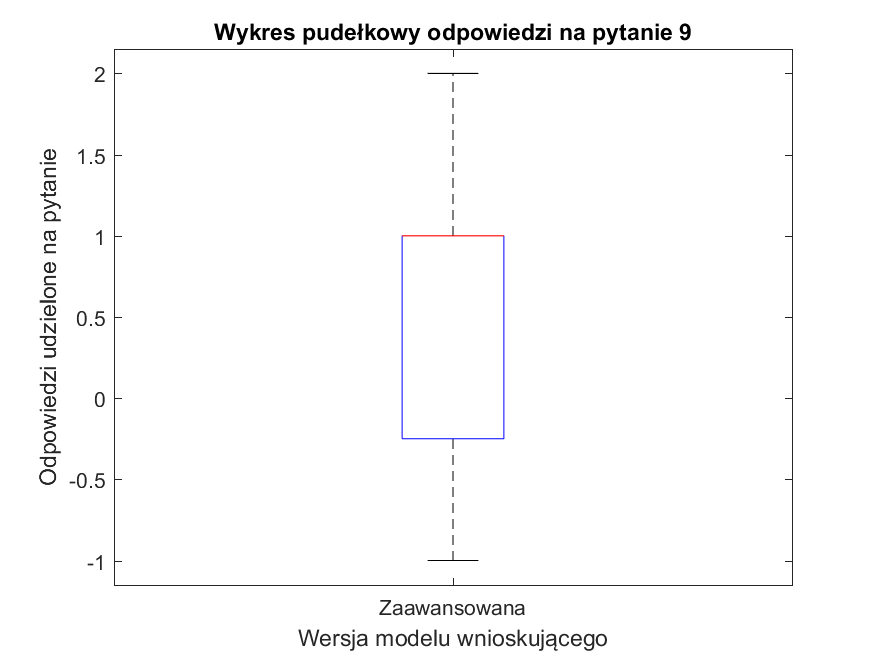
\includegraphics[scale=0.8]{rozdzial5/Ewaluacja9.png}
		\caption{Ewaluacja: pytanie 9 -- wykres pudełkowy.}
	\end{figure}
	
	\subsubsection{Obserwacje i wnioski:}
	
	Pomimo, że w poprzednim pytaniu większość uczestników wskazała, że przy kilkudniowym badaniu samo skanowanie nastroju nie było dla nich zauważalne, to jednak miało ono wpływ na ich codzienne zachowanie. To naturalne -- każdy człowiek chroni swoją prywatność. Taka świadomość bycia podglądanym wymusza na nas pewne zmiany.
	
	
\subsection{Czy system działał zgodnie z konfiguracją i z moimi oczekiwaniami?}
	
	\subsubsection{Cel pytania:}
	
	Celem pytania było sprawdzenie oceny działania systemu przez użytkowników, abstrahując od kwestii wygody czy uciążliwości. Chodziło o sprawdzenie niezawodności i ewentualnie możliwości konfiguracji systemu.
	
	\subsubsection{Uzyskane wyniki:}
	
	\begin{table}[!h]
		\caption{Ewaluacja: pytanie 10 -- uzyskane wyniki.}
		\centering
		\begin{tabular}{|c|c|c|c|c|c|c|c|c|c|c|c|c|c|}
			\hline
			Wersja &  \multicolumn{9}{c|}{Zaawansowana} & \multicolumn{4}{c|}{Uproszczona}\\ \hline
			Identyfikator użytkownika             & 1 & 2 & 3 & 4 & 5 & 6 & 7 & 8 & 9 
			& 10 & 11 & 12 & 13 \\ \hline
			Odpowiedzi poszczególnych uczestników & 1 & 2 & 1 & 0 & 1 & 2 & 1 & 1 & 2
			& -1 & 1 & 0 & 1    \\ \hline
		\end{tabular}
	\end{table}
	
	\begin{table}[!h]
		\caption{Ewaluacja: pytanie 10 -- prosta analiza statystyczna.}
		\centering
		\begin{tabular}{|c|c|c|}
			\hline
			Wersja          & Zaawansowana & 0.25        \\ \hline
			Wariancja       & 0.44         & 0.92        \\ \hline
			Mediana         & 1.00         & 0.50        \\ \hline
		\end{tabular}
	\end{table}
	
	\begin{figure}[H]
		\centering
		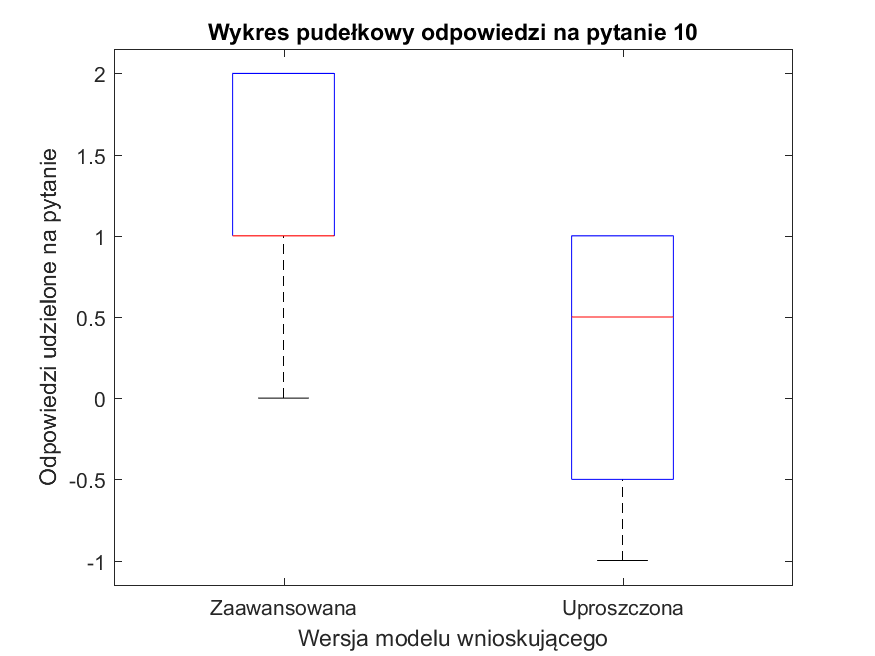
\includegraphics[scale=0.8]{rozdzial5/Ewaluacja10.png}
		\caption{Ewaluacja: pytanie 10 -- wykres pudełkowy.}
	\end{figure}
	
	\subsubsection{Obserwacje i wnioski:}
	
	Działanie pluginu \textit{HowAreYou} zostało przez użytkowników ocenione dobrze. System zebrał same oceny pozytywne i neuralne dla wersji rozszerzonej i tylko jedną negatywną dla prostego odpytywania z~wykorzystaniem widoku emotikon.
	
	
	\chapter{Podsumowanie}
\label{cha:podsumowanie}


%---------------------------------------------------------------------------

\section{Podsumowanie i wnioski}
\label{sec:podsumowanieIWnioski}

Celem pracy było zaprojektowanie, implementacja i ewaluacja mechanizmu pozyskiwania wiedzy o  stanie emocjonalnym użytkownika w systemach \textit{affective computing}.  

Na potrzeby pracy zaprojektowana i zaimplementowana została aplikacja mobilna pozwalająca na uczynienie jawnej mediacji wiedzy możliwie nieintruzywną (poprzez wnioskowanie oparte na monitorowaniu czynników zewnętrznych) oraz na przeprowadzenie niejawnej mediacji (z wykorzystaniem aparatu fotograficznego telefonu). 

Cel udało się zrealizować, a potwierdzeniem tego są wyniki ewaluacji z poprzedniego rozdziału. Badanie wśród grona użytkowników potwierdziło, że stworzona aplikacja spełniła swoje podstawowe założenia, przede wszystkim czyniąc proces mediacji wiedzy bardziej skutecznym i przyjaznym dla uczestnika badania.

Podczas realizacji pracy wyprowadzono następujące wnioski:

\begin{itemize}
	\item Odczytywanie emocji przez urządzenia może przyczynić się do polepszenia jakości życia w kategoriach: rozrywki, nauki, pracy, marketingu, bezpieczeństwa i wielu innych.
	
	\item Smartfon, jako urządzenie, które zawsze jest pod ręką, nadaje się bardzo dobrze do monitorowania nastroju użytkownika.
	
	\item Na dłuższą metę nagrywanie dźwięku, robienie zdjęć, czy odpytywanie użytkownika nie ma racji bytu z uwagi na naturalną dla człowieka potrzebę chronienia swojej prywatności. Konieczne jest wprowadzenie nowych metod rozpoznawania nastroju, najlepiej przez wykorzystanie istniejących sposobów akwizycji danych.
	
	\item Dane z~dotychczas zrozumiałych i niezrozumiałych dla maszyny źródeł są częściowo skorelowane. Przez czasową akwizycję informacji z~jednej i drugiej kategorii u wielu ludzi można stworzyć bazę, dzięki której w przyszłości rozpoznawanie nastroju nie będzie dla użytkownika w żaden sposób uciążliwe.
	
	\item Konieczna jest aplikacja do gromadzenia danych. Musi być bezpieczna, lekka, nieuciążliwa, prosta i intuicyjna. Musi dawać użytkownikowi kontrolę nad treściami i przesyłać zgromadzone informacje do bazy dostępnej na serwerze.
	
	\item Framework \textit{AWARE} pozwala deweloperom na skuteczną implementację: inteligentnego mechanizmu odpytywania użytkownika, mechanizmu automatycznej obsługi kamery bez ingerencji użytkownika, transferu danych w kierunku serwera czy odpowiedniego reagowania na zdarzenia takie jak odblokowanie ekranu, wykonanie zdjęcia, wybór przycisku powiadomienia, zmiana opcji.
\end{itemize}


%---------------------------------------------------------------------------

\section{Możliwości dalszego rozwoju}
\label{sec:mozwliwosciDalszegoRozwoju}

Przygotowana na potrzeby tej pracy aplikacja mobilna \textit{HowAreYou} spełniła założone cele, jakimi były uczynienie jawnej mediacji wiedzy możliwie nieintruzywną (poprzez wnioskowanie oparte na monitorowaniu czynników zewnętrznych) oraz na przeprowadzenie niejawnej mediacji (z wykorzystaniem aparatu fotograficznego telefonu), co potwierdziła ewaluacja. Realizacja pracy pozwoliła na wyliczenie szeregu kolejnych możliwości, które można zastosować rozbudowując istniejące rozwiązanie w celu jeszcze większego usprawnienia mediacji wiedzy:

\begin{itemize}
	\item Możliwości aplikacji możemy w łatwy sposób zwiększyć rozbudowując model HMR. W tym celu należałoby zwiększyć liczbę czynników, które można wykorzystać w tabelach w modelu wnioskującym (tzw. \textit{callbacks}). Implementacja dodatkowych wywołań opartych na sensorach, informacjach udostępnianych przez system Android czy nawet dodatkowych elementach oprogramowania (takich jak np. specjalistyczna klawiatura software'owa pozwalacjąca gromadzić kolejne dane) może pozwolić na tworzenie bardziej zaawansowanych i bardziej skutecznych modeli.
	
	\item Implementacja dodatkowych obserwatorów (ang. \textit{observers}) może pozwolić na częstsze wnioskowanie, a co za tym idzie na bardziej dynamiczne, szybsze, skuteczniejsze reagowanie na zmieniające się zewnętrzne warunki.
	
	\item Inną z~możliwości jest wprowadzenie kolejnej funkcjonalności pozwalającej gromadzić informaje czy użytkownik jest zadowolony ze skuteczności odpytywania (jaką daje na przykład przesunięcie w bok, czyli opcja \textit{Nie teraz} w widoku emocji czy widoku koloru -- taki wybór będzie sygnałem dla pluginu, że w tej sytuacji nie należy przeszkadzać użytkownikowi). Łącząc te dane z danymi już zgromadzonymi w bazie \textit{SQLite}, można stworzyć model samodzielnie odkrywający zależności i ostatecznie w ten sposób dynamicznie wykształcać reguły, które obecnie muszą być zapisane w formacie \textit{XTT2} w modelu HMR.
	
	\item Ostatnią z~zaproponowanych w niniejszej pracy możliwości dalszego rozwoju pluginu \textit{HowAreYou} jest rozbudowanie systemu odpytywania użytkownika o emocje. Jedną z~opcji jest tutaj integracja już istniejącej aplikacji, która realizuje taki dialog z~użytkownikiem. 
	
	Przykładem może być tutaj rozwiązanie zrealizowane w ramach pracy \cite{ArkadiuszLis}, czyli analiza możliwości przeniesienia i uruchomienia na platformie Android istniejących środowisk do przeprowadzania eksperymentów, a następnie	opracowany został zbiór \textit{widgetów} służących do zbierania subiektywnych afektywnych ocen użytkowników w eksperymentach z~użyciem urządzeń mobilnych.
	
	Poniższe grafiki przedstawiają przykładowe \textit{widgety} z~powyższej pracy, które zostały dołączone do pluginu \textit{HowAreYou} z~wykorzystaniem widoku \textit{WebView}. Są to:
	
	\begin{itemize}
		\item \textit{Geneva Emotion Wheel} -- ,,Metoda opracowana przez profesora Klausa Scherera składa się z~dyskretnych grup emocji ułożonych w formie koła'' \cite{ArkadiuszLis}.
		
		\item Koło Plutchika -- \textit{widget} oparty o postać koła w formie ,,róży wiatrów'' \cite{ArkadiuszLis}.
	\end{itemize}
	
	\begin{figure}[H]
		\centering
		\begin{subfigure}{0.35\textwidth}
			\centering
			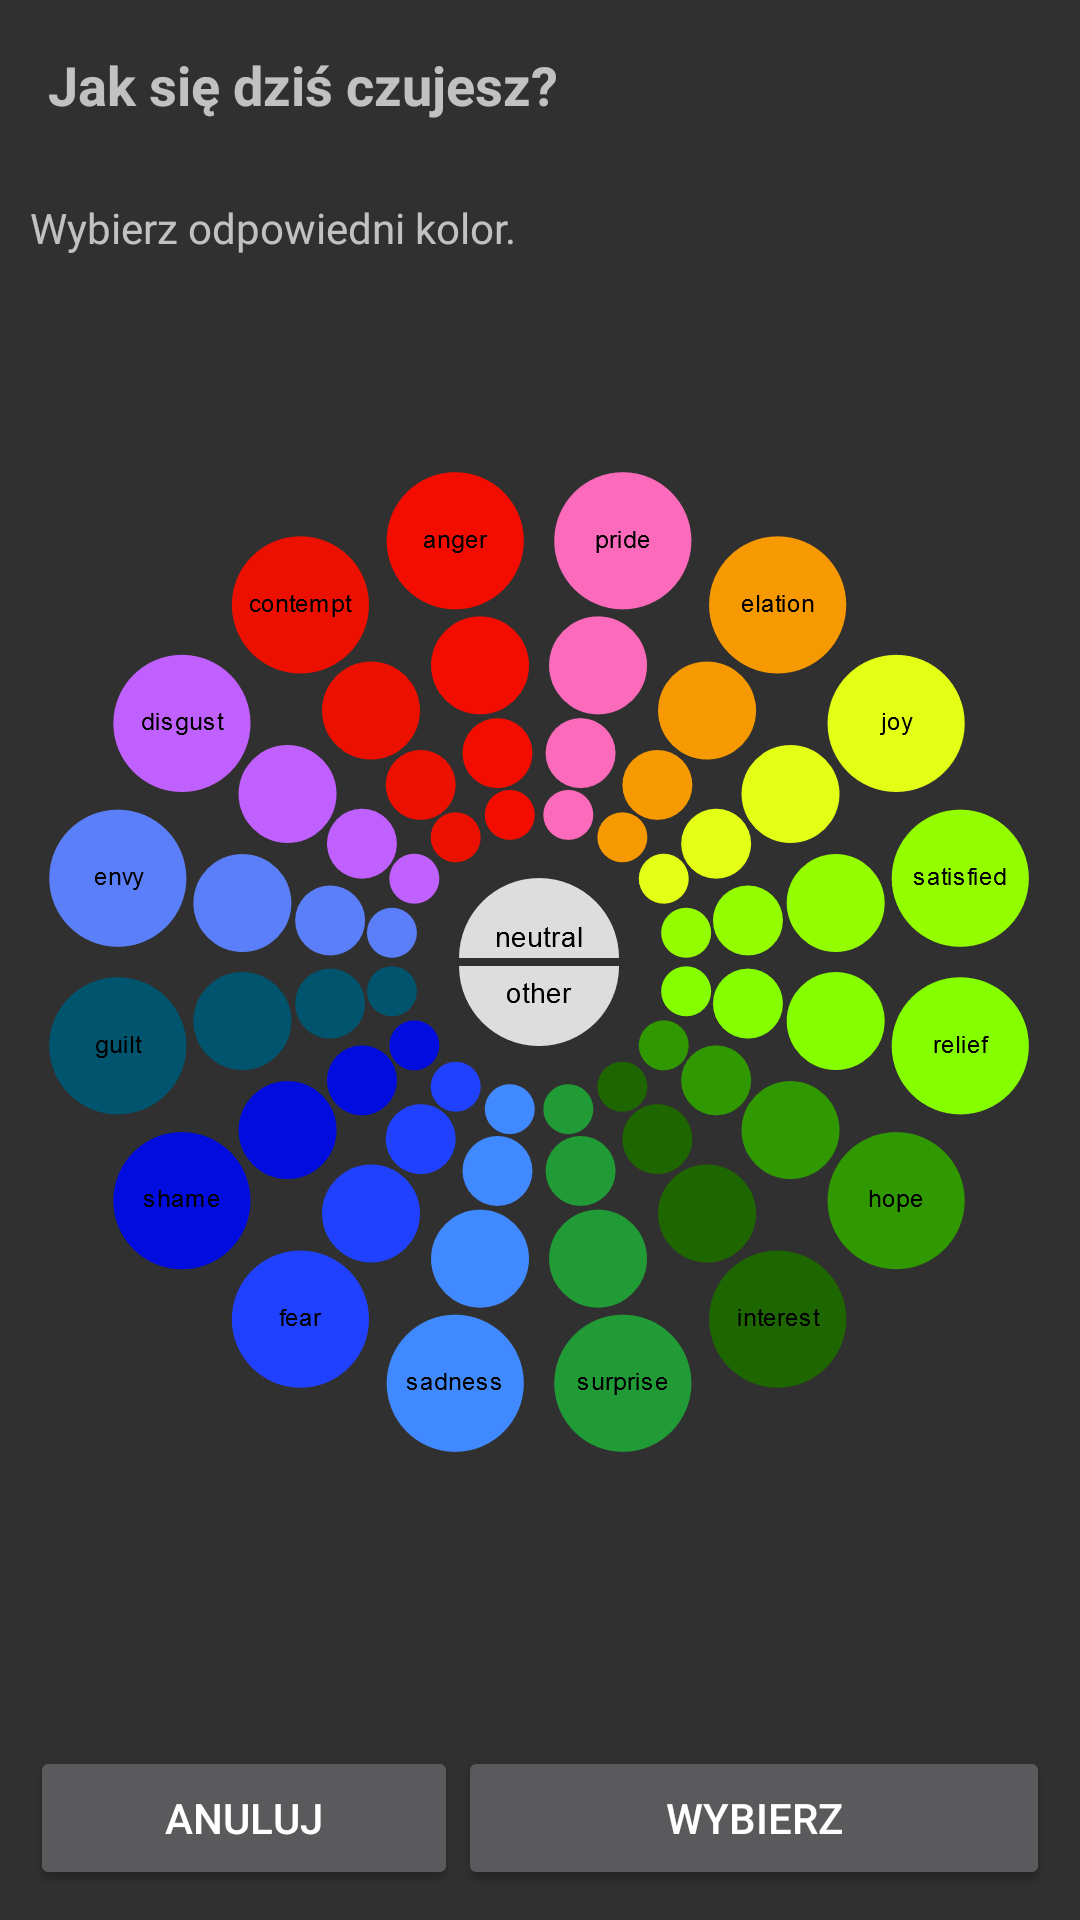
\includegraphics[scale=0.22]{rozdzial6/jspsych-geneva-wheel.png}
			\subcaption{\label{subfigure_a}}
		\end{subfigure}
		\begin{subfigure}{0.35\textwidth}
			\centering
			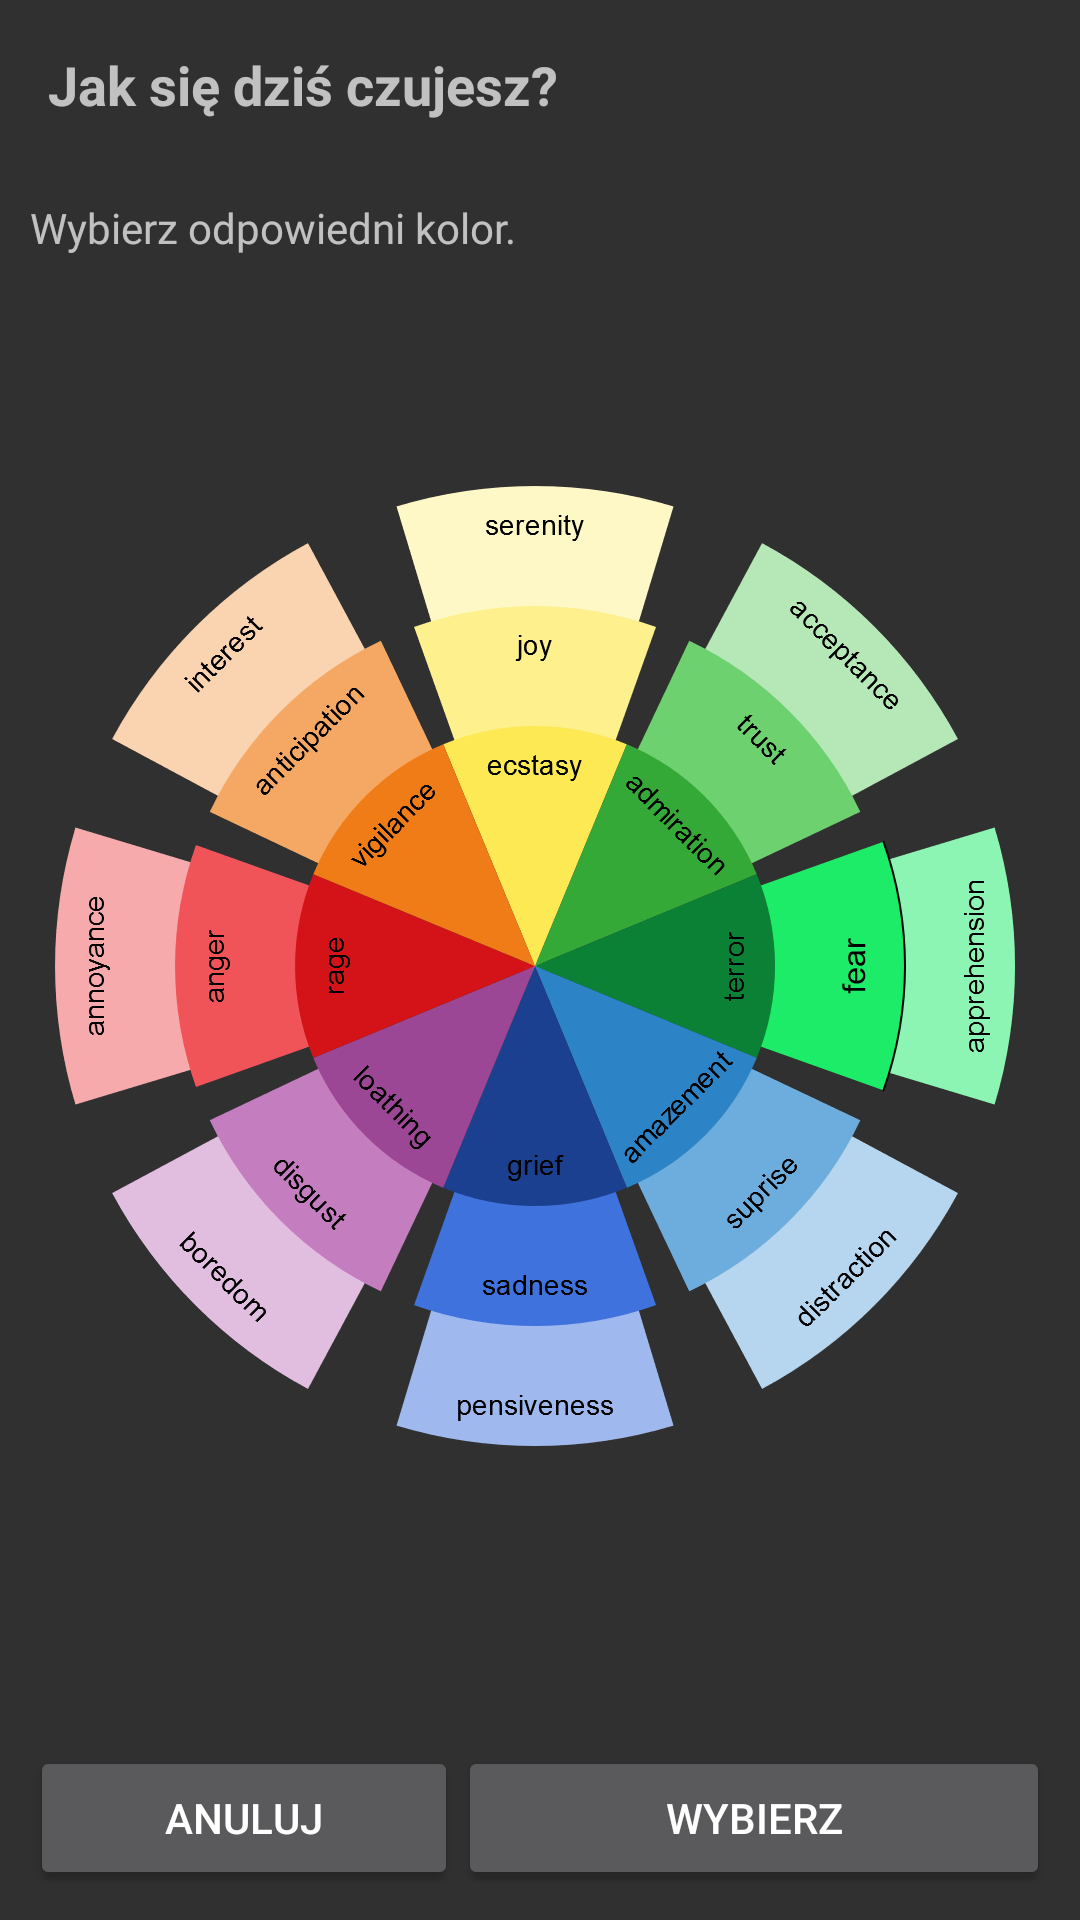
\includegraphics[scale=0.22]{rozdzial6/jspsych-plutchik-wheel-2}
			\subcaption{\label{subfigure_b}}
		\end{subfigure}
		\caption{ Zaawansowane \textit{widgety} zintegrowane z~pluginem \textit{HowAreYou: } \textit{Geneva Emotion Wheel} (a) oraz Koło Plutchika (b).}
	\end{figure}
	
\end{itemize}
	
	\appendix
	\chapter{Instalacja i pierwsze uruchomienie -- instrukcja krok po kroku}
\label{cha:instalacjaIPierwszeUruchomienie}

Klient \textit{AWARE} jest aplikacją w~fazie intensywnego rozwoju. W ostatnim czasie twórcom niemal udało się dostosować go do najnowszych wymagań firmy Google dla najnowszej wersji systemu Android Pie i umieścić wersję beta w~Sklepie Play. Jedym z~warunków była rezygnacja ze wsparcia pluginów tworzonych przez niezależnych deweloperów i integracja wewnątrz aplikacji klienckiej oficjalnie dostępnych pluginów\cite{AwareFramework}.

W związku z~powyższym, aplikacja \textit{HowAreYou} nie zostanie zainstalowana w~klasyczny sposób. Zamiast sklepu Play do instalacji zostanie wykorzystana przeglądarka. Użytkownik musi przejść poprzez 3 etapy, które pozwolą na poprawną instalację, konfigurację i uruchomienie aplikacji klienta oraz pluginu \textit{HowAreYou}. Niniejsza instrukcja wraz z~graficznymi ilustracjami krok po kroku prowadzi przez ten proces, który na pierwszy rzut oka może wydawać się skomplikowany.

%---------------------------------------------------------------------------

\section{Etap 1: Zezwolenie na instalację dodatkowych pakietów}
\label{sec:zezwolenieNaInstalacjeDodatkowychPakietow}

W pierwszej kolejności pozwolimy przeglądarce na instalację dodatkowych pakietów.

\begin{enumerate}
	
	\item Przejdź do \textit{Ustawień} systemu Android.
	
	\item Wybierz \textit{Aplikacje i powiadomienia}, a następnie \textit{Zaawansowane}.
	
	\item Wybierz \textit{Specjalny dostęp do aplikacji}, a następnie \textit{Instalowanie nieznanych aplikacji}.
	
	\item Znajdź przeglądarkę, którą na co dzień używasz.
	
	\item Kliknij \textit{Zezwól z~tego źródła}.
	\clearpage
	
	\begin{figure}[H]
		\centering
		\begin{subfigure}{0.35\textwidth}
			\centering
			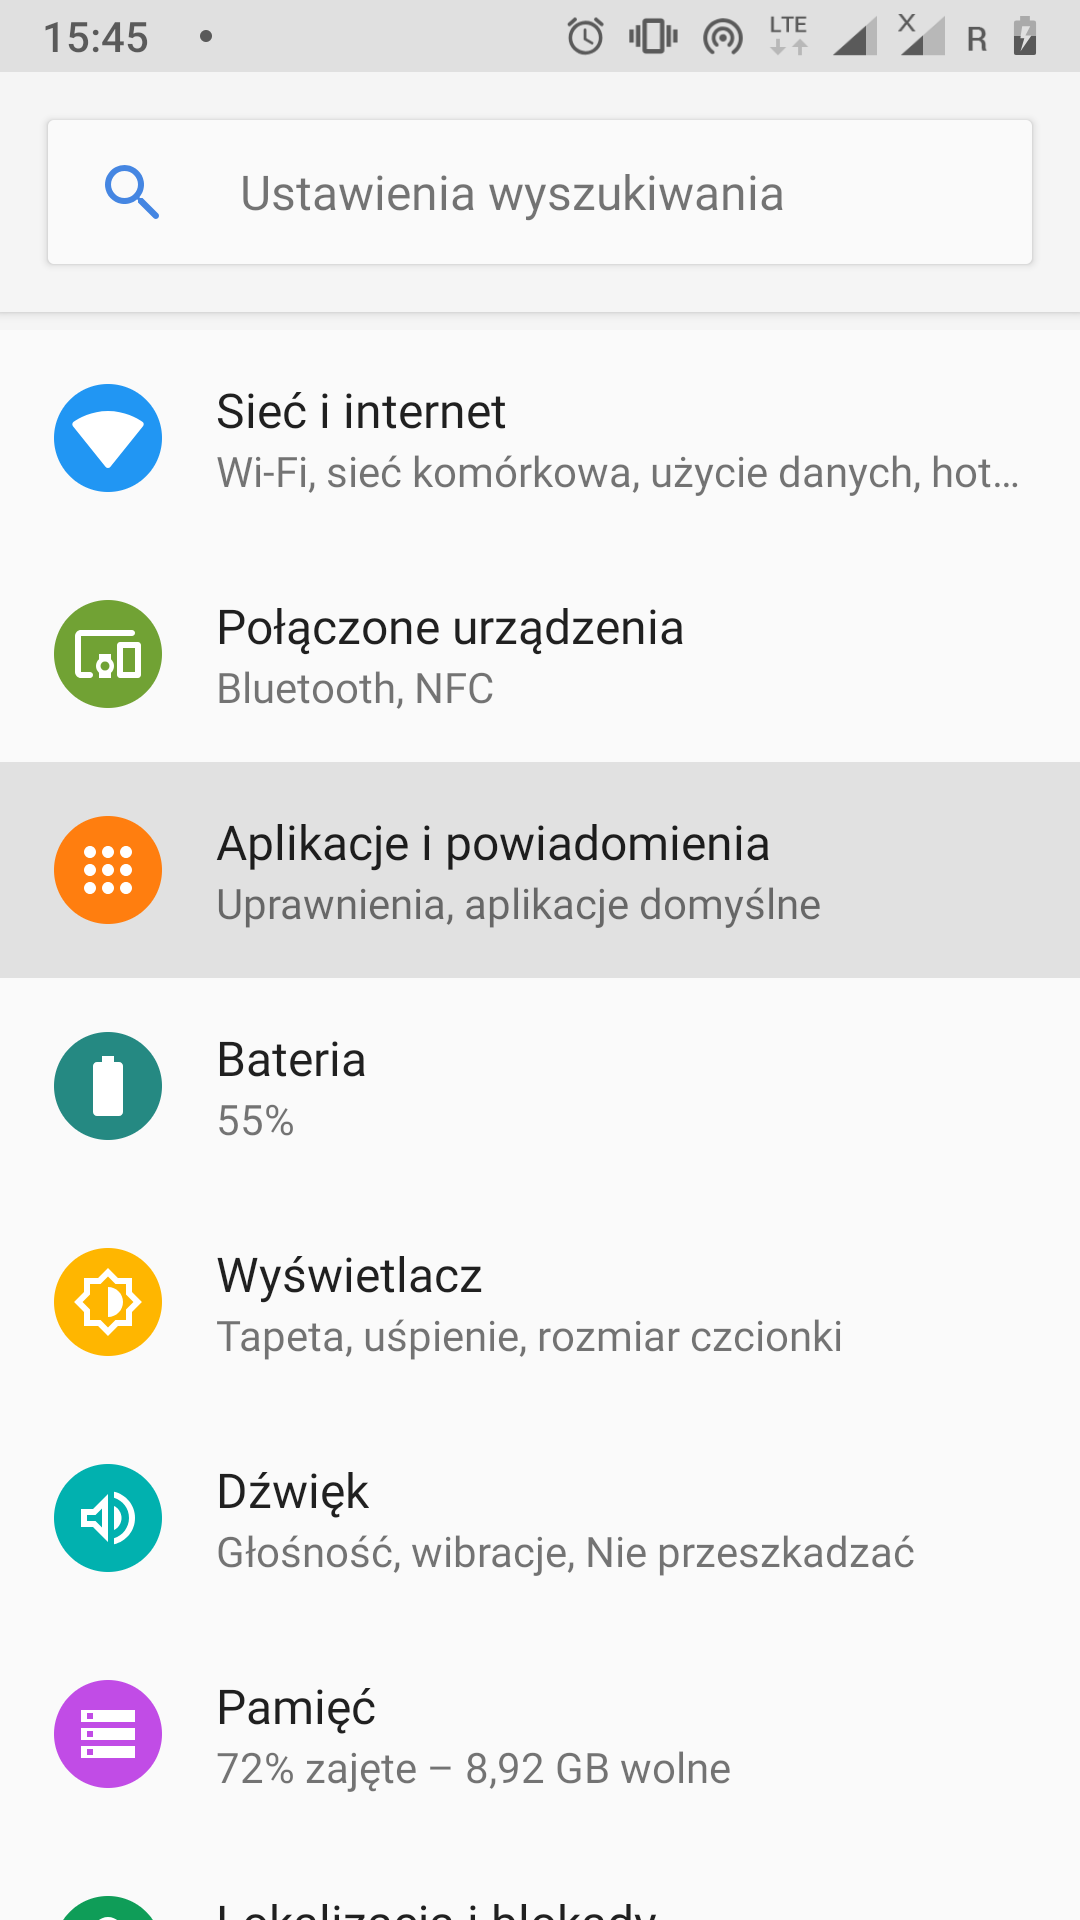
\includegraphics[scale=0.13]{dodatekA/1_1.png}
			\subcaption{\label{subfigure_a}}
		\end{subfigure}
		\begin{subfigure}{0.35\textwidth}
			\centering
			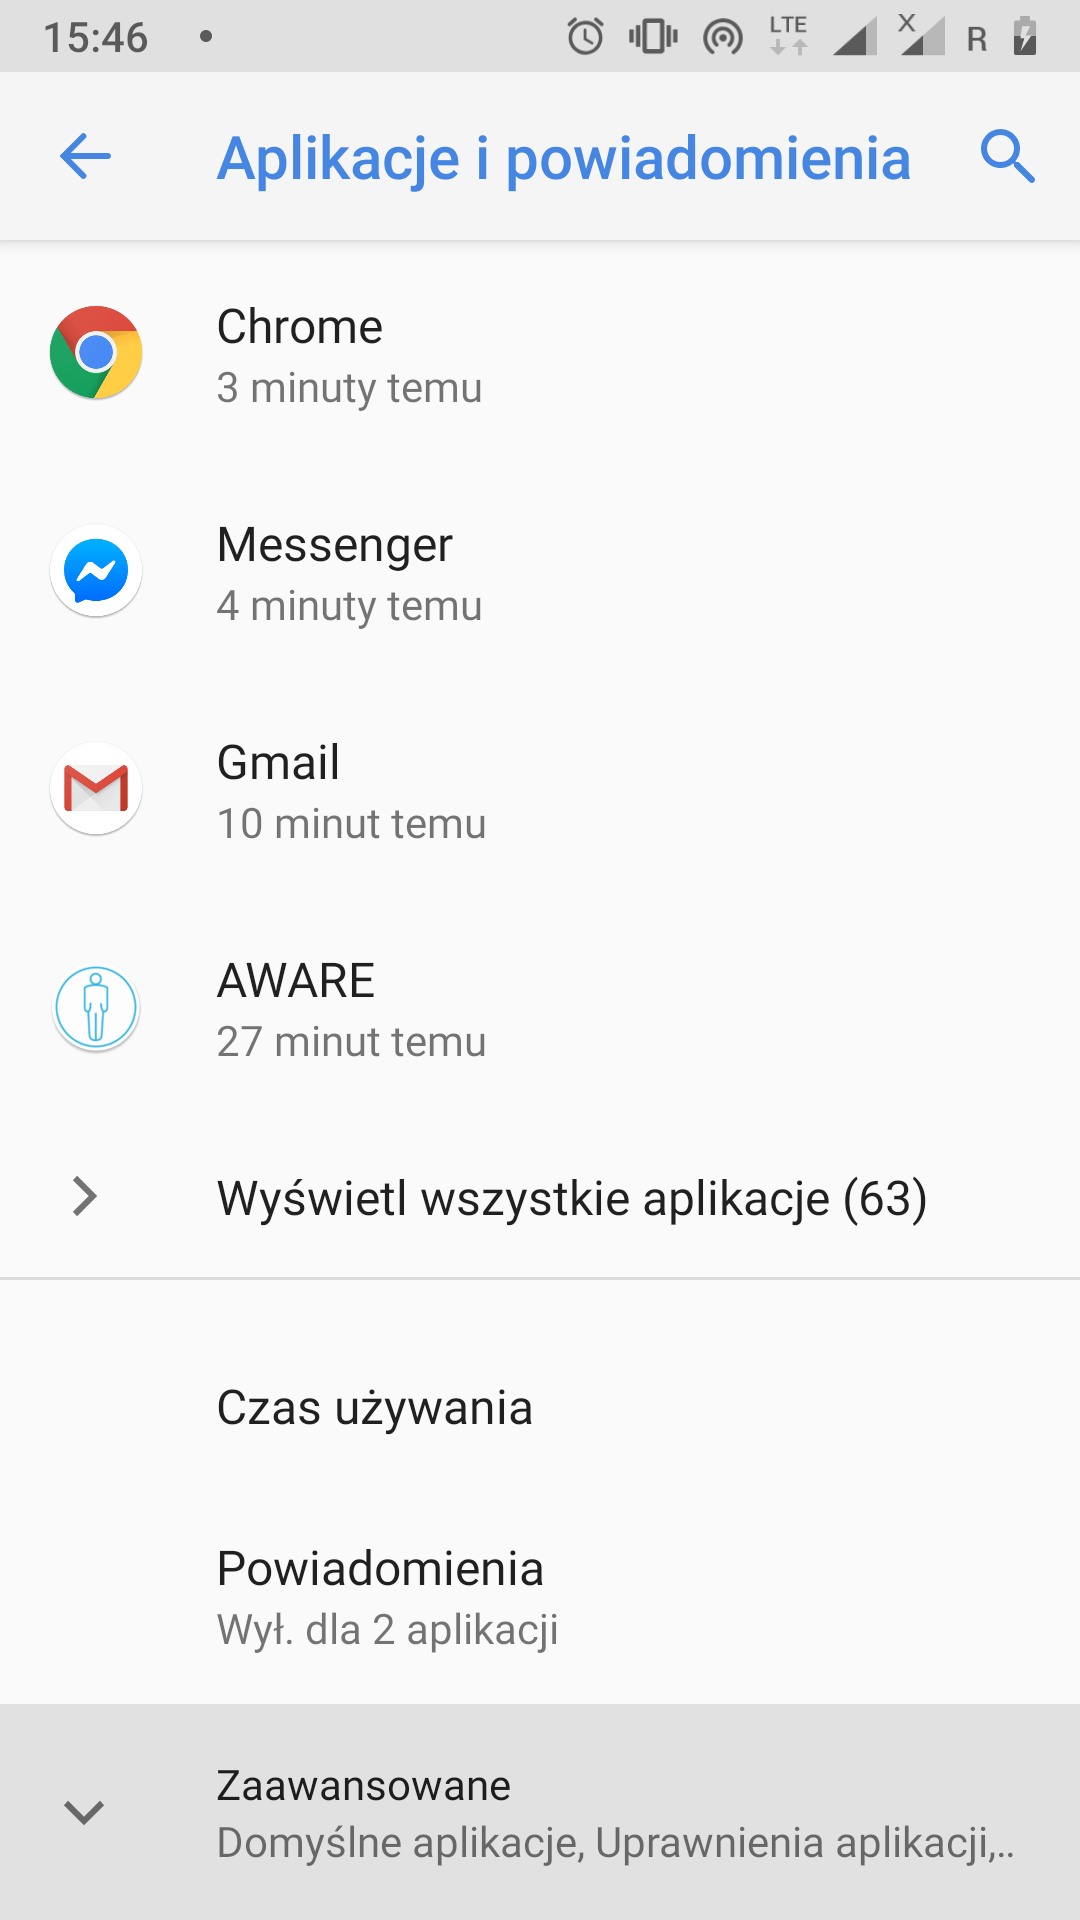
\includegraphics[scale=0.13]{dodatekA/1_2.png}
			\subcaption{\label{subfigure_b}}
		\end{subfigure}
		\caption{ Kroki 1 i 2: Przejście do zaawansowanych ustawień aplikacji.}
	\end{figure}
	
	
	\begin{figure}[H]
		\centering
		\begin{subfigure}{0.35\textwidth}
			\centering
			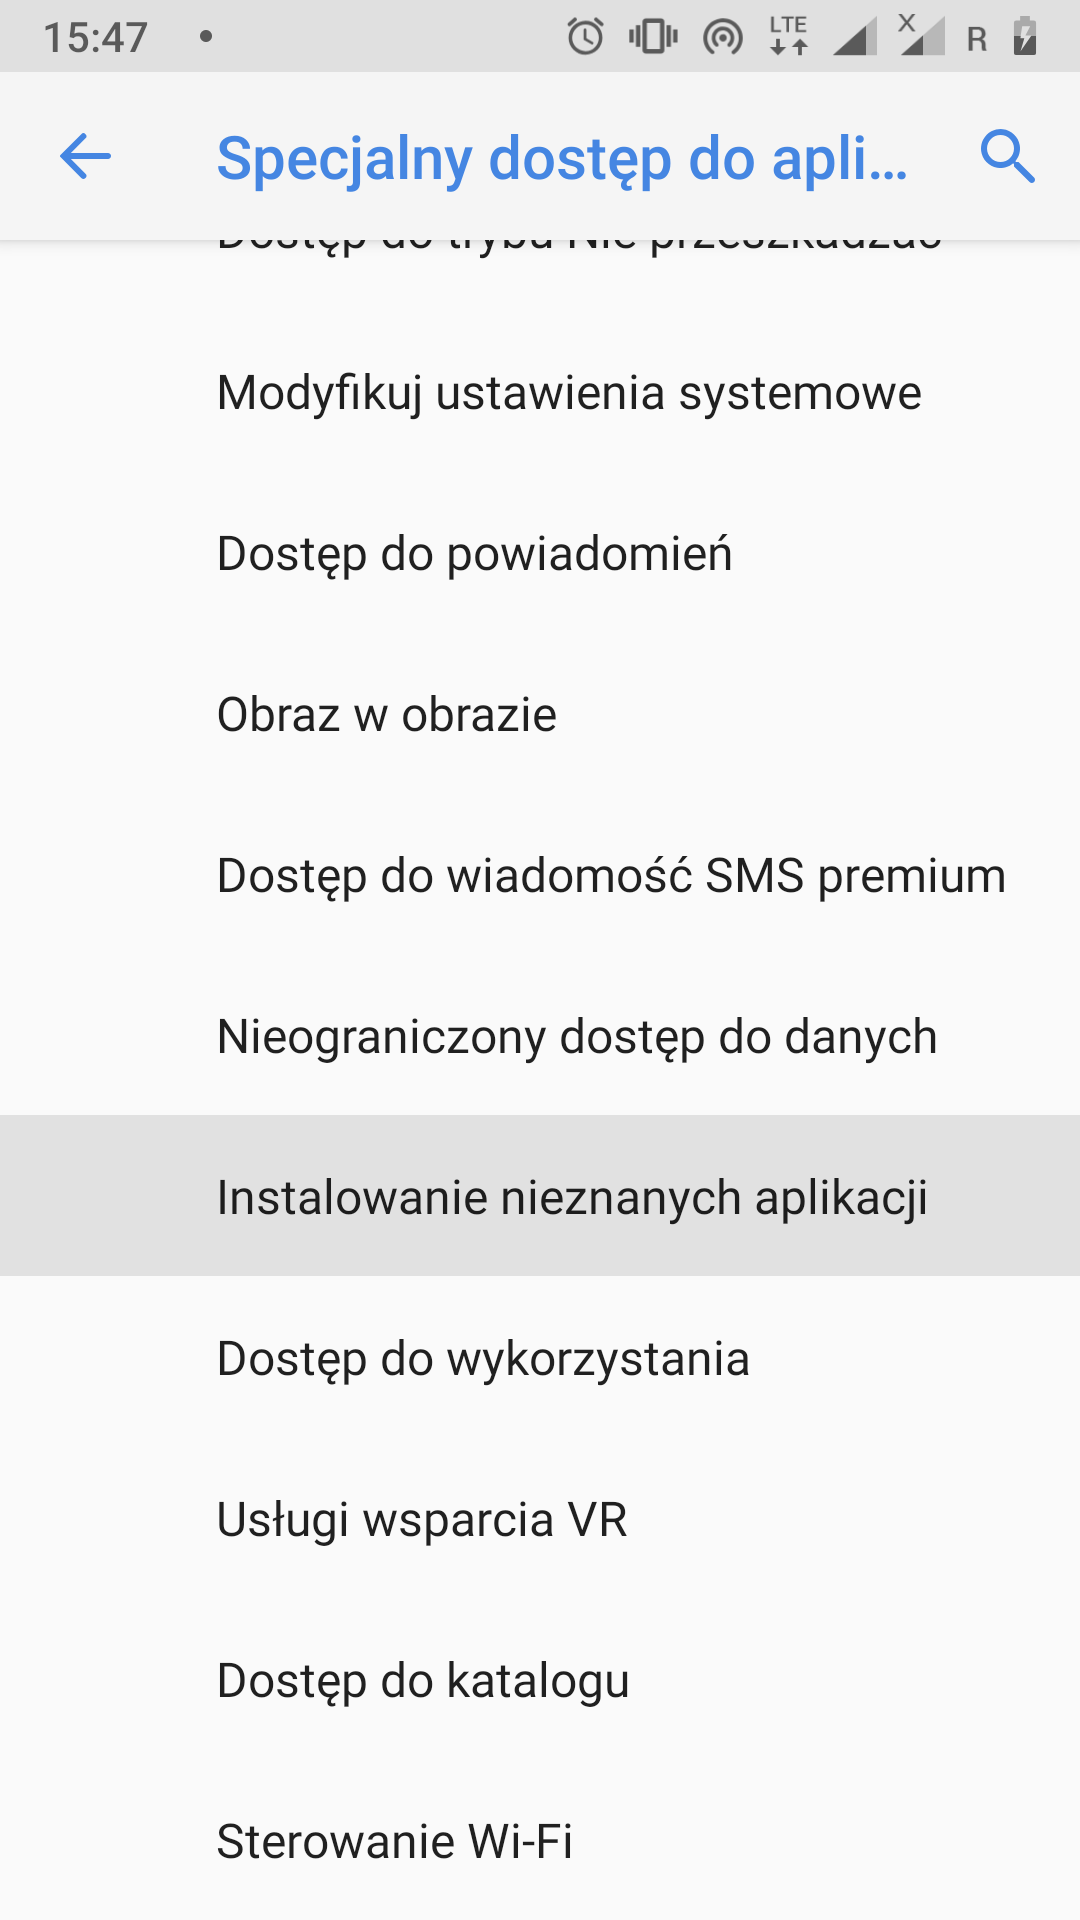
\includegraphics[scale=0.13]{dodatekA/1_3.png}
			\subcaption{\label{subfigure_a}}
		\end{subfigure}
		\begin{subfigure}{0.35\textwidth}
			\centering
			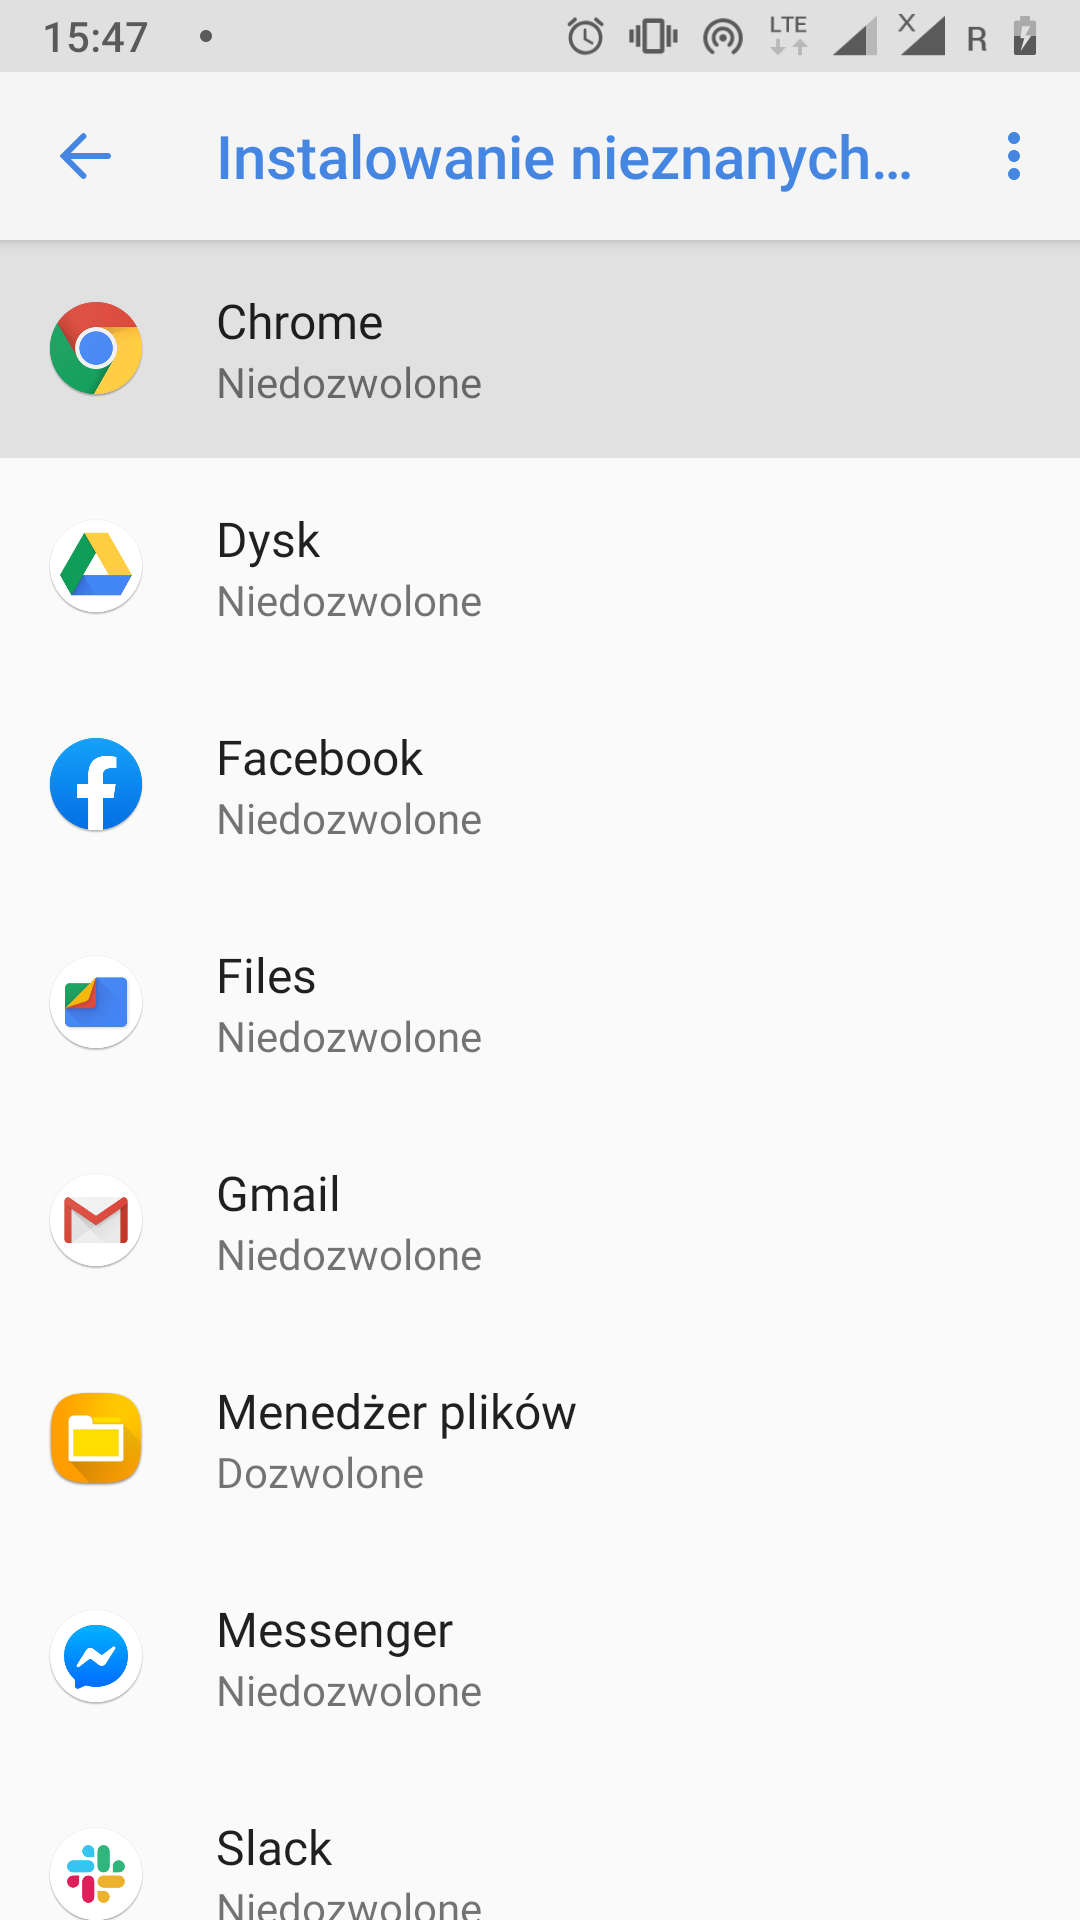
\includegraphics[scale=0.13]{dodatekA/1_4.png}
			\subcaption{\label{subfigure_b}}
		\end{subfigure}
		\caption{ Kroki 3 i 4: Aktywność \textit{Specjalny dostęp do aplikacji} (a) oraz aktywność \textit{Instalowanie nieznanych aplikacji} (b).}
	\end{figure}
	\clearpage 
	
	\begin{figure}[H]
		\centering
		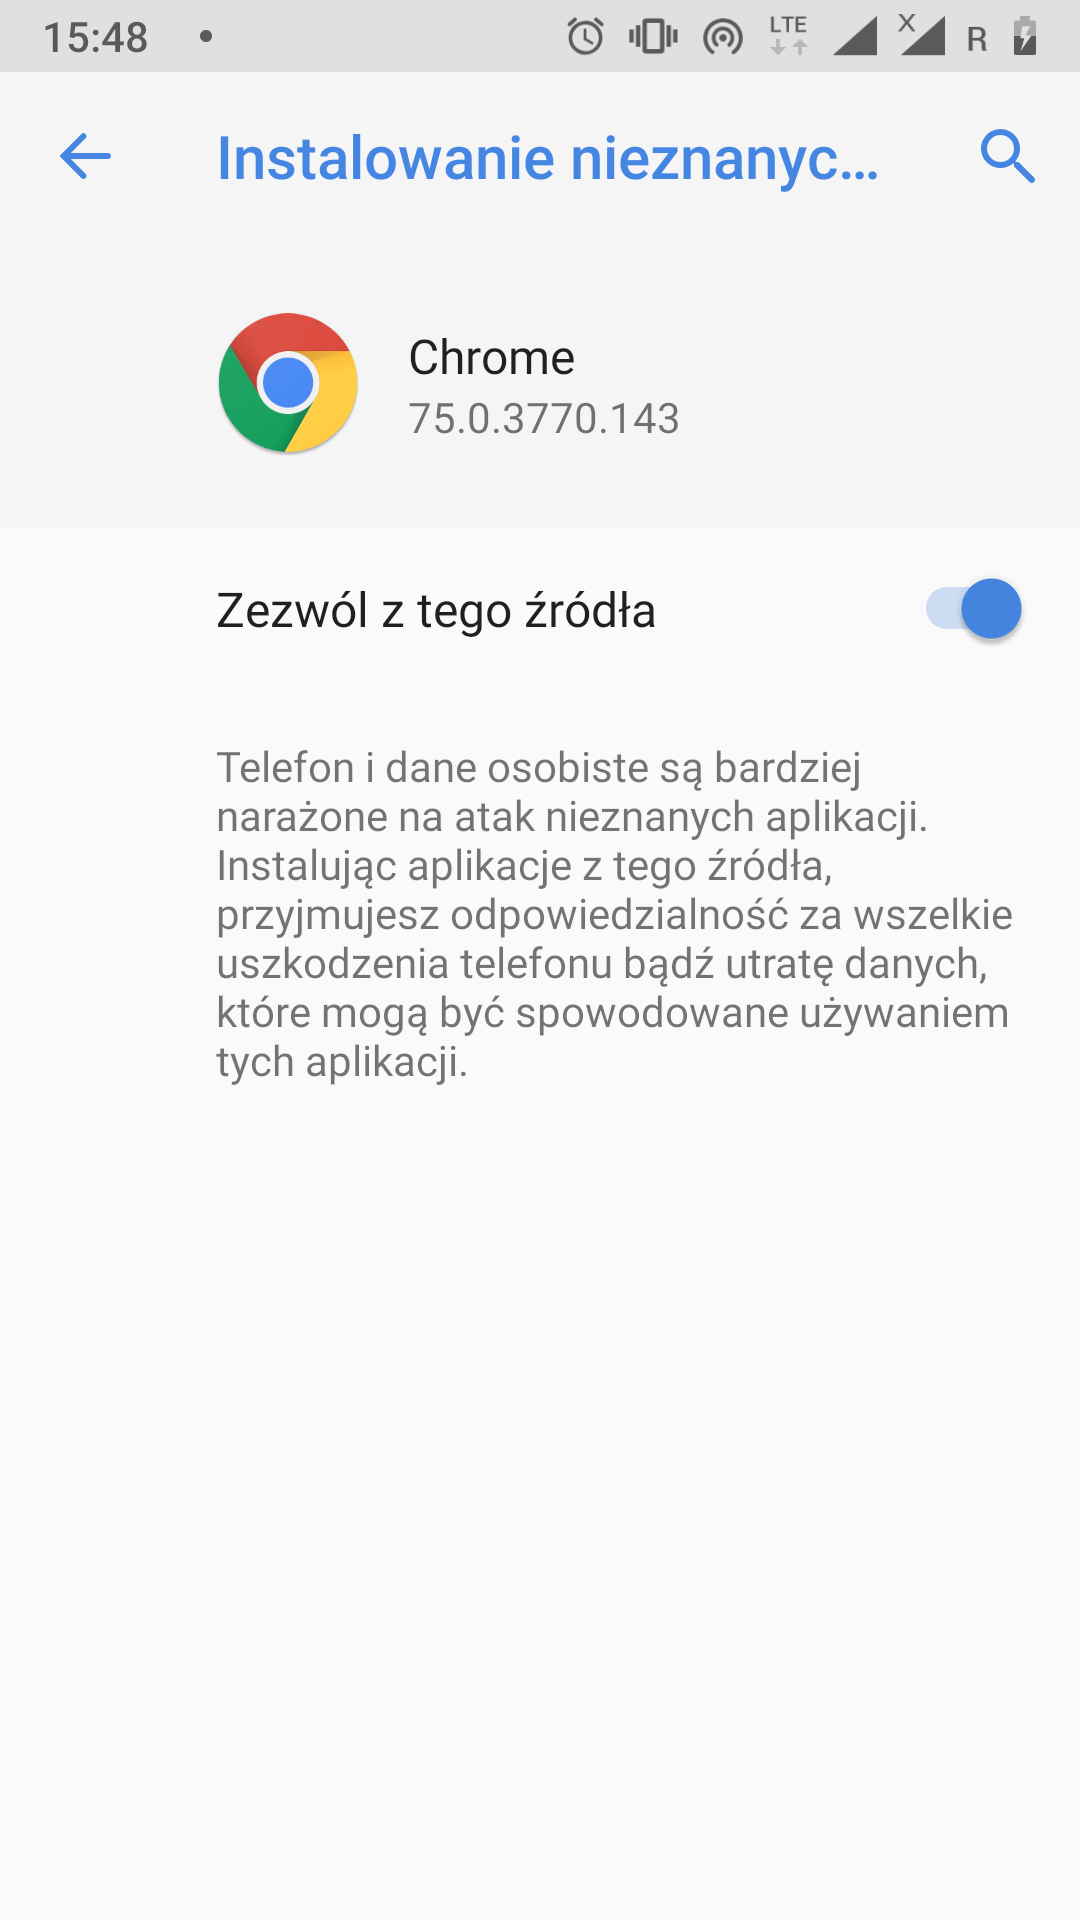
\includegraphics[scale=0.13]{dodatekA/1_5.png}
		\caption{Krok 5: Aktywność ustawień aplikacji.}
	\end{figure}
	
\end{enumerate}

%---------------------------------------------------------------------------

\section{Etap 2: Pobranie i instalacja aplikacji}
\label{sec:pobranieIInstalacjaAplikacji}

Następnie pobierzemy i zainstalujemy aplikacje potrzebne do przeprowadzenia badania.

\begin{enumerate}
	
	\item W przeglądarce telefonu, którą wybrałeś w~poprzednim kroku, odwiedź stronę \url{tiny.cc/97tz9y} lub \url{https://github.com/filipbiernat/HowAreYou_plugin/wiki/Linki-do-instalacji-HowAreYou}.
	
	\item Pobierz plik instalatora klikając na \textit{AwareClient}.
	
	\item Przeglądarka powiadomi Cię o pobraniu pakietu. Kliknij \textit{Otwórz}. 
	
	\item Rozpocznie się instalacja aplikacji. Kliknij \textit{Instaluj}.
	
	\clearpage 
	\begin{figure}[H]
		\centering
		\begin{subfigure}{0.35\textwidth}
			\centering
			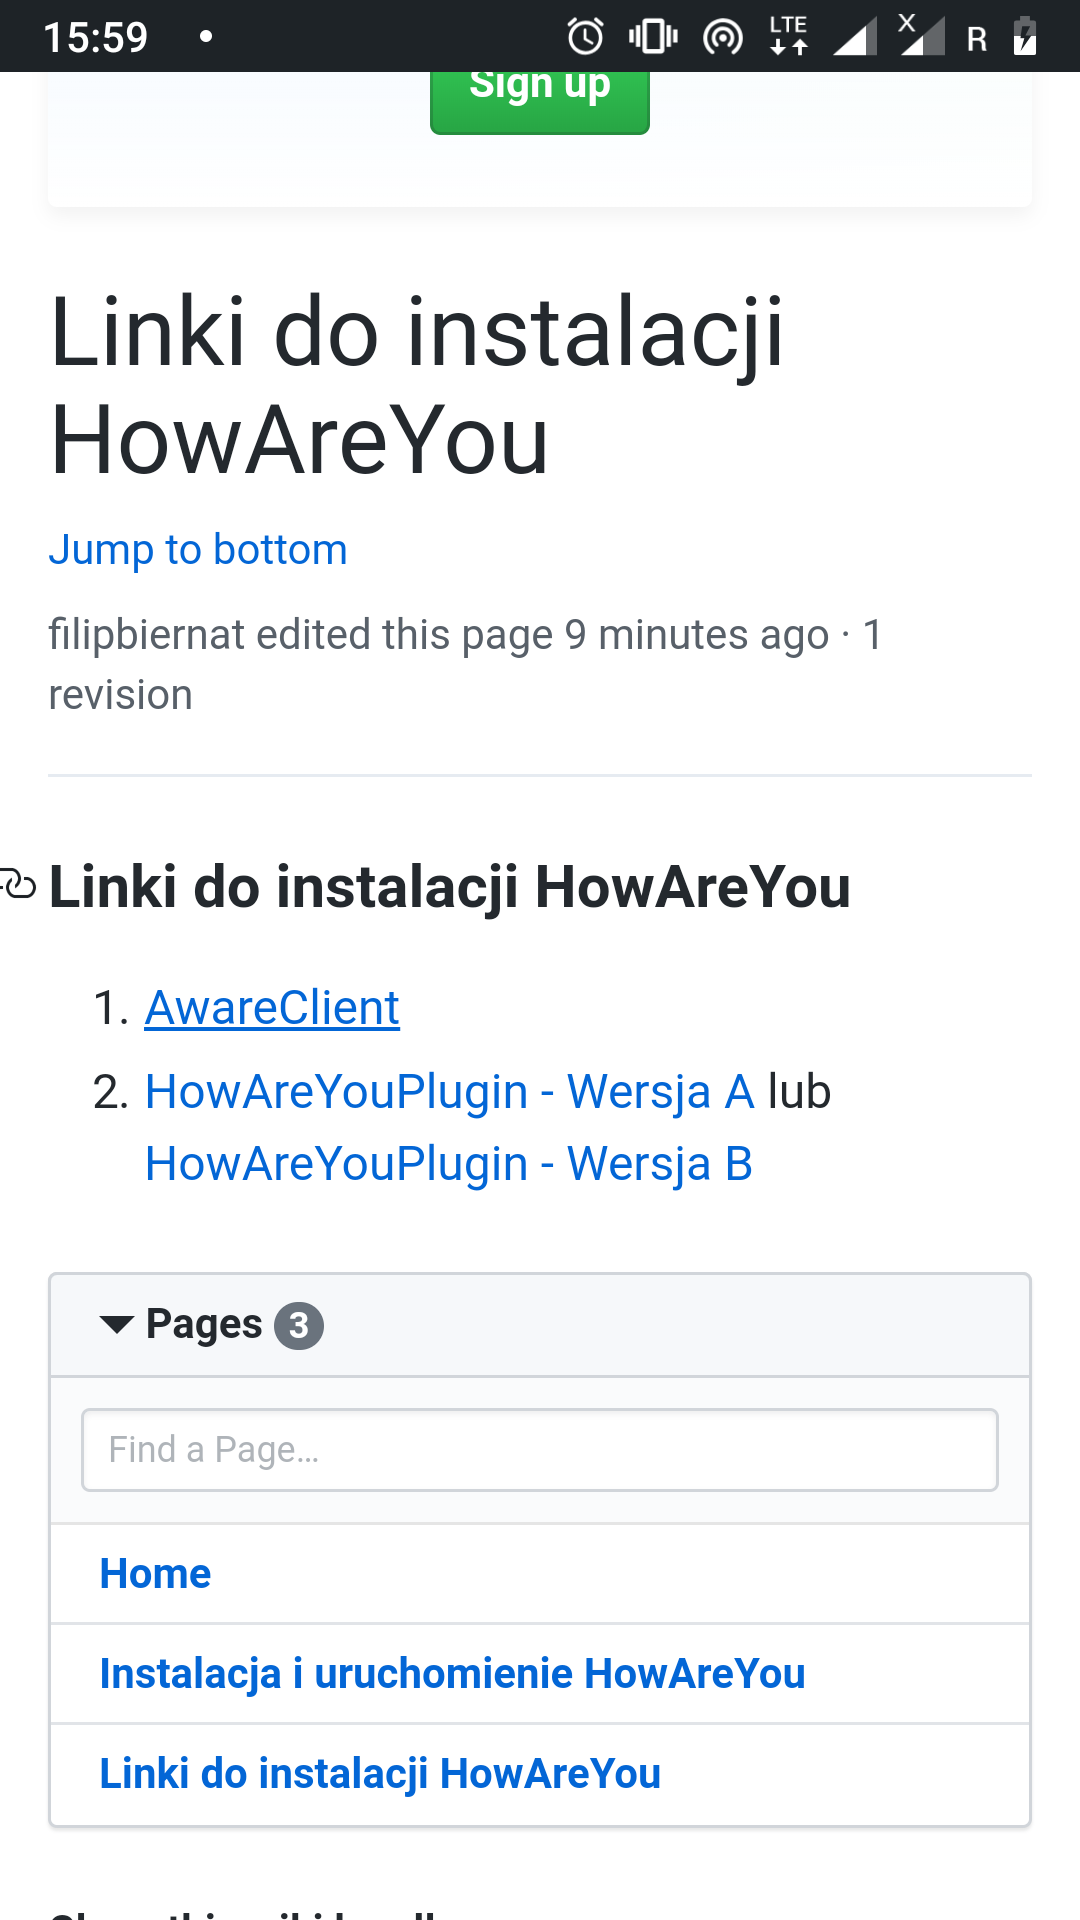
\includegraphics[scale=0.13]{dodatekA/2_1.png}
			\subcaption{\label{subfigure_a}}
		\end{subfigure}
		\begin{subfigure}{0.35\textwidth}
			\centering
			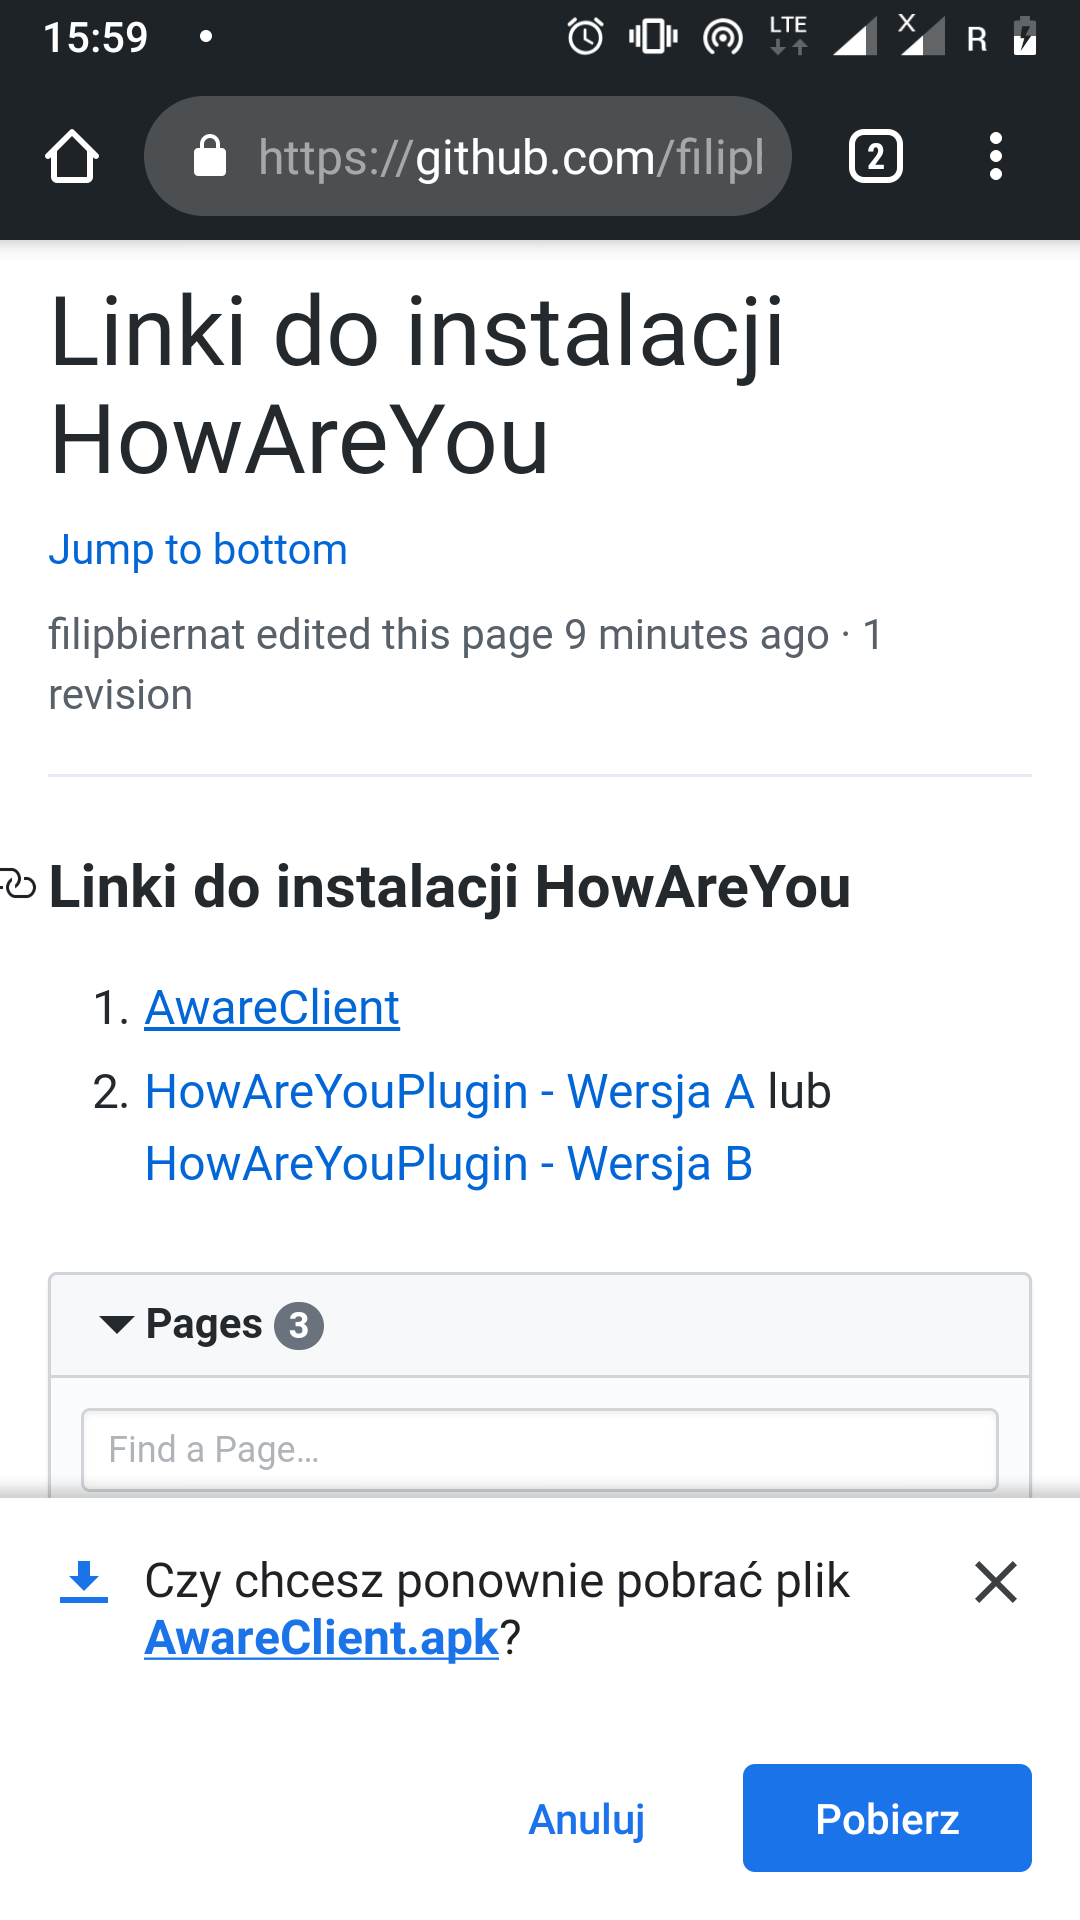
\includegraphics[scale=0.13]{dodatekA/2_2.png}
			\subcaption{\label{subfigure_b}}
		\end{subfigure}
		\caption{ Kroki 1 i 2: Strona www z~linkami umożliwiającymi pobranie aplikacji (a) oraz rozpoczęty proces pobierania aplikacji (b).}
	\end{figure}
	
	\begin{figure}[H]
		\centering
		\begin{subfigure}{0.35\textwidth}
			\centering
			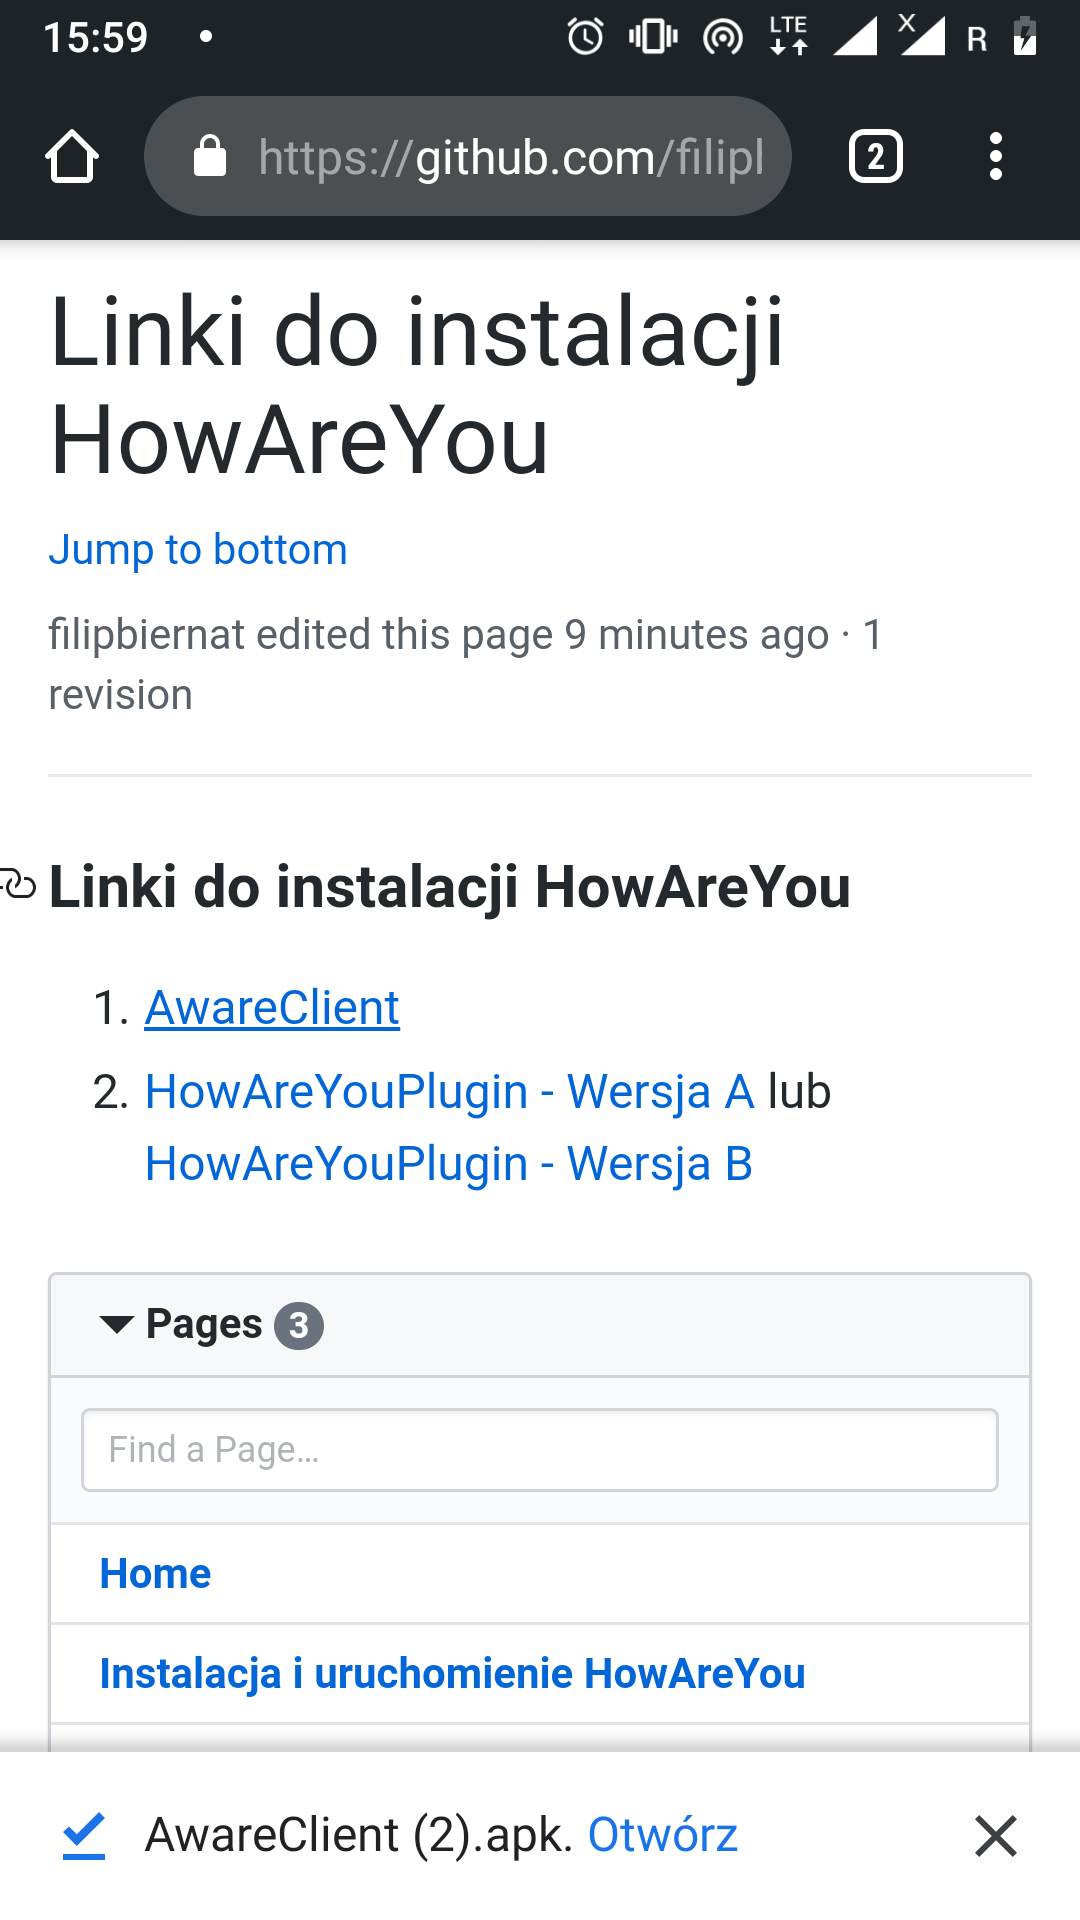
\includegraphics[scale=0.13]{dodatekA/2_3.png}
			\subcaption{\label{subfigure_a}}
		\end{subfigure}
		\begin{subfigure}{0.35\textwidth}
			\centering
			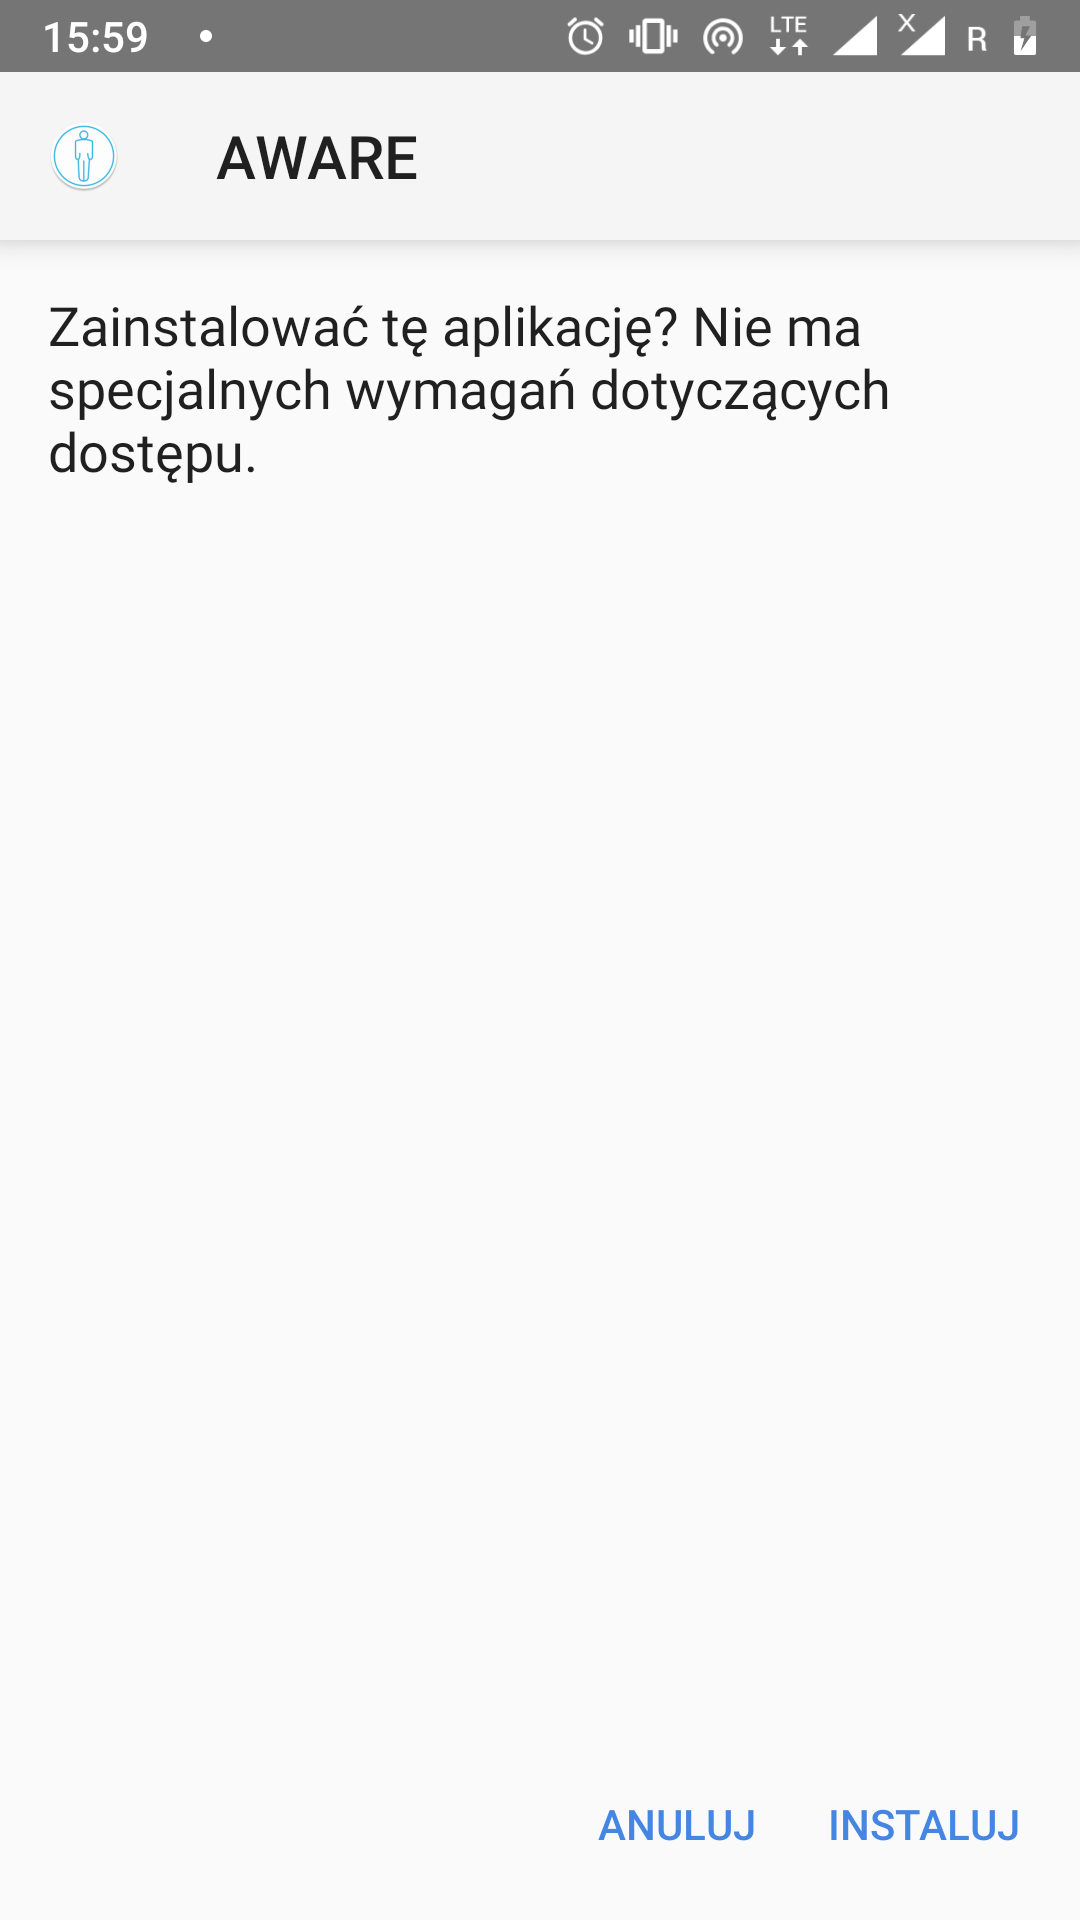
\includegraphics[scale=0.13]{dodatekA/2_4.png}
			\subcaption{\label{subfigure_b}}
		\end{subfigure}
		\caption{ Kroki 3 i 4: Wybór przycisków \textit{Otwórz} (a) oraz \textit{Instaluj} (b).}
	\end{figure}
	\clearpage 
	
	\item Po zakończeniu instalacji kliknij \textit{Gotowe} i powróć do przeglądarki.
	
	\item Przed rozpoczęciem badania zostałeś poproszony o pobranie wersji A lub wersji B aplikacji. Upewnij się którą wersję powinieneś wykorzystać.
	
	\item Pobierz plik instalatora klikając na \textit{HowAreYouPlugin - Wersja A} lub \textit{HowAreYouPlugin - Wersja B}.
	
	\item Podobnie jak wcześniej, kliknij \textit{Otwórz}. Rozpocznie się instalacja aplikacji. Kliknij \textit{Instaluj}. 
	
	\item Ponownie kliknij przycisk \textit{Gotowe}. Zamknij przeglądarkę i powróć do ekranu głównego.
	
	\begin{figure}[H]
		\centering
		\begin{subfigure}{0.35\textwidth}
			\centering
			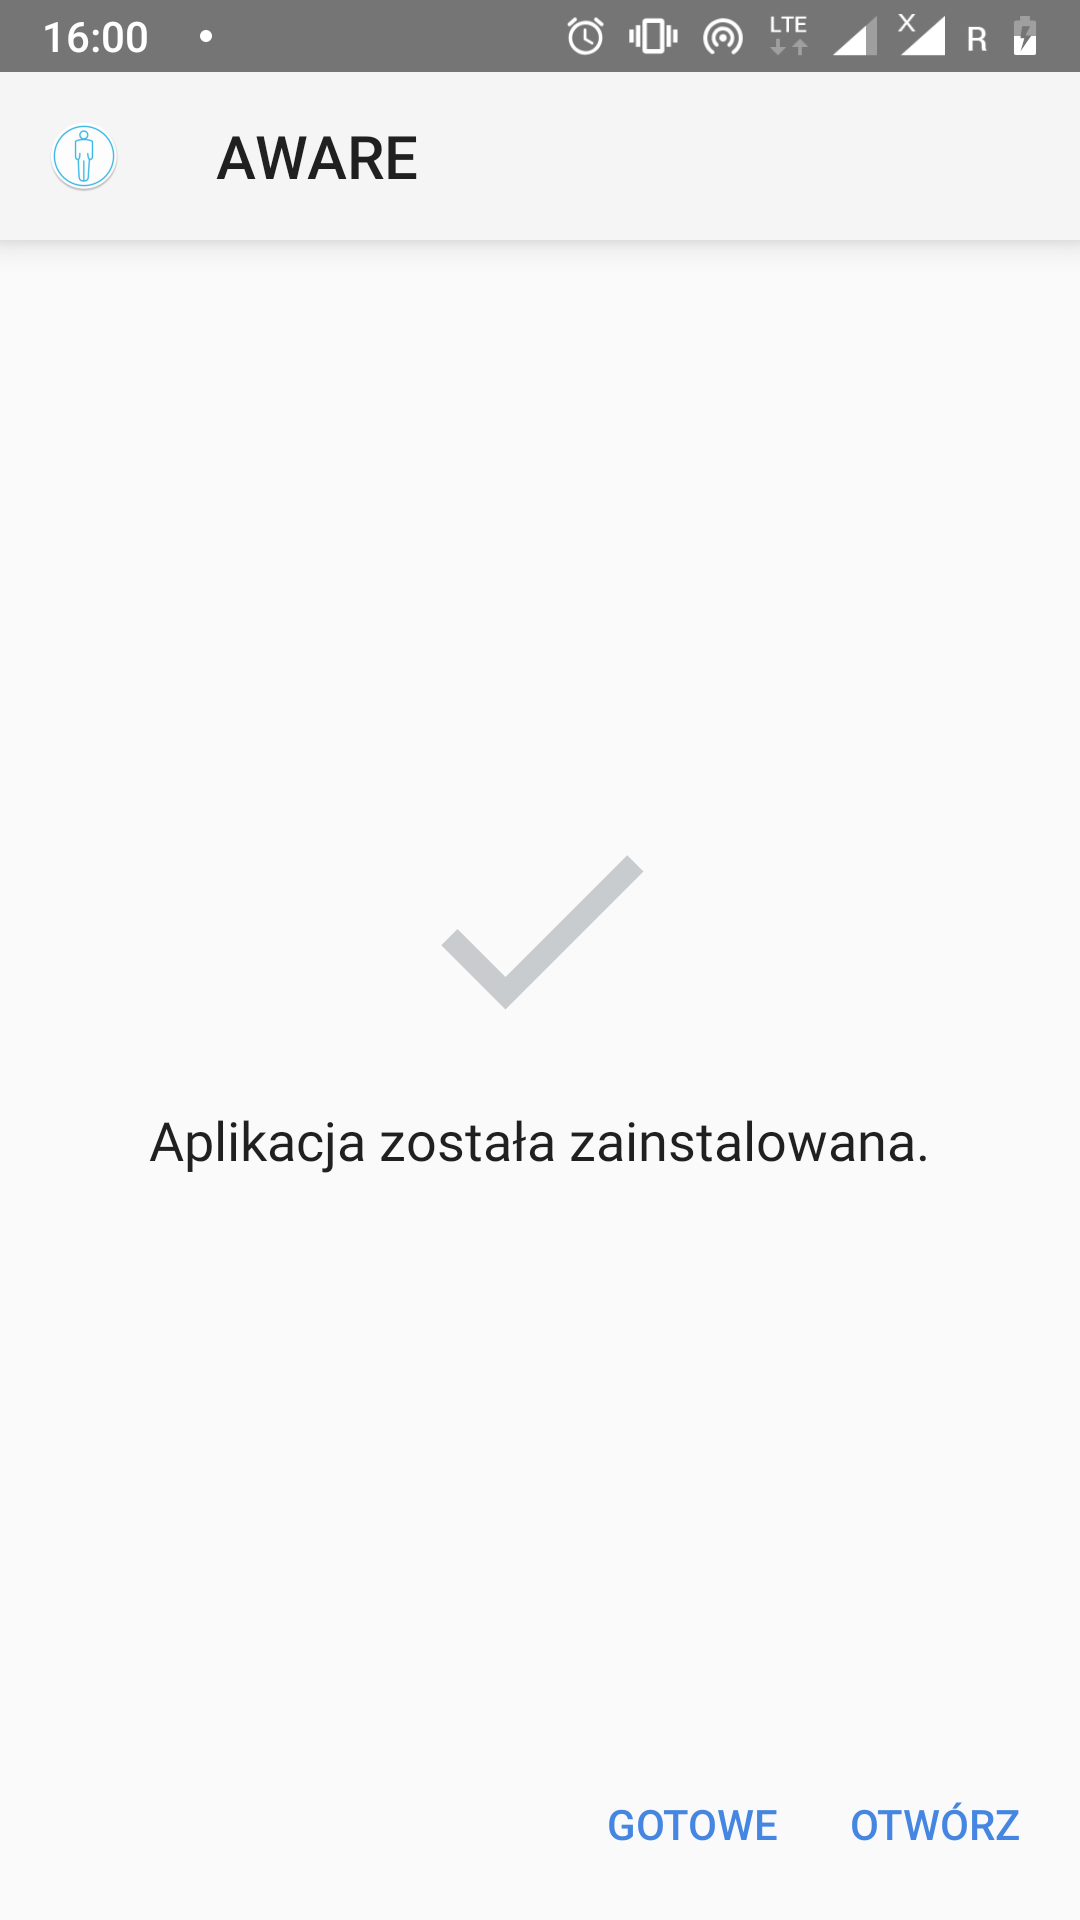
\includegraphics[scale=0.13]{dodatekA/2_5.png}
			\subcaption{\label{subfigure_a}}
		\end{subfigure}
		\begin{subfigure}{0.35\textwidth}
			\centering
			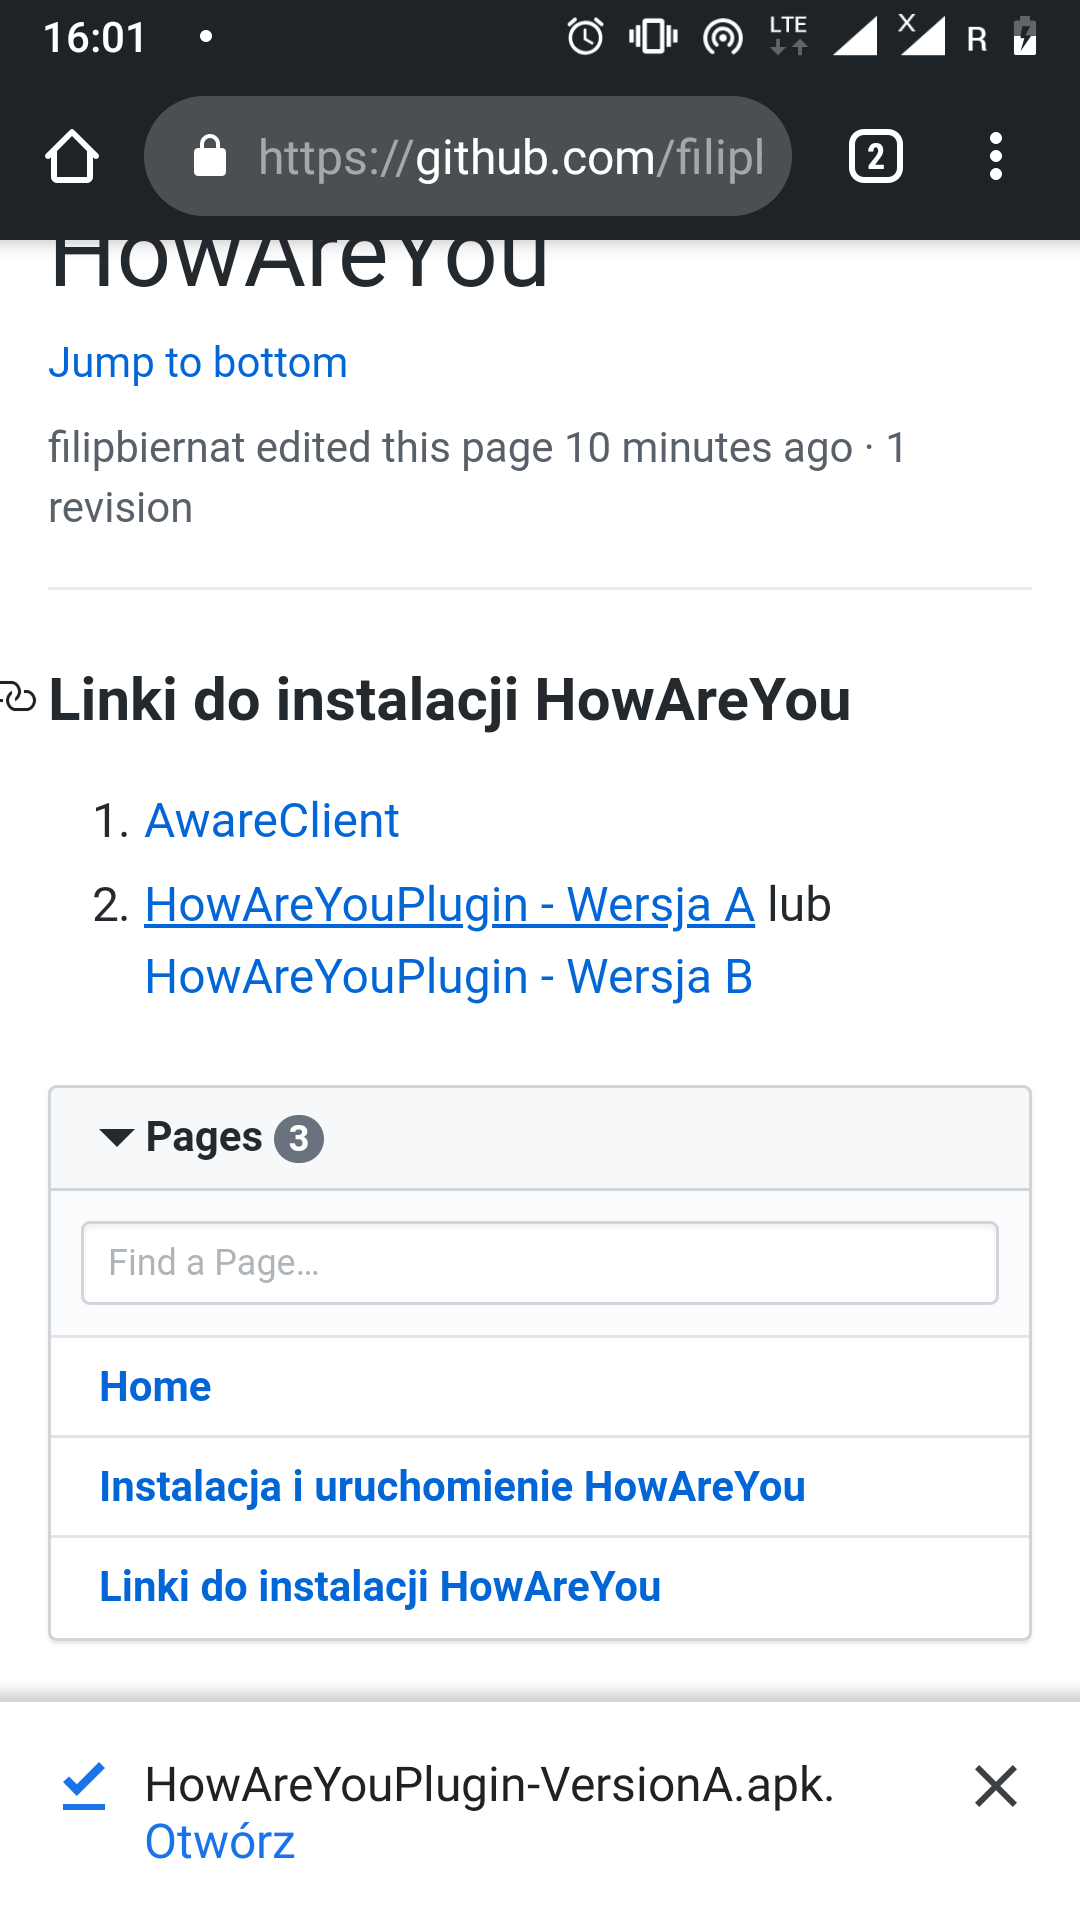
\includegraphics[scale=0.13]{dodatekA/2_7.png}
			\subcaption{\label{subfigure_b}}
		\end{subfigure}
		\caption{ Kroki 5 i 7: Wybór przycisku \textit{Gotowe} (a) oraz wybór wersji pluginu (b).}
	\end{figure}
	\clearpage
	
	\begin{figure}[H]
		\centering
		\begin{subfigure}{0.35\textwidth}
			\centering
			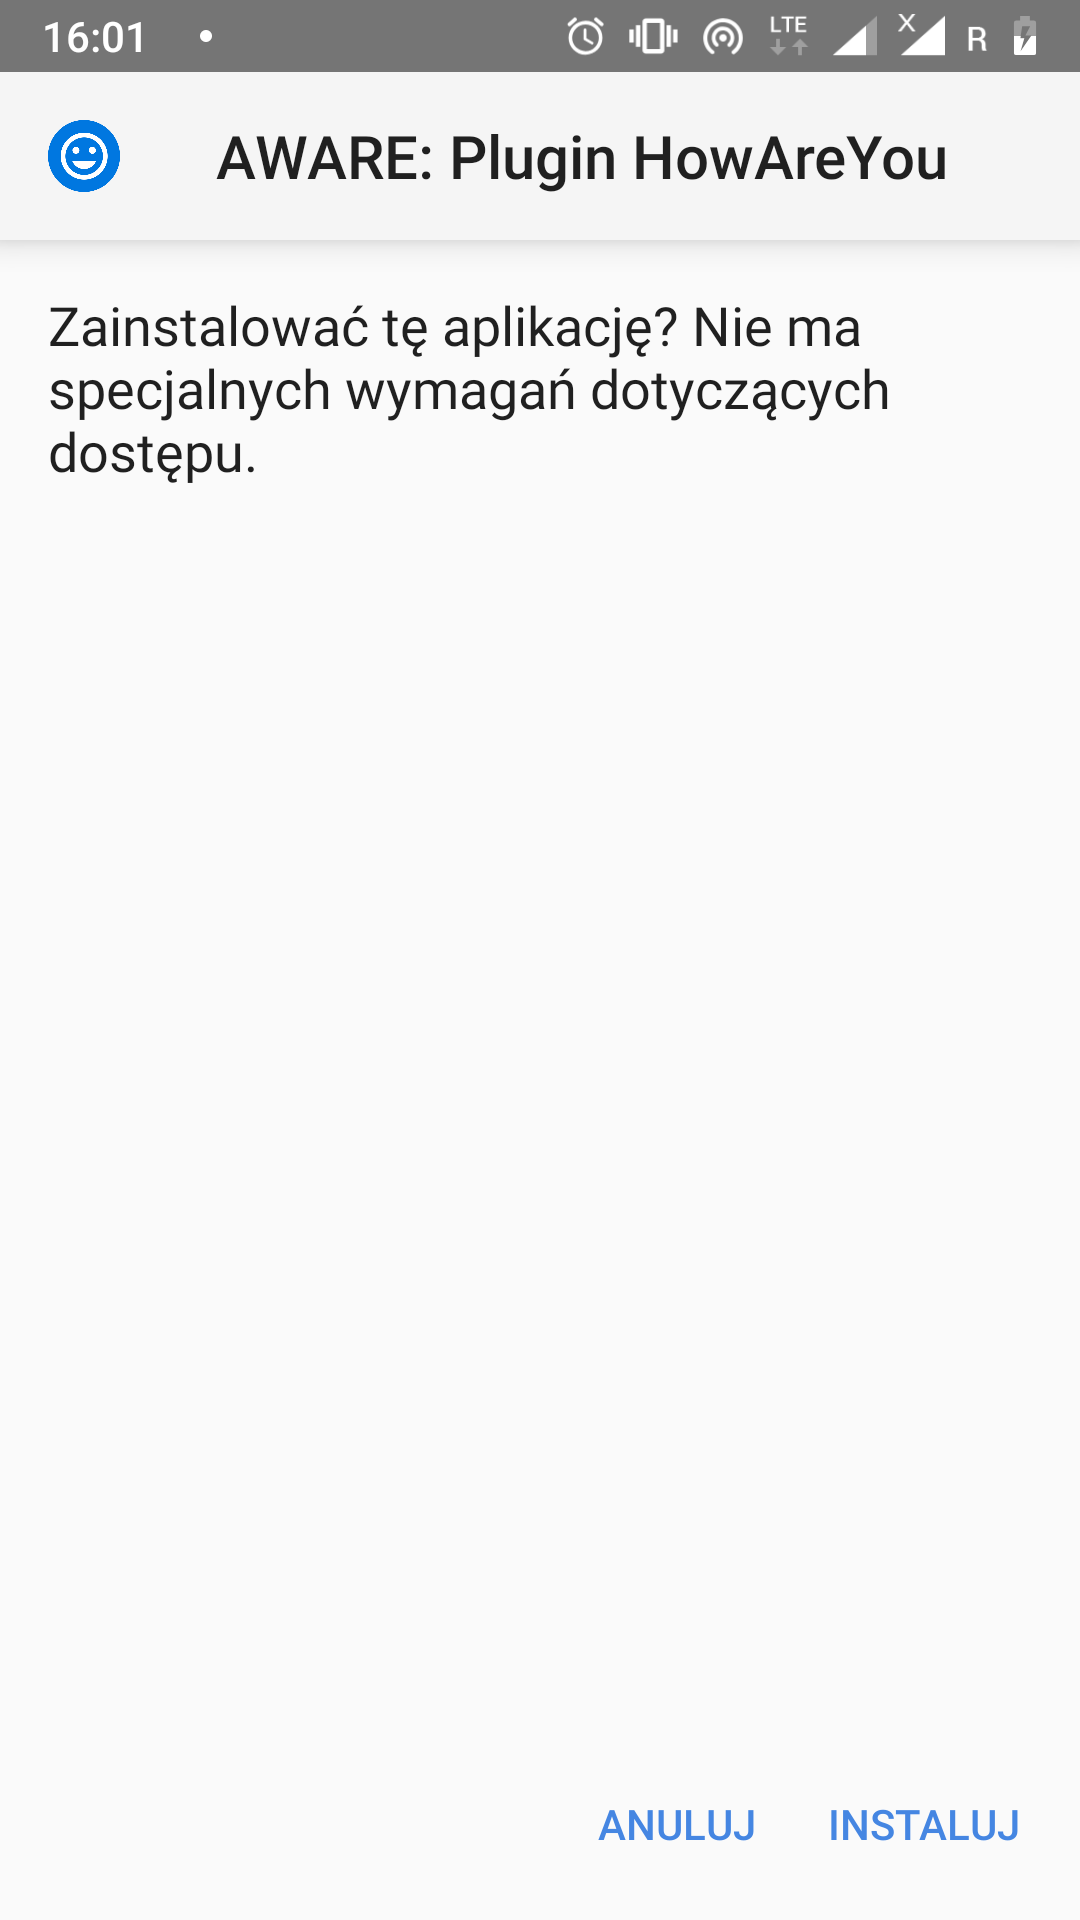
\includegraphics[scale=0.13]{dodatekA/2_8.png}
			\subcaption{\label{subfigure_a}}
		\end{subfigure}
		\begin{subfigure}{0.35\textwidth}
			\centering
			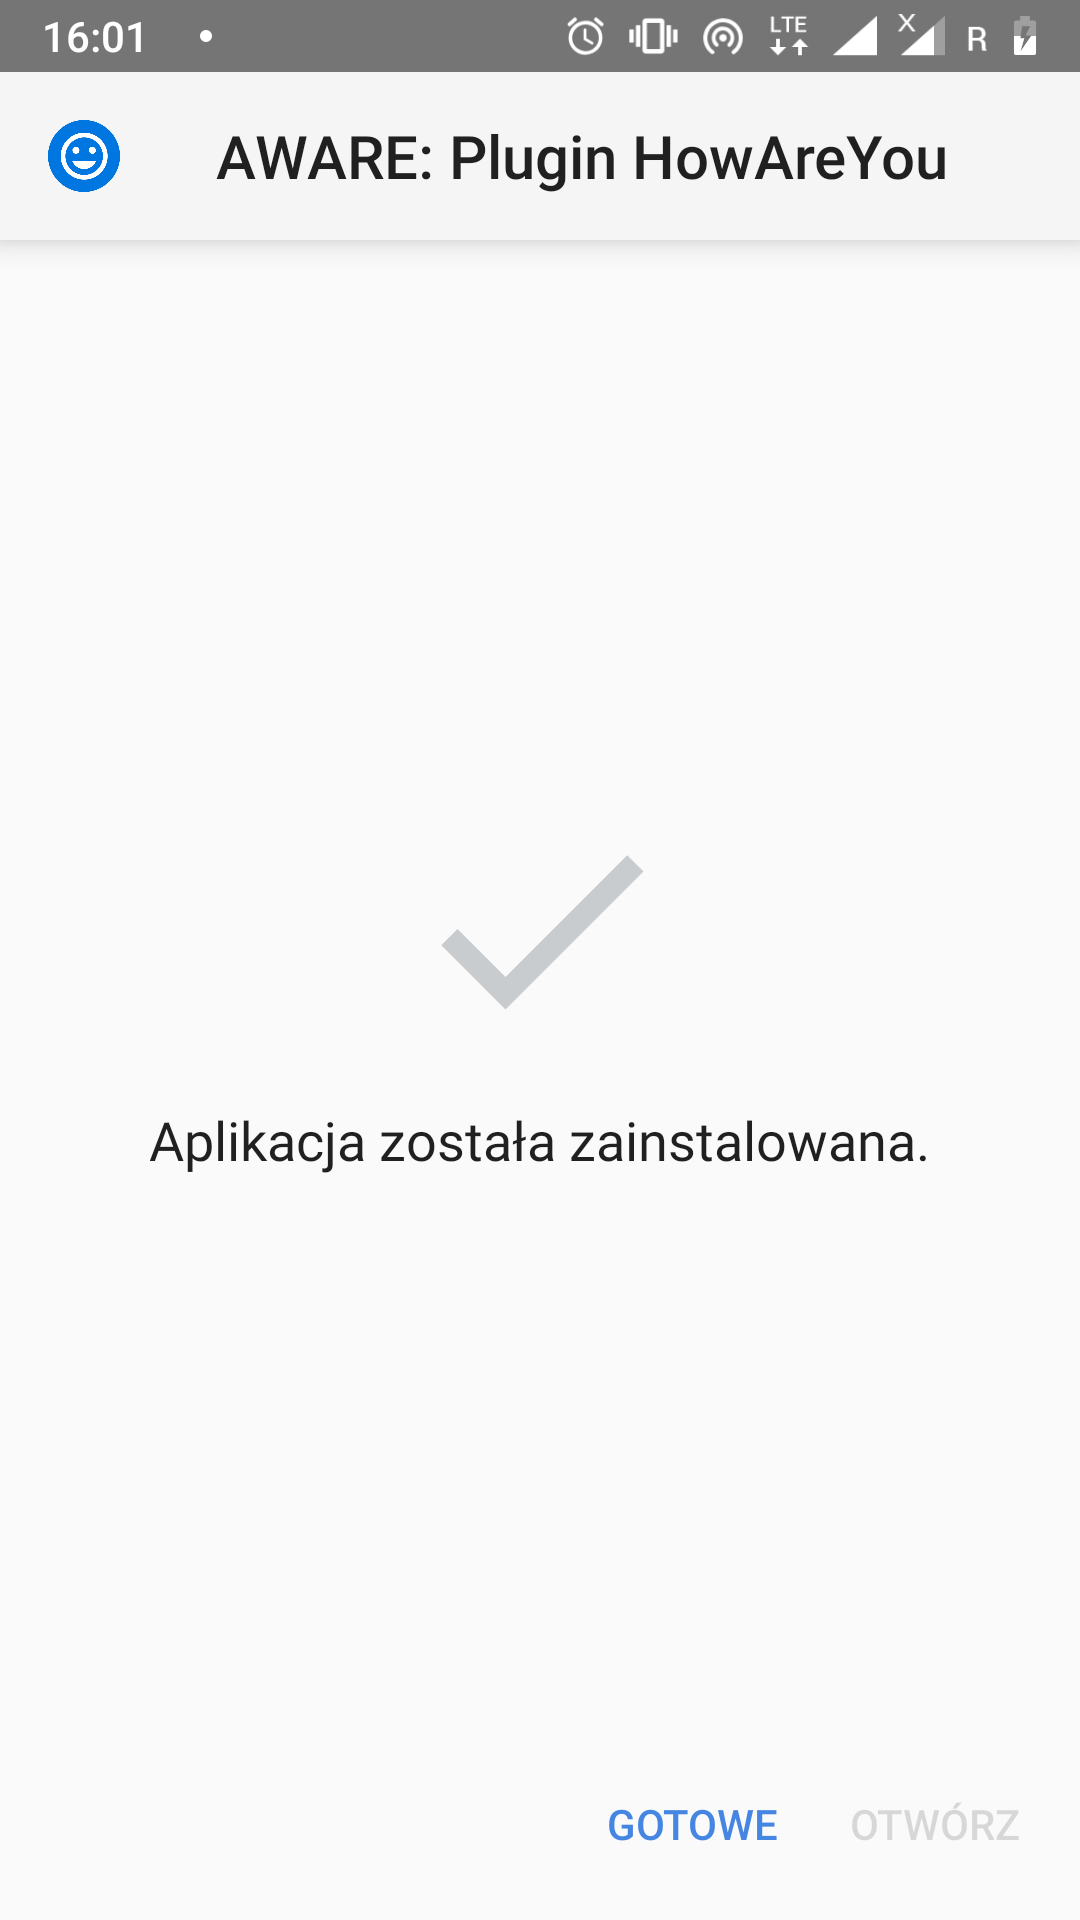
\includegraphics[scale=0.13]{dodatekA/2_9.png}
			\subcaption{\label{subfigure_b}}
		\end{subfigure}
		\caption{ Kroki 8 i 9: Wybór przycisków \textit{Instaluj} (a) oraz \textit{Gotowe} (b).}
	\end{figure}
\end{enumerate}

%---------------------------------------------------------------------------

\section{Etap 3: Konfiguracja aplikacji}
\label{sec:pobranieIInstalacjaAplikacji}

Ostatnim krokiem będzie konfiguracja aplikacji klietna oraz pluginu \textit{HowAreYou}.

\begin{enumerate}
	
	\item Uruchom aplikację \textit{AWARE}.
	
	\item Zostaniesz zapytany o zgody na wykorzystanie zasobów telefonu. Zatwierdź odpowiednie zgody.
	
	\item W aplikacji przejdź do zakładki \textit{Plugins}.
	
	\item Wybierz plugin \textit{HowAreYou}. Jeżeli plugin nie jest jeszcze aktywny, kliknij \textit{Activate}.
	\clearpage
	
	\begin{figure}[H]
		\centering
		\begin{subfigure}{0.35\textwidth}
			\centering
			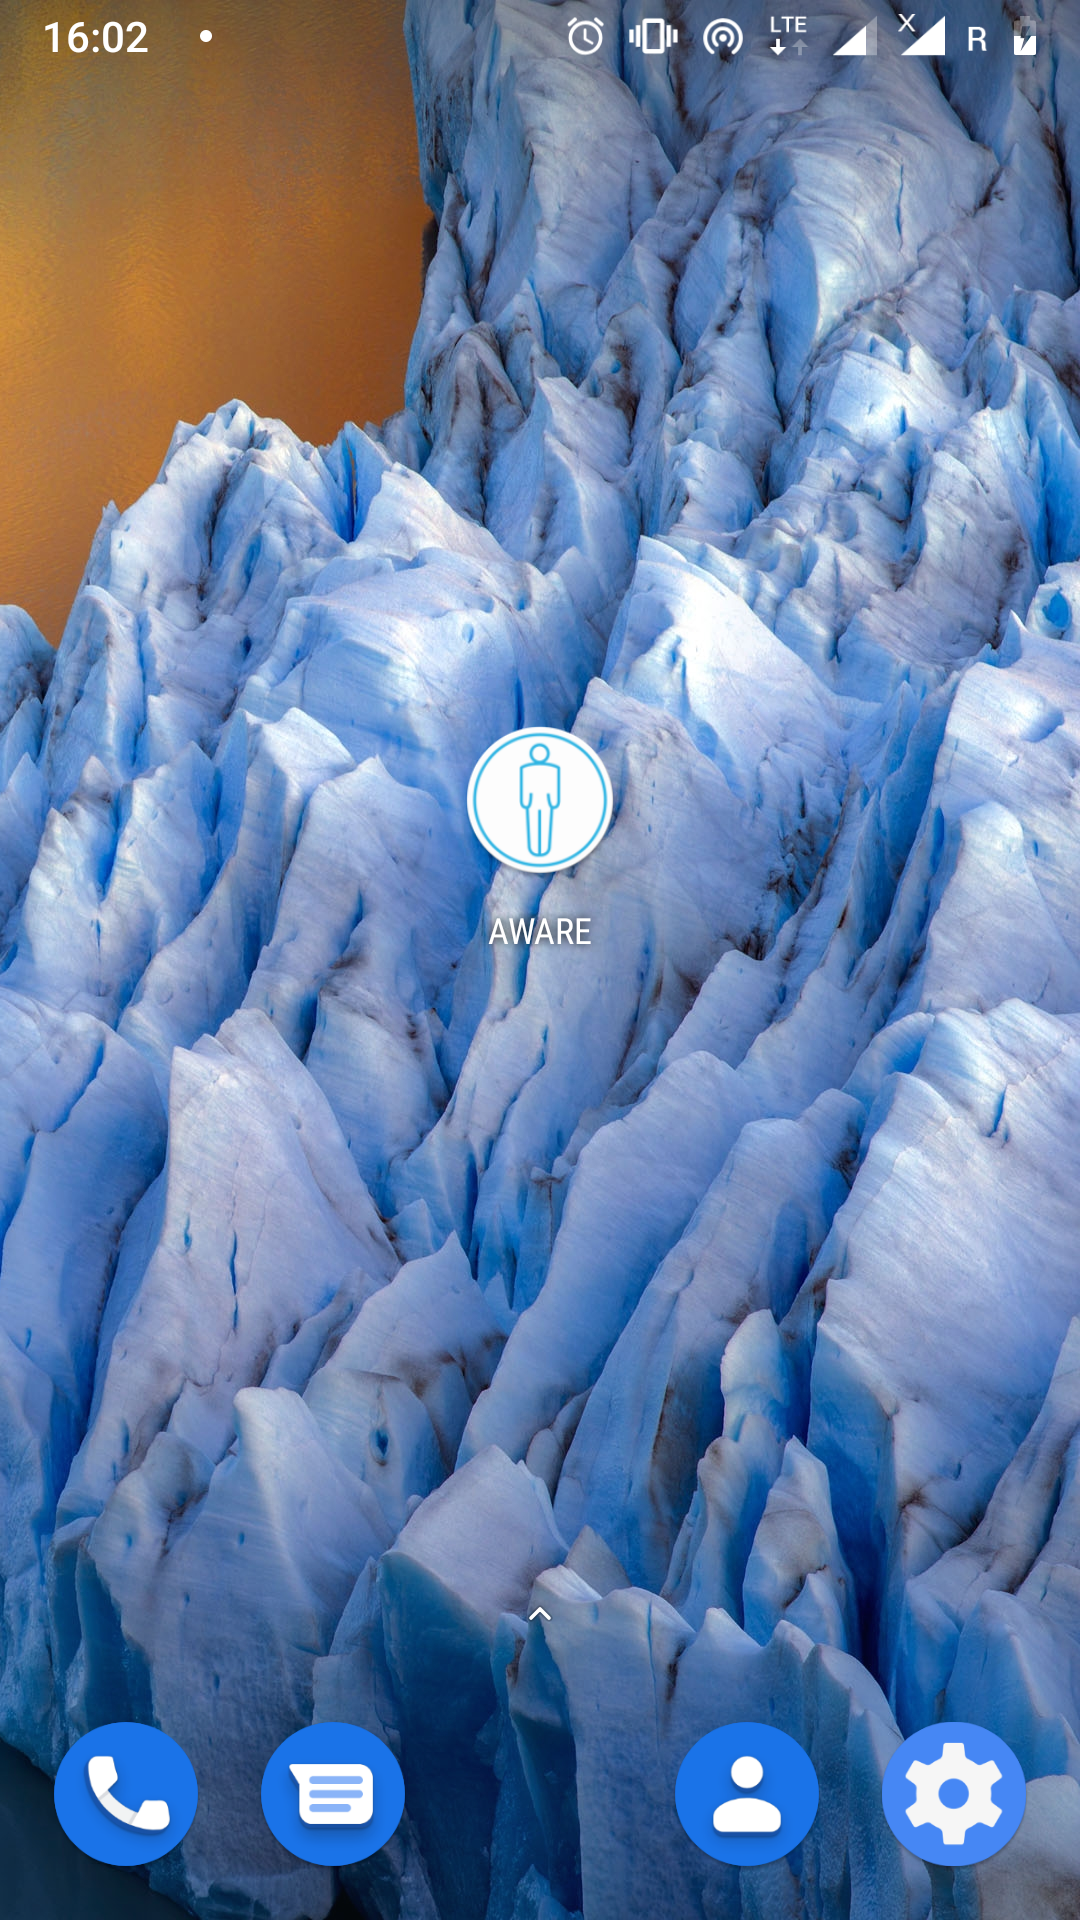
\includegraphics[scale=0.13]{dodatekA/3_1.png}
			\subcaption{\label{subfigure_a}}
		\end{subfigure}
		\begin{subfigure}{0.35\textwidth}
			\centering
			\includegraphics[scale=0.13]{dodatekA/3_2.png}
			\subcaption{\label{subfigure_b}}
		\end{subfigure}
		\caption{ Kroki 1 i 2: Uruchomienie aplikacji \textit{AWARE} (a) oraz widok zapytania użytkownika o zgodę (b).}
	\end{figure}
	
	\begin{figure}[H]
		\centering
		\begin{subfigure}{0.35\textwidth}
			\centering
			\includegraphics[scale=0.13]{dodatekA/3_3.png}
			\subcaption{\label{subfigure_a}}
		\end{subfigure}
		\begin{subfigure}{0.35\textwidth}
			\centering
			\includegraphics[scale=0.13]{dodatekA/3_4.png}
			\subcaption{\label{subfigure_b}}
		\end{subfigure}
		\caption{ Kroki 3 i 4: Widok listy dostępnych pluginów (a) oraz menu aktywacji pluginu (b).}
	\end{figure}
	\clearpage 
	
	\item Zostaniesz zapytany o zgody na wykorzystanie zasobów telefonu. Zatwierdź odpowiednie zgody.
	
	\item W systemie pojawi się powiadomienie \textit{Please enable AWARE}. Kliknij na obszar powiadomienia. Otworzy się okno \textit{Accessibility Service}.
	
	\item Kliknij na aplikację \textit{AWARE} i przyznaj uprawnienia klikając \textit{Użyj usługi}. Następnie kliknij na plugin \textit{HowAreYou} i przyznaj uprawnienia klikając \textit{Użyj usługi}.
	
	\item Jeżeli pojawi się powiadomienie \textit{Tap and add to the ignore battery optimizations' list}, kliknij na obszar powiadomienia.
	
	\item Wybierz \textit{Pokaż wszystkie aplikacje}.
	
	\item Zarówno na aplikacji \textit{AWARE} jak i na pluginie \textit{HowAreYou} wybierz \textit{Nie Optymalizuj}.
	
	\begin{figure}[H]
		\centering
		\begin{subfigure}{0.35\textwidth}
			\centering
			\includegraphics[scale=0.13]{dodatekA/3_5.png}
			\subcaption{\label{subfigure_a}}
		\end{subfigure}
		\begin{subfigure}{0.35\textwidth}
			\centering
			\includegraphics[scale=0.13]{dodatekA/3_6.png}
			\subcaption{\label{subfigure_b}}
		\end{subfigure}
		\caption{ Kroki 5 i 6: Widok zapytania użytkownika o zgodę (a) oraz powiadomienie \textit{Please enable AWARE} (b).}
	\end{figure}
	\clearpage 
	
	\begin{figure}[H]
		\centering
		\begin{subfigure}{0.35\textwidth}
			\centering
			\includegraphics[scale=0.13]{dodatekA/3_7.png}
			\subcaption{\label{subfigure_a}}
		\end{subfigure}
		\begin{subfigure}{0.35\textwidth}
			\centering
			\includegraphics[scale=0.13]{dodatekA/3_8.png}
			\subcaption{\label{subfigure_b}}
		\end{subfigure}
		\caption{ Kroki 7 i 8: Widok przyznawania uprawnień \textit{Accessibility Service} (a) oraz powiadomienie \textit{Tap and add to the ignore battery optimizations' list} (b).}
	\end{figure}
	
	\begin{figure}[H]
		\centering
		\begin{subfigure}{0.35\textwidth}
			\centering
			\includegraphics[scale=0.13]{dodatekA/3_9.png}
			\subcaption{\label{subfigure_a}}
		\end{subfigure}
		\begin{subfigure}{0.35\textwidth}
			\centering
			\includegraphics[scale=0.13]{dodatekA/3_10.png}
			\subcaption{\label{subfigure_b}}
		\end{subfigure}
		\caption{ Kroki 9 i 10: Menu ustawień \textit{Optymalizacja Baterii} (a) oraz menu wyboru decyzji (b).}
	\end{figure}
	\clearpage 
	
\end{enumerate}



	\chapter{Kwestionariusze użytkownika}
\label{cha:kwestionariuszeUzytkownika}

	
	\printbibliography
	\clearpage 
	\listoffigures
	\clearpage 
	\listoftables
	
\end{document}
